%!TEX program=xelatex
%!TEX program=bibtex
%!TEX program=xelatex
%!TEX program=xelatex
% !Mode:: "TeX:UTF-8"
\documentclass[master,openany,twoside,a4paper,AutoFakeBold]{sudathesis}
\usepackage{tikz-dependency}
\usepackage{graphicx}
\usepackage{tikz}
\usepackage{tikz-qtree}
\usepackage{caption}
\usepackage{bbm}
\usepackage{letltxmacro}
\usepackage{mathtools}
\usepackage{pgfplots}
\usepackage{dashrule}
\usepackage{multirow}
\usepackage{color}
\usepackage{subfigure}
\usepackage{enumitem}
\usepackage[hang,flushmargin]{footmisc} % no indentation for footnotes
%\usepackage[SlantFont,BoldFont,CJKchecksingle,CJKnumber]{xeCJK}
%\setmainfont[BoldFont=SimHei ,ItalicFont=KaiTi_GB2312]{SimKai}
%\newcommand\fontnamekai{KaiTi_GB2312}

\usepackage{graphics}
\usepackage{pdfpages}

\definecolor{darkred}{RGB}{222,72,43}
\definecolor{lightred}{RGB}{255,236,232}
\definecolor{darkgreen}{RGB}{0,109,79}
\definecolor{lightgreen}{RGB}{224,251,241}
\definecolor{textgreen}{RGB}{0,128,0}
\definecolor{textred}{RGB}{255,0,0}


\newfontfamily\tgtermes{TeX Gyre Termes}
\makeatletter
  \begingroup
    \tgtermes
    \DeclareFontShape{\f@encoding}{\rmdefault}{m}{sc}{%
      <-> ssub * \f@family/m/sc}{}
    \DeclareFontShape{\f@encoding}{\rmdefault}{bx}{sc}{%
      <-> ssub * \f@family/bx/sc}{}
  \endgroup
\makeatother
\newcommand*\tcircle[1]{%
  \raisebox{.5pt}{\textcircled{\raisebox{-.9pt} {#1}}}
}

\begin{document}

% 论文相关信息
% !Mode:: "TeX:UTF-8"

% 学院中英文名,中文不需要“学院”二字
% 院系英文名可从以下导航页面进入各个学院的主页查看
% http://www.buaa.edu.cn/xyykc/index.htm
\school
{计算机科学与技术学院}{School of XXX}

% 专业中英文名
\major
{计算机技术~~~}{XXXX Engineering}

% 方向中英文名
\direct
{自然语言处理~~}{XXXX Engineering}

% 论文中英文标题
\thesistitle
{基于数据增强和问句意图强化的问答文本匹配方法研究}{Data Augmentation and Query Intention Aware Based Question Answer Matching}

% 作者中英文名
\thesisauthor
{金志凌~~~~}{Zhiling Jin}

% 导师中英文名
\teacher
{洪宇}{Yu Hong}


% 班级
\class{XXXX}

% 学号
\studentID{20205227018}

% 单位代码
\unicode{10285}

% 论文时间,用于首页
\thesisdate{2023}{4}

% 
\includepdf[page=-]{pdf-pages/盲审封面.pdf}

\maketitle

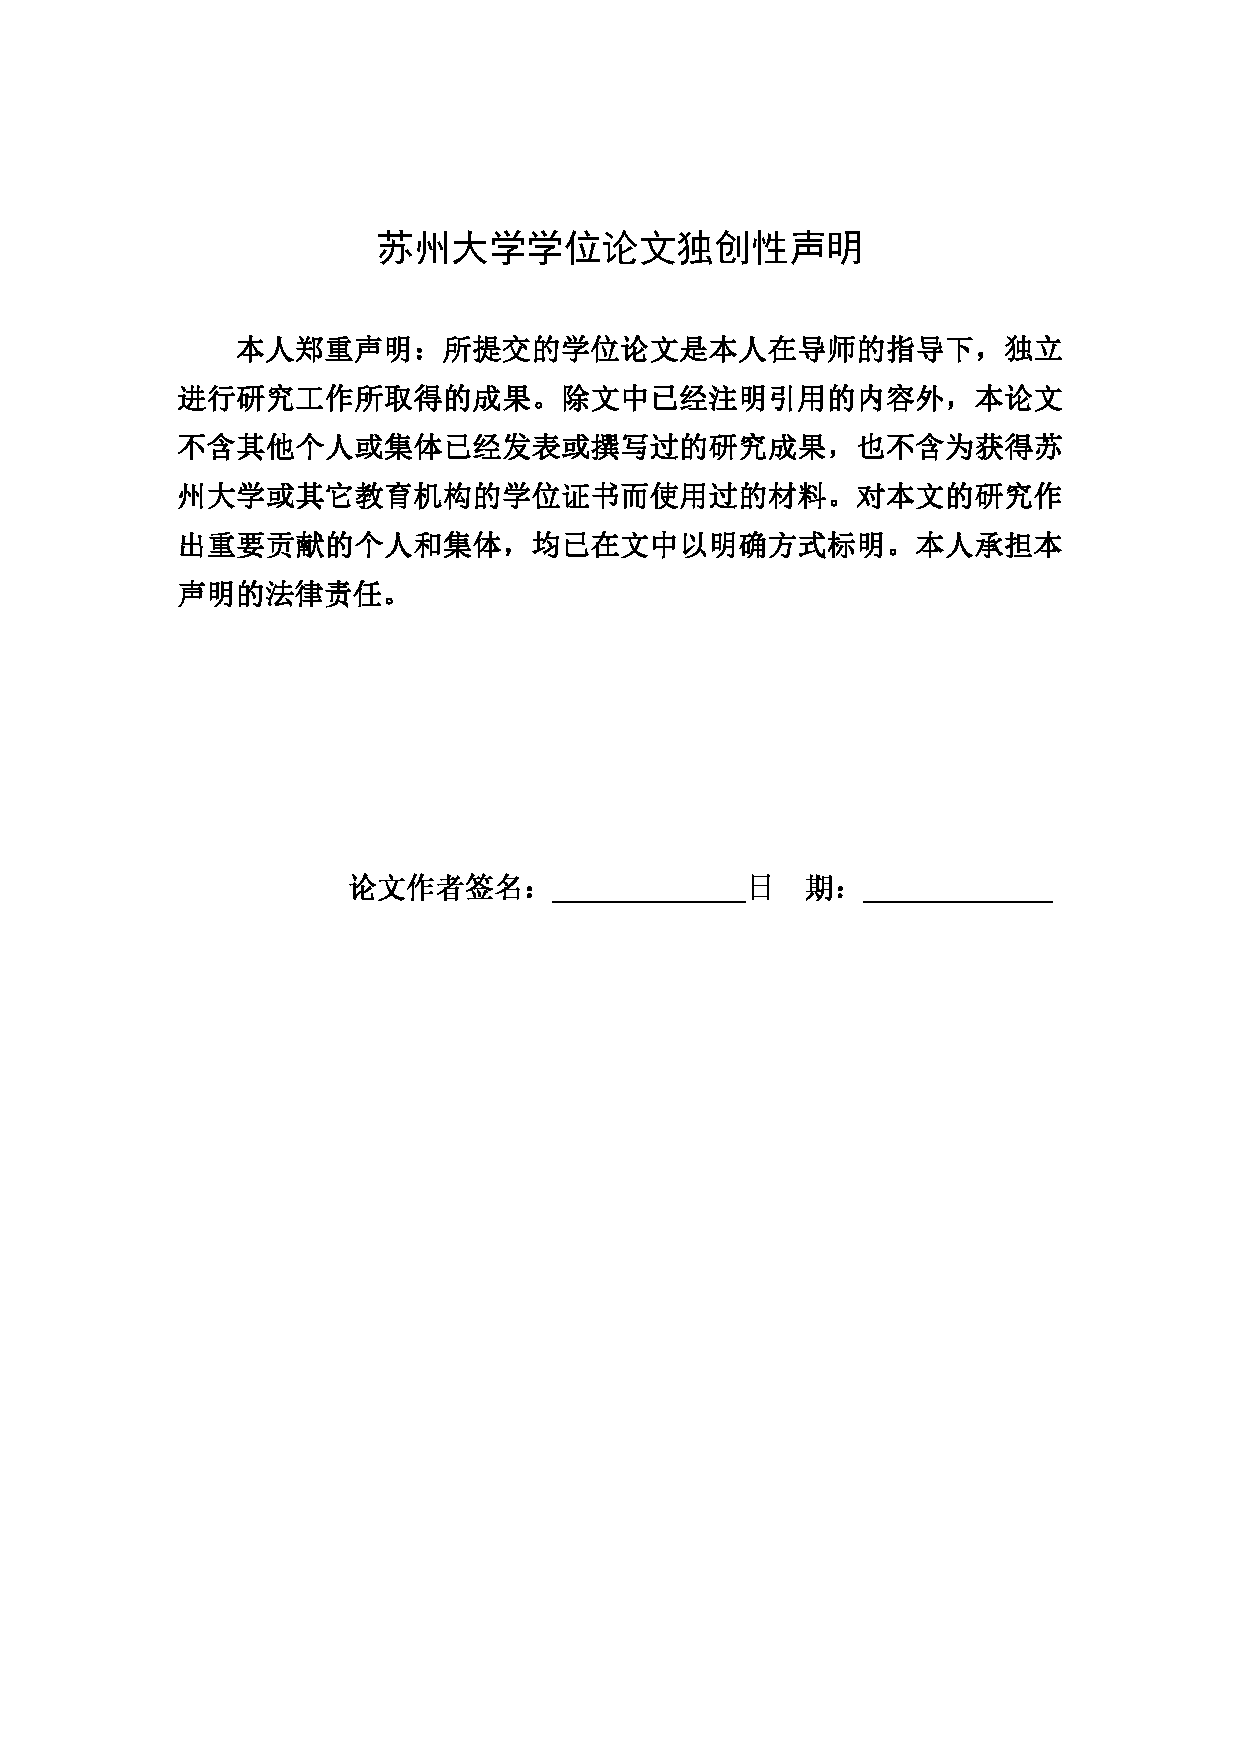
\includepdf[page=-]{pdf-pages/独创性声明.pdf}

\includepdf[page=-]{pdf-pages/空白页.pdf}
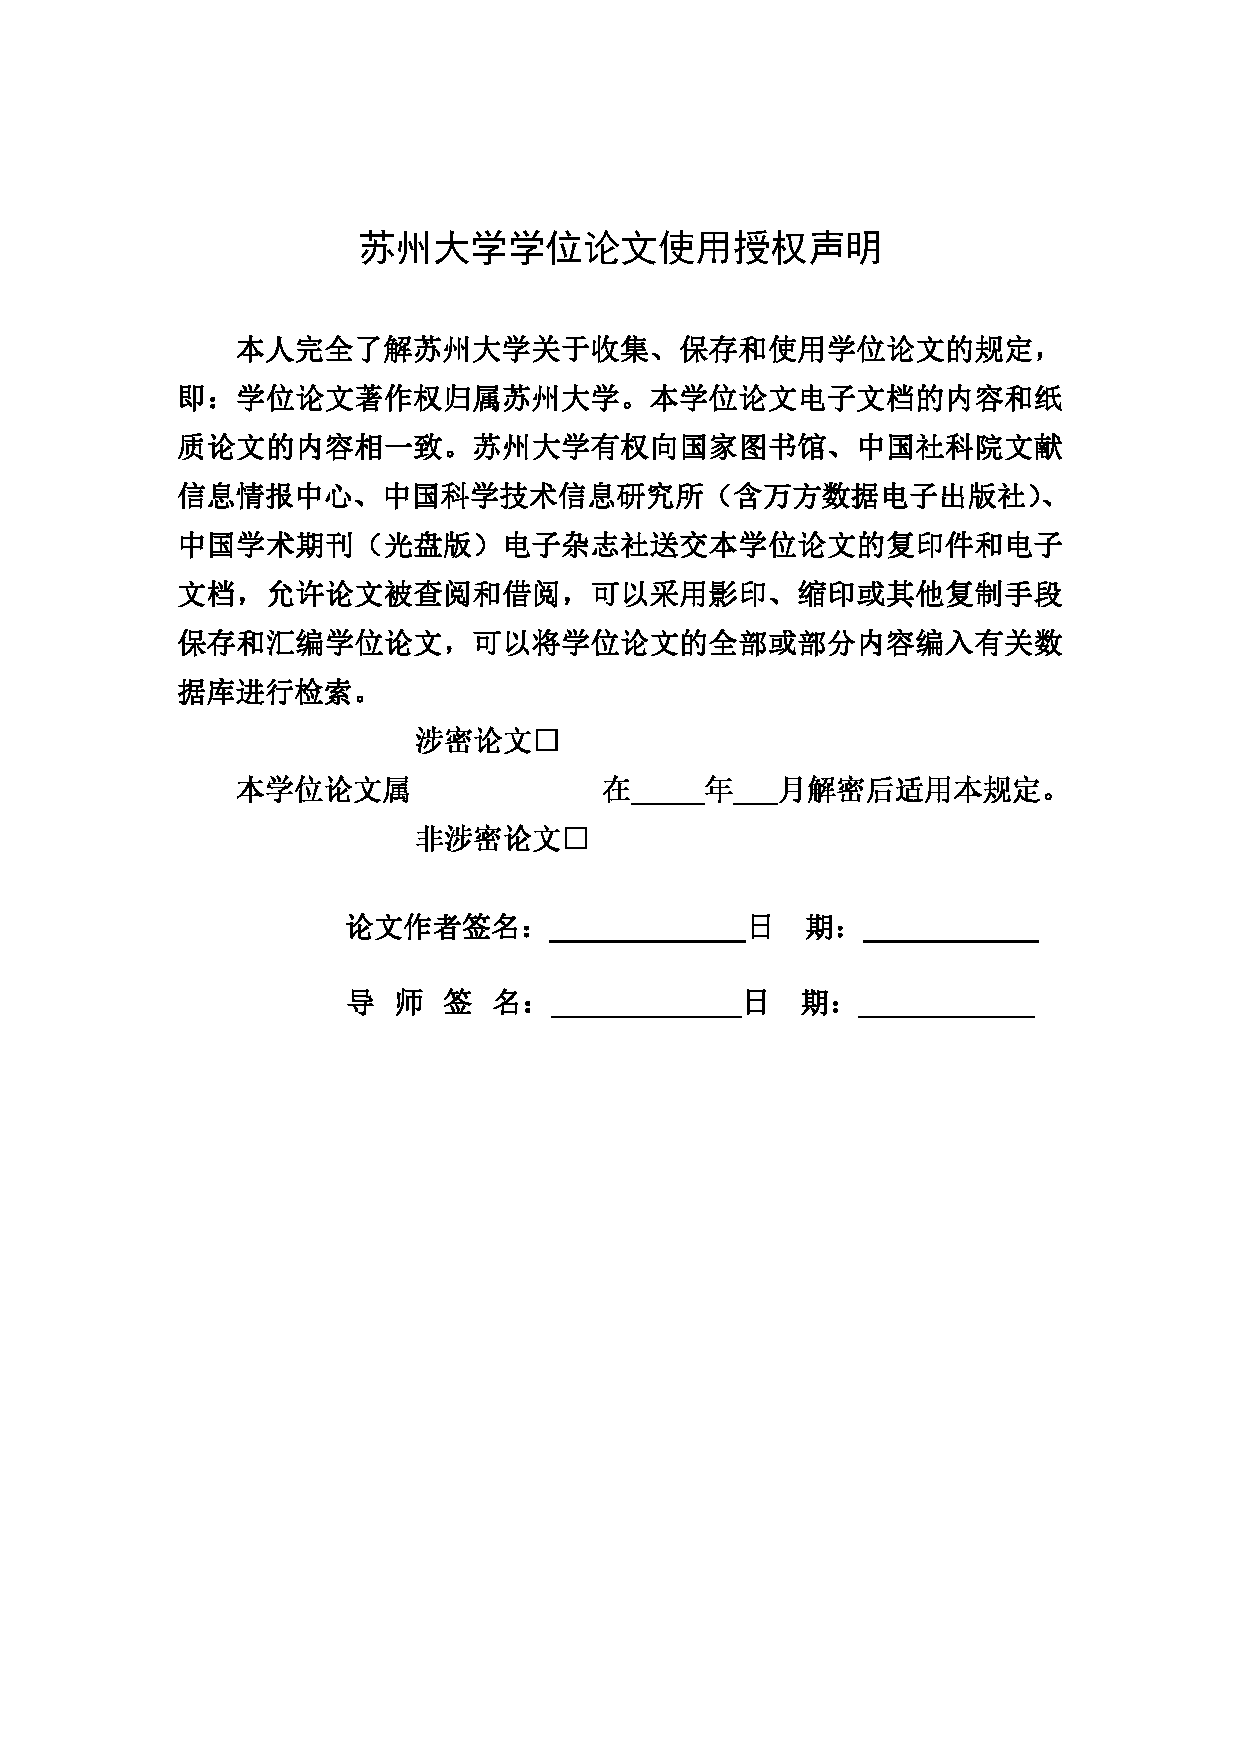
\includepdf[page=-]{pdf-pages/授权声明.pdf}

\includepdf[page=-]{pdf-pages/空白页.pdf}

% 正文前页码是大写罗马字母
\pagenumbering{Roman}
% 前言页眉页脚样式 % 摘要
\pagestyle{cnfrontmatter}
% !Mode:: "TeX:UTF-8"

% 中英文摘要
\begin{cabstract}

	问答匹配是自然语言理解中的一个重要的研究领域,有着广泛地实际落地应用,例如信息检索、智能问答以及对话系统等领域。
	问答匹配主要包含两个子任务:答案选择任务和问句复述识别任务。
	答案选择任务要求模型评估“问题-答案”之间的语义相关性,
	主要用于优化对于目标问题进行相关答案召回的质量;
	问句复述识别任务需要模型判定“问题-问题”之间的语义一致性,
	以此提高对于目标问题召回已知答案的同义问题的精度。
	现有的匹配方法基于预训练语言模型,将“文本对子”形成基于上下文的统一编码表示,进行分类。
	然而,单纯依靠预训练语言模型将面临1) 表征能力弱,难解困难样本;2) 问句意图感知能力差,两种局限性。


	本文基于上述问题展开以下三个方面的具体研究:
	1) 微调预训练模型的表征能力仍然难以解决答案选择任务中的困难样本。
	对抗样本在问答匹配任务上具有着良好的表现,但现有的方法粒度单一,产生的样本质量不高。
	因此,本文设计了双粒度的对抗训练方法,生成高质量的对抗样本,有效地提高模型的语义表征能力。
	% 1)预训练语言模型并未有效利用词块、短语和子句的独立语义信息表示,使其在匹配过程中容易错失精细粒度语义的感知。
	% 因此,本文提出一种多粒度交互推理网络,该方法对问题与答案进行多粒度语义编码,以丰富句子间的语义信息;
	2) 问句复述识别面临着“同质异构”以及“异质同构”样本难解的问题。传统的难样本生成方法存在时间效率低,生成质量差等问题。
	为此,我们设计了一种生成式的数据增强策略,显著提高了生成效率和质量。
	并且本文提供了“错题本”的训练方法,对于难解样本举一反三,简单有效地提高模型性能。
	% 预训练语言模型对特定任务的精细语义感知依赖于其微调数据的数量与质量。
	% 为此,本文提出一种定向数据增强策略,该方法利用诱导标签对生成网络进行引导,促进问题复述识别数据的自动扩展。
	% 与传统数据增强方法相比,本文方法生成样本的质量更高、语义表达更加多元化;
	3) 现有的预训练语言模型方法在解决问句复述识别问题时,没有有效利用问句的意图信息,例如时间,地点,做法等。
	导致模型忽视了意图信息,而容易被字面上的相近或差异所迷惑。
	为此,本文设计了基于变分自编码器的问句意图增强模型,有效地提升模型对于问句意图的感知能力。
	% 3)现有的研究缺乏对模型鲁棒性的深入探讨,尤其在数据资源相对稀缺的中文领域,模型的鲁棒性更加难以评定。
	% % 导致许多模型只能在特定的实验数据上呈现准确的结果,在实际应用中的表现却并不理想。
	% 为此,本文构建了一个符合中文语言学特征的评估数据集CQM$_{robust}$,
	% 其能够按照中文语言现象对问题复述识别模型进行系统化的鲁棒性测试,
	% 有助于分析现有预训练语言模型在该任务上的优势与不足。

	本文从对抗训练、生成式增强学习以及问句意图增强三个角度出发,一定程度上缓解了问答匹配领域中模型表征能力弱和问句意图感知能力差的问题。
	在公开数据集WPQA、TREC-QA、LCQMC、BQ和QQP上的实验证明了本文方法的有效性。
	\vskip 10bp
	\noindent
	{\heiti\zihao{-4} 关键词:}
	问答匹配,
	答案选择,
	问句复述识别,
	数据增强,
	意图识别
	
	\begin{flushright}
		{\heiti\zihao{-4} 作~~~~~~~~者:}金志凌

		{\heiti\zihao{-4} 指导老师:}洪~~~~宇
	\end{flushright}
	% \begin{flushright}
	% 	{\heiti\zihao{-4} 作~~~~~~~~者:}***

	% 	{\heiti\zihao{-4} 指导老师:}***
	% \end{flushright}
\end{cabstract}




\pagestyle{enfrontmatter}
% !Mode:: "TeX:UTF-8"

\begin{eabstract}

	Question Answer Matching is one of the most important research in Natural Language Processing.
	It mainly contains two subtasks, Answer Selection and Question Paraphrase Identification. 
	The objective of Answer Selection is to measure the semantic relevance between questions and answers, so as to optimize the recall quality of target answers in Question Answering (abbr., QA) scenarios. 
	Question Paraphrase Identification aims to determine the semantic equivalence between question pairs to improve the recall accuracy of the similar questions containing answer in QA scenarios. 
	Both of them are core technologies for the intelligent QA system and have been widely and practically utilized in search engines, community QA, intelligent customer service, etc. 
	Existing pre-trained language models are able to produce the unified encoding representation from text pairs, and the input structure and computation mode are suitable for handling Question Answer Matching. 
	However, the pre-trained language models still suffer from the limitations of insufficient fine-grained semantic perception and lack of robustness.

	Ground on the aforementioned problems, we conduct the specific research in the following three aspects: 
	1) The pre-trained language models fail to effectively leverage the independent semantic representation of word chunks, phrases, and clauses, 
	which tends to ignore the perception of fine-grained semantics in the matching. 
	Therefore, we propose a Multi-granularity Interaction Inference Network (abbr., MIIN),
	which encodes questions and answers with multi-granularity semantics to enrich the semantic information between sentences. 
	2) Although Fine-tuning the pre-trained language models are capable of improve its fine-grained semantic perception of specific tasks, 
	in fact this process greatly depends on the quantity and quality of fine-tuning data. 
	To this end, we propose a Directional Data Augmentation (abbr., DDA) strategy. 
	DDA utilizes the directional label to guide the generation network for automatic expansion of Question Paraphrase Identification dataset. 
	Compared with the traditional data augmentation methods, the samples generated by DDA are of higher quality and more semantic diversity. 
	3) Existing research lacks the in-depth exploration on the robustness.
	Especially in the Chinese domain, where data resources are relatively scarce, 
	the robustness of the models is more challenging to be evaluated. 
	Therefore, we construct a Question Paraphrase Identification dataset called CQM$_{robust}$, which is in line with the characteristics of Chinese linguistics. 
	CQM$_{robust}$ systematically evaluates the robustness of the models according to linguistic phenomena, 
	and assist us analyze the advantages and disadvantages of the existing pre-trained language models in Question Paraphrase Identification.
	
	We alleviate the problems of insufficient fine-grained semantic perception and robustness in Question Answer Matching from three perspectives: multi-granularity interaction, directional data augmentation, and robustness evaluation. 
	Our experiments on public datasets WPQA, LCQMC, and CQM$_{robust}$ all verify the effectiveness of the proposed methods.
	\vskip 10bp
	\noindent
	{\bf\zihao{-4} Key words: }
	Question Answer Matching,
	Answer Selection,
	Question Paraphrase Identification,
	Data Augmentation,
	Robustness

	\begin{flushright}
		{\bf\zihao{-4} Written by} Hongyu Zhu
		
		{\bf\zihao{-4} Supervised by} Min Zhang and Yu Hong
	\end{flushright}
	% \begin{flushright}
	% 	{\bf\zihao{-4} Written by} ***
		
	% 	{\bf\zihao{-4} Supervised by} ***
	% \end{flushright}
\end{eabstract}



\includepdf[page=-]{pdf-pages/空白页.pdf}

% 目录不设置页眉和页码
\makeatletter
\let \asas \ps@plain
\let \ps@plain \ps@empty
\makeatother
\pagestyle{empty}

% 生成目录
\tableofcontents
\setcounter{secnumdepth}{4}

\makeatletter
\let \ps@plain \asas
\let\asas\relax
\makeatother
\cleardoublepage  %目录3页以上,使用cleardoublepage

% 正文页码样式
\mainmatter
% 正文页眉页脚样式
\pagestyle{mainmatter}
% 正文页码是阿拉伯数字
\pagenumbering{arabic}

% % 正文

\chapter{绪论}

本章将对问答匹配任务展开详细介绍。
首先,本章阐述了问答匹配任务的研究背景及意义。
% 其次,本章介绍了该任务的国内外研究现状。
接着,本章总结了前人的科研工作,分别从基于表示、交互和数据增强三个方面,详细介绍了国内外研究现状。
然后,本章分析并总结了问答匹配领域现有的科学问题及研究难点,并针对以上问题和难点,阐述了本文的主要研究内容。
最后,本章简述了全文的组织架构。

\section{研究背景}

%% 问答系统的重要性
% 现有互联网信息获取的主要渠道为搜索引擎,其根据用户的提问返回一系列相关的网页链接。
% 人们通常在互联网上获取信息的主要渠道为搜索引擎,其根据用户的提问返回一系列相关的网页链接。
% 近年来,互联网技术高速发展,网络数据也呈爆炸式增长,
% 这导致用户需要花费大量的时间与精力从繁杂冗余的搜索结果中获取有用信息。
% 同时,网络上数据的质量参差不齐,传统搜索引擎无法有效甄别数据的合理性。
% 在此背景下,智能问答系统应运而生。

%% 问答系统的细分及匹配技术的重要性
问答匹配(Question Answer Matching)是自然语言处理(Natural Language Processing,简称NLP)领域重要的研究方向。
目前已在多种场景,如问答系统、客服机器人、语音助手等,得到广泛应用,当前主流的搜索引擎(百度、谷歌等)也已引入基于深度学习的问答匹配技术,以提供更加精准可靠的搜索结果。
问答匹配任务可以通俗地理解为面向问答场景文本的语义匹配任务。
作为问答匹配的子任务,答案选择(Answer Selection)以及问题复述识别(Question Paraphrase Identification)从语义匹配的不同角度为实际应用提供服务。
答案选择任务需要模型根据给定问题与候选答案的相似性,对候选答案进行排序,选择出相关性较高的答案进行返回。
问题复述识别任务则需要模型识别问句对子之间的语义一致性,即两个问句的意思是否一致,从而从已知答案的庞大问答对子中找出与用户提问最相关的问题,并返回其答案。
从答案选择以及问题复述识别任务的定义可知,两者分别从“问题与答案”的语义相关性以及“问题与问题”的语义一致性的两个角度,为智能问答系统,搜索引擎等实际应用提供支持。
其对知识获取、信息检索等领域也具有重要影响力。因此,问答匹配技术的研究具有十分重要的意义。

% 问答匹配的发展(预训练) 及缺点
随着预训练语言模型的发展,其优秀的特征提取和语义编码能力在NLP领域带来了显著的提升,其中也包括问答匹配任务。
问答匹配技术的研究一直备受关注,基于预训练语言模型的深度学习方法也成为了问答匹配任务的主流方法。
但是尽管研究的方法不断改进,却始终存在着两个挑战性的问题:其语义表征能力难解困难样例和问句意图感知能力弱。
首先,困难样本难解的根本原因是模型的语义表征不准确,没有精细地感知到语句中细微且关键的要素。
利用困难样本生成技术,例如对抗攻击方法,构造具有迷惑性的样本,加入模型的训练,是提高语义感知和表征能力的有效方法。
研究如何高效且高质量地生成困难样本对于提高问答匹配模型性能具有着重要的意义。
其次,问句意图感知能力弱也是当前问答匹配技术需要解决的另一个关键问题。
对于问句来说,意图信息是十分关键的。
例如:“您今晚什么时候吃饭?”和“您今晚什么地方吃饭?”,尽管字面十分相似,但是前者的意图是对时间提问,而后者是对地点提问。
仅仅凭借预训练语言模型的方法容易被相近的字面所迷惑,而忽视了更加关键的意图信息。
这些问题目前还缺少有效的解决方法。


% 但是,这并不意味着模型在实际应用中仍能保持其高性能。
% 在真实的语言场景下,一些简单且易于回答的问题,最前沿的模型却会给出错误回答。
% 在实际应用中,问答匹配技术仍处于起步阶段,需要不断革新,使问答系统更加高效、准确。

\section{研究意义}
问答匹配包括答案选择以及问句复述识别两个子任务。问答匹配无论是对实际业务应用或是自然语言处理的科学研究都有着重要的研究意义。
此处从以下三个方面阐述其研究意义:

\textbf{\songti(1)广泛的实际业务应用}
问答匹配任务有着广泛的实际业务需求应用,例如搜索引擎、自动问答、智能客服等领域。
其需要系统能够充分理解用户所输入问句的语义,并从已有的数据源中匹配出相关性最佳的结果。
现有的主流搜索引擎中已经引入基于深度学习的问答匹配技术。
用户输入问题后,搜索引擎内部利用问答匹配和机器阅读理解等技术,解析出精确的答案作为第一条结果返回,极大提高用户搜索体验。
此外,例如信息检索技术可以归结为是用户输入的查询与文档资源的语义匹配,自动问答系统则是通过用户查询与已有候选答案或者是已有“问答对子”的问句进行匹配。
包括众多商家如淘宝、京东等都接入了智能客服系统,用户解决海量的客户问题及反馈。
利用这种方式可以高效的解决用户的常见问题,降低运营成本,提升用户体验,这也是问答匹配技术的一项成熟的应用。
问答匹配是自然语言理解中的核心问题,其泛用性成为许多前沿智能系统的基础技术。


\textbf{\songti(2)对问答系统的重要意义}
传统的搜索引擎根据用户查询返回相关的网页,这样的方式导致用户无法快速便捷地获取关键信息。
而由深度学习技术兴起的自动问答系统以“一问一答”的智能形式,给予用户良好的交互体验。
通过这种方式可以精确定位用户意图,从而快速高质量地满足用户的信息需求,达到降低成本,提高用户体验的效果。
答案选择技术提供了“问题-答案”相关性语义的支持,根据用户所输入的问句的语义信息,从已有的候选答案数据中匹配出最佳结果。
例如,该技术应用于基于知识库的问答系统(Knowledge Base Question Answering, 简称KBQA),为用户输入的问题召回相关性最高的知识,以用于模型结合问句以及知识之后产出答案。
问题复述识别则从“问题-问题”之间的语义一致性出发。根据用户输入的目标问句,从已知答案的候选“问句-答案”对子中,匹配出语义相同或高度相似的复述问句,将其答案返回给用户。
例如对于常用的检索式问答系统,以及主流的搜索引擎(如百度,谷歌等)而言,问句复述识别是实现该类系统的关键。
因此,提高问答匹配技术对于自动问答,信息检索等智能系统的准确性和可靠性的具有非常重要的意义。


\textbf{\songti(3)为自然语言处理研究提供支持}

问答匹配任务可以通俗地理解为面向问答场景文本的语义匹配任务,其任务的核心在于理解句子对的语义,并且根据任务场景作出相应的判断。
其语义理解和匹配的能力为自然语言处理领域的其他任务提供了强大的支持。
例如,在常识问答(Commonsense QA)任务中,需要模型在获取到问题之后,检索与问题相关的常识知识。借由这些知识的语义交互,模型才能产出该问题的答案。
问答匹配技术能够根据问题,有效地检索出知识库中与之相关的常识信息,返回给模型。问答匹配技术的召回的知识是否准确和可靠,也成为了常识问答模型是否能够准确回答问题的关键。
在开放域阅读理解(Open-domain Machine Reading Comprehension)任务中,首先需要借助问答匹配技术,在庞大的文档资源中,匹配出较为相关的段落,继而在匹配结果中利用阅读理解技术截取答案。
这种二段式的阅读理解方案在当今数据文本爆炸式增长的时代,不用处理过长的文本,可以大幅减少计算成本,并且结果也比传统的长文本处理方式更加精确,目前已经被广泛地应用。
此外,问答匹配任务对于文本语义的挖掘需求非常精确,这样的语义理解能力在传统的自然语言处理任务例如文本蕴含、篇章关系分析等方向都有着重要意义。

综上所述,问答匹配是自然语言处理领域的一项核心的研究任务,提高问答匹配的性能能够从根本上提高智能问答系统,搜索引擎等应用的准确性和可靠性,并且问答匹配对于其他自然语言处理任务的研究和发展都有着重要意义。

\section{国内外研究现状}

问答匹配是文本匹配领域面向问答场景文本的分支,早期文本匹配方法主要为向量空间模型(Vector Space Model,简称 VSM)\cite{salton1975vector}和基于概率检索模型的BM25\cite{robertson1994some},由Salton等人和Stephen等人提出。
主要用于建模词汇层面的字面匹配问题,该类方法缺乏对文本语义的深度理解,无法有效利用文本中的上下文语义。
随着深度学习方法的兴起,基于神经网络构建的文本匹配模型能够建模句子整体语义的高维特征表示。
这类方法突破了传统匹配方法停留在字面匹配的局限性,将文本匹配方法引入了新的研究方向。
深度文本匹配模型按照模型处理结构和语义信息表征的不同可以分为两大类,包括基于表征学习的方式和基于交互的方式。
而数据增强(Data Augmentation)作为一种资源扩展和难样本增广的方法,广泛地用于提高深度文本匹配模型的语义表征能力和难样本解决能力。
此处从以下三个方面详细分析该任务的国内外研究现状:

\textbf{\songti (1)基于表征学习}

基于表征学习的方式集中于研究如何构建语义表示层,用于将文本表示为高维向量。
这类方法通常使用孪生网络结构(Siamese Network)构建神经网络,这是一种共享参数的双通道结构。
利用双通道分别对“句子对”的两个句子进行独立编码,将其语义信息转化为高维特征向量。
得到两个分别表征两个句子的语义信息后,继而使用相似度计算方法,例如余弦相似度、欧几里得距离等,计算文本间的语义关系。
He等人首先提出的基于深度网络的语义模型DSSM\cite{huang2013learning},最先利用孪生结构的全连接神经网络对文本提取语义特征。
并且在DSSM基础上将全连接神经网络改进卷积神经网络(Convolutional Neural Networks,简称CNN)作为特征提取器的CLSM\cite{shen2014latent},以及长短期记忆网络增强(Long Short-Term Memory,简称LSTM)的LSTM-DSSM\cite{palangi2014semantic}模型。
He等人提出了一种孪生CNN的表示学习结构\cite{he2015multi},他们的实验比较了余弦相似度、欧氏距离和元素级作差等方法在相似度关系计算上的效果。

基于表征学习的方式也有着难以判断语义焦点、无法利用关键上下文的语义信息等缺点。
为了能够有效地缓解上述的问题,文本中的关键上下文需要能够加强其表示权重。
例如,Santos等人提出的AP-BiLSTM\cite{santos2016attentive}是将注意力机制与LSTM相结合的表示学习模型,其验证了注意力机制聚焦语义的正面作用。
Wang等人\cite{wang2016sentence}将两个句子按照词级分解为相似和不同两个集合,并通过CNN提取相似特征和可区分特征。 
Lai等人则是关注到由于中文分词可能引起的歧义,提出了一种基于词格(word-lattice)的CNN模型(LCNs)\cite{lai2019lattice}。

随着预训练语言模型(例如BERT\cite{devlin2018bert})的成熟应用,其强大的语义编码能力为文本匹配任务带来了显著的提升。
前人应用预训练语言模型作为双通道的编码器,对句子对分别进行独立地编码。
例如,Lyu等人\cite{lyu2021let}同样关注到,尽管应用了预训练语言模型,但是中文匹配任务上出现的分词歧义问题仍然难以解决.
于是提出了外部知识网络HowNet\cite{dong2003hownet}和词格构建图结构,利用图神经网络进行编码。
Wang等人提出了DABERT\cite{wang-etal-2022-dabert}的双流注意力方法,利用亲和注意力和差异注意力分别构造了句子对的相似特征和差异特征进行融合,得到更加完善的句子表示。


\textbf{\songti (2)基于文本交互}
 
基于交互方式的研究认为,不管是“问题-答案”或是“问题-问题”,句子对之间都存在着某种联系,双通道的独立编码方式(基于特征学习的方式)没有很好地利用这一联系。
基于交互的方式认为建模语义编码的过程应当更早地进行两段文本的交互,以此挖掘文本之间的交互特征,这样的特征能够很好地找到文本对子之间的语言联系。
前人的实验证明,基于文本交互的模型方法能够更好地在文本之间双向地捕捉焦点信息,且在特征表示中凸显句子对中交互性较强的语义信息,这些语义信息往往起着关键性因素。
例如,Pang等人提出的MatchPyramid\cite{pang2016text}受到图像处理的启发,用文本对子之间的交互构建了相似度矩阵,并利用CNN网络作为特征提取器对相似度矩阵进行编码。
Gong等提出深层交互推理模型DIIN\cite{gong2017natural},其构造元素级高阶交互,并使用密集连接卷积网络提取特征。DIIN在深层交互的同时,一定程度上保留了原始特征信息。

同样,随着注意力机制的广泛应用,其作为一种理想的交互计算方法,也被广泛应用在交互式方法的研究中,并且有着良好的表现。
例如,Wang等人提出了“匹配-聚合”框架下的 BiMPM 模型\cite{wang2017bilateral},该模型进行双边多角度的匹配操作以获得交互信息。 
Chen等人提出的ESIM\citet{chen-etal-2017-enhanced}模型则在LSTM的基础之上进行交互式推理,其通过元素点积和减法来锐化交互信息。
受ResNet\cite{he2016deep}的启发,Kim等人提出了一种结合了循环神经网络RNN、残差链接以及注意力机制的方法DRCN\cite{kim2019semantic}。
上述的方法都在语义表征过程中,利用注意力机制在句子对之间进行语义交互,凸显了句间的特征联系,并将其更好地融入句子的语义表示。

预训练语言模型也因其优秀的特征提取能力和多层的注意力机制带来的优秀交互能力,在问答匹配的交互方法上取得显著成果。
预训练语言模型在文本匹配任务上的交互方式是,通过将句子对拼接,作为统一的输入进入模型,由注意力机制等方式进行信息交互。
例如,Zhang等人提出了一种基于 BERT 的关系学习网络 ($R^2$-Net)\cite{zhang2021making},其利用多粒度语言单元的交互关系,更深层地学习标签所带来的语义信息。
以及,Xu等人最新提出的ISG-BERT\cite{xu2022semantic}将两个句子的句法对齐结果和语义匹配信号集成到关联图中,以获得更细粒度的匹配过程。

\textbf{\songti (3)数据增强方法}

前人的研究表明,数据量小、样本难度低等问题容易引起模型的过拟合问题。
数据增强方法通过扩大训练数据、提高数据难度和质量等方式,达到优化模型性能的效果。
回译(Back Translation,简称BT)是一种最常见的数据增强方式,Yu等人\cite{yu2018qanet}利用英法回译,先将数据转换成法语,再回译成英语,利用翻译过程中的差异达到用不同表述复述原句的效果。
但是,回译策略受到专业名词、地方文化不同、语言之间的语用习惯差异大等问题的影响,许多内容难以准确的翻译,这也会导致回译数据产生语义偏移和阅读起来不自然等问题。
Wei等人提出了一种简单数据增强策略EDA\cite{wei2019eda}在原样本的文本上随机删除、插入、交换字符,以及进行同义词替换四种操作构造新的增强样本。
尽管EDA策略实现简单,效率极高,但是这样的随机操作容易产生有着严重语法错误、语义偏移、甚至完全不可读等情况。
将这样的样本加入训练数据,会导致模型训练过程有着极大的噪声,会导致其数据增强效果的下降。

为了缓解上述的问题,Jin等人提出的TEXTFOOLER\cite{jin2020bert}方法利用外部知识库WordNet提供同义词列表进行替换,再使用通用句子编码模型(Universal Sentence Encoder,简称USE)\cite{cer2018universal}监测替换后的句子和原句是否有较大的语义偏移,若有,则舍弃该样本。
同样基于WordNet的同义词替换策略,PWWS方法\cite{ren-etal-2019-generating}则提出了一种概率加权的词显着性方法来确定词替换顺序。
而Li等人提出的BERT-ATTACK\cite{li2020bert}方法,为了能够缓解同义词替换带来的不自然和语法错误的问题,利用语言模型的掩码预测任务(Masked Language Model,简称MLM)代替同义词替换,即将需要替换的词遮蔽,使用MLM任务生成该位置的候选词。

前人的研究,例如Morris等人\cite{morris-etal-2020-reevaluating}发现,基于同义词替换或是随机字符修改的方法容易引起语法错误,语义偏移,阅读不自然等问题。
前人也提出了其他方式的数据增强方法来改善这一问题。
例如,Gary等人\cite{garg2020tanda}提出的TANDA(Transfer and Adapt Pre-train Model,简称TANDA)利用了多段迁移学习的方式,在通用领域或是相似领域的数据上预先学习一部分知识,作为样本数据的扩充。
为了提高生成的效率和质量,前人开始尝试生成式的数据增强方法。
随着自回归(Auto-Regeressive)的生成式模型不断成熟,越来越多的工作开始以端到端(sequence to sequence,简称seq2seq)模型作为数据增强方法。
例如,Hou等人\cite{hou-etal-2018-sequence}提出了一种基于seq2seq模型的填槽式样本生成方法,而Kumar等人\cite{kumar-etal-2020-data}对自编码器的BERT以及自回归的GPT-2\cite{radford2019language}和BART\cite{lewis2019bart}等模型进行文本增强的对比。
基于seq2seq的生成式模型目前已经具备了生成符合人类语言习惯的优质文本的能力,在生成效果的多样性和流畅性上要优于同义词替换等方法,同时也具备良好的时间效率。


% 但是,生成式的方法受限于数据问题,并非一个普适的方法。该类方法需要至少满足两个条件中的一条,即数据本身具备可生成的条件或是调用外部同领域的其他可生成的数据集获取知识。
% 如何有效地利用生成式模型进行数据增强也成为了一个值得关注的研究方向。


\section{关键问题和研究难点}

由上述研究现状可知,基于深度学习技术的的问答匹配方法已经趋于成熟,取代了传统的匹配方案。
然而,由众多的研究工作表明,问答匹配技术仍然在各个方面有着不完善的缺点,在实际应用中仍面临着诸多挑战。
本节主要总结问答匹配任务的现有的关键问题及其原因,以及面向该问题的研究难点。

\subsection{关键问题}

% % 语言理解能力
% % 鲁棒能力(迷惑样本)
% 传统的基于字面匹配的匹配方案(如BM25)主要根据“文本对子”中的字面关键词进行匹配,无法关注文本的深层语义。
% 其方法通过对文本中关键词的词频和文档长度等因素进行加权计算,这导致了传统的匹配方法经常出现误差,无法准确识别文本之间的语义关系。
% 如,{\kai{“您今天晚上准备什么时候吃饭?”}}和{\kai“您今天晚上准备什么地方吃饭?”},这两句话具有字面有着高度的重复的关键词,传统的匹配方法往往难以找到关键点,而将其判断为同样语义的问句。

深度学习技术突破了传统匹配方法(如BM25等)只能通过字面关键词进行匹配的限制,能够将文本这样离散化的数据作为输入,通过神经网络编码得到语义信息的高维特征表示向量,再利用文本对子在向量空间的位置和距离等信息判断语义关系。
而近年的预训练语言模型,作为自然语言处理领域的一项突破,其出色的特征提取和上下文感知能力为问答匹配任务带来了显著的提升。

然而,受到微调的数据规模、难度、质量等方面的限制,仅仅依靠预训练语言模型对文本的语义理解程度远远不够,仍存在一些问题。
1)现有的答案选择方法,在非事实性问题的场景下,由于其答案通常呈现为较长的段落级回答,导致其难以准确提取语义核心,而性能表现较差。
于此同时,该类模型受到轻微的扰动(例如同义词替换),即会更改预测的答案,鲁棒性差。
2)在问句复述识别任务中,“同质异构”与“异构同质”类样本是模型最难以判断的两类困难样本。
这两类样本需要模型具有感知其精细语义的能力,当前的问句复述识别方法在这两类样本上的表现仍然欠佳。
3)现有的问句复述识别方法,忽视了问句意图的重要作用,导致其对于意图感知能力差。
而意图是否一致对于语义一致性的判断是十分重要的,如何增强模型对于意图的感知也是问句复述识别的一项关键问题。
因此,综上所述,强化模型对于关键语义的提取能力,以及提高模型对于问句意图的感知能力应该作为问答匹配任务的重点研究内容。


\subsection{研究难点}

基于现有问答匹配方法所存在的关键问题,我们将研究难点总结为以下三点:

\textbf{\songti (1)模型的语义提取能力弱,鲁棒性差}

预训练语言模型可以接收“文本对子”的输入,利用注意力机制,形成上下文相关的统一语义编码表示。
然而,在面向非事实性问题的答案选择任务中,候选答案呈现为较长的段落级回答,这使得全局注意力的噪声较大,无法准确提取段落的核心语义。
模型在训练过程中,面临着语义提取能力弱,并且容易受到噪声干扰等问题。
在不影响句子语义情况下的轻微扰动都常常引起模型预测结果的改变,例如,关键词的同义词替换,句子向量的细微扰动等。
这种不稳定性正是因为其关键语义的感知偏差导致的,模型在较长文本的场景下,无法抓住文本的核心语义信息,进而导致了抵抗不了轻微干扰的弱鲁棒性。
如何设计一种在非事实性答案选择任务场景下,设计一种增强模型关键语义提取能力和稳定性的训练方法,是一项重要的研究内容。


\textbf{\songti (2)“同质异构”和“异质同构”类样本难解}

在问句复述识别任务中,细微的语义差异会导致文本之间的语义关系发生很大的变化。
“同质异构”样本指两个文本具有相同的语义但是字面的表现形式差异较大,其实际关系应为“复述”,而模型由于其字面差异过大判断为“非复述”。
而“异构同质”样本指两个文本具有相近的字面表示形式,但其语义不同,其实际关系应为“非复述”,而模型由于其相似的字面关系判断为“复述”。
预训练语言模型由于其预训练任务与下游任务之间的差异,导致其对于精细的语义的感知并不敏感。
如例 1-1 所示的“异质同构”类样本,两个问句只有一字之差,编辑距离仅为1,但是却代表着不同的语义。
模型能够判断这类样本的前提是需要能够感知到这样关键的细微差别。
\begin{quotation}
    \noindent \textbf{\songti 例1-1}(“异质同构”问题对子样例)
    
    \noindent \textbf{问句1:} 淘宝邮政编码怎么\underline{填}?
    
    \noindent \textbf{问句2:} 淘宝邮政编码怎么\underline{改}?
    
    \noindent \textbf{编辑距离:} \underline{1} \qquad \textbf{关系:} \underline{非复述}
    
\end{quotation}

如例 1-2 所示的“同质异构”类样本,两个文本之间的表述差异较大(编辑距离为8),但是两者却有着相同的语义,这对于模型而言也是巨大的挑战。

\begin{quotation}
    \noindent \textbf{\songti 例1-2}(“同质异构”问题对子样例)
    
    \noindent \textbf{问句1:} 管理者怎样才能让员工服从?
    
    \noindent \textbf{问句2:} 怎样使员工服从领导?
    
    \noindent \textbf{编辑距离:}  \underline{8}  \qquad \textbf{关系:} \underline{复述}
    
\end{quotation}

然而,现有的问句识别数据集中,该类别的难样本在训练数据中占比极少,模型无法在训练过程中获得感知其精细语义的能力。
数据增强方法是缓解该问题的重要方法,但是现有的数据增强难以产出高质量的“同质异构”和“异质同构”样本,成为问句复述识别任务的研究难点之一。

\textbf{\songti (3)问句意图感知能力弱}

问句意图作为识别问句语义一致性的重要信息,但是现有的问句复述识别方法忽略了这一问题。
如例 1-3 所示,问句1的问句意图是询问人,即为“Who”类型的问题,而问句2的问句意图是“What”类型,即在询问定义。
\begin{quotation}
    \noindent \textbf{\songti 例1-3}(不同问句意图的非复述问题对子样例)
    
    \noindent \textbf{问句1:} \underline{Who} exactly is successful?

    \noindent $<$\textit{译文:到底谁可以称为一个成功人士?}$>$
    
    \noindent \textbf{问句2:}  \underline{What} exactly is success?

    \noindent $<$\textit{译文:到底什么可以称为成功?}$>$
    
    \noindent \textbf{关系:} \underline{非复述}
    
\end{quotation}

两者的虽然字面相近,但是问句意图却是完全不同的,这一点从翻译成英文后的疑问词可以明显的发现。
提高模型对于问句意图的感知能力,能够使其对于问句对子之间的语义关系判断更加精确。
现有的模型方法很少从问句意图的角度出发,因此,如何提高模型对于问句意图的感知能力是当前研究的一个难点。


\section{研究内容与组织结构}

针对上述问答匹配任务的关键问题及研究难点,本文从提高模型对长文本和精细文本的语义提取能力,以及增强模型问句意图感知能力等多个角度出发,提出了三个研究工作。
本节对其研究内容,以及论文的整体组织结构安排进行概述。

\subsection{研究内容}

本文主要针对问答匹配模型的关键语义提取能力及问句意图感知能力进行研究,对现有的前沿匹配方法进行优化。
本文研究内容具体可分为以下三个模块:

% \textbf{\songti (1)基于多粒度交互推理的答案选择方法研究}
\textbf{\songti (1)面向非事实性答案选择任务的双粒度对抗训练方法研究}

本文前期研究显示现有的答案选择方法在非事实性场景下,关键语义提取能力弱,受到轻微噪声影响即会改变预测结果。
对抗训练方法作为数据增强方法的一种,具有生成困难样本进行数据增强,提高模型稳定性的能力。
但是前沿的对抗训练方法往往集中于对于样本进行单一粒度的扰动(字符级,词级,句子级)。%%%%%%%%%%%%%%%%%%%%%%
这种方式生成的对抗样本质量低,模式单一,容易被模型捕获。
% 其在BERT编码信息之上再次执行多粒度卷积编码,并且将多粒度交互信息与原始分类特征融合,形成蕴含关键线索的精细语义表示。
% 其二,候选答案中不同句子与问题的关联性具有显著差异,但现有模型的训练过程,并未考虑子句的权重差异。
% 为此,本文提出了一种句子级的损失优化策略,侧重提升关键语句在答案选择过程中的作用。

\textbf{\songti (2)面向问题复述识别的定向数据增强方法}

现有的问题复述识别模型对特定任务中精细的语义表示需求并不敏感。
预训练语言模型的微调阶段能有效提高模型对任务相关的细微语义感知力,但其极大依赖于训练数据的多样性与可靠性。
数据增强策略能够有效扩充蕴含精细语义关系的数据样本,在一定程度上能够提高模型的任务适应性。
传统的简单数据增强策略以及回译策略能够高效地扩充数据数量,但是其仅能构造与原样本语义相同的数据,并且无法保证构造样本的语法正确性和标签一致性(即样本不合格),这些包含错误知识的数据对模型产生负面影响。
本文提出一种基于生成模型的定向数据增强策略(Directional Data Augmentation,简称DDA),在生成模型的输入中添加定向标签,引导其生成期望的复述句或非复述句。
此外,本文设计了一种多模型集成的标签投票机制,并用其修正增强样本的潜在标签错误,以此提高扩展数据的可靠性。

\textbf{\songti (3)面向问题复述识别的模型综合能力鲁棒性研究}

鲁棒性是反应模型能力的一项重要评价指标,缺乏鲁棒性的模型在现实应用中的性能往往并不理想。
目前一些研究已经开始关注模型鲁棒性的研究,但大多只针对某种特定场景下的数据,或是只使用了少量的数据变化方法,缺乏综合性的评估方案。
为了系统地评估问题复述识别模型的综合能力,本文构造了CQM$_{robust}$中文评估数据集,其包含3大类语言特征、13个测试子类,共计32种蕴含不同语言学特征的数据测试项。
同时,CQM$_{robust}$数据集中的所有问题均源于百度搜索日志中的真实问题,与实际应用场景匹配。
实验结果证明,CQM$_{robust}$比传统数据集难度更大,更具有挑战性,且能够对按照语言学现象对模型的能力进行详细评估,这有助于诊断不同模型的优点和缺点,为模型的优化方案提供参考。


\subsection{论文组织结构}

本文共分为六个章节,论文的组织结构以及各个章节的主要内容如下:

第一章 \quad 绪论。本章首先介绍问答匹配任务的研究背景和意义,然后分析了该任务的国内外的研究现状,总结了当前的关键问题和研究难点。最后,介绍了本文的研究内容和论文组织结构。

第二章 \quad 任务定义及评价方法。本章介绍了问答匹配的任务定义、实验数据语料以及主流的评价指标。

第三章 \quad 基于多粒度交互推理的答案选择方法研究。本章首先介绍了该方法的动机,然后重点阐述了该方法的模型架构和具体实现细节。最后,本章通过实验验证所提方法的有效性。

第四章 \quad 面向问题复述识别的定向数据增强方法。本章首先介绍该策略的动机,然后介绍了定向数据增强策略据的实现细节,最后给出实验结果及分析。

第五章 \quad 面向问题复述识别的模型综合能力鲁棒性研究。本章首先分析了鲁棒性对于问题复述识别模型的必要性,其次介绍了CQM$_{robust}$数据集的结构及其构造细节。
最后,使用多个基线模型进行实验及分析。

第六章 \quad 总结与展望。本章对本文的工作进行总结,并展望后续工作。




\chapter{任务定义及评价方法}

问答匹配主要包括答案选择任务以及问题复述识别任务。
本文针对问答匹配的两个子任务展开研究,提出一种基于精细语义感知和鲁棒性诊断的问答匹配方法。
下面将详细介绍答案选择和问题复述识别的任务定义、语料资源及常用评价指标。

\section{任务定义}

\subsection{答案选择任务定义}

答案选择是问答匹配研究领域的子任务之一,其目标是面向特定问题从大规模候选答案中挖掘相关的正解。
答案选择可降解为目标问题与每个候选答案之间的二元分类任务,进而根据分类得分对候选答案进行相关度排序。
因此,实验将重点检验排序列表中的相关答案是否得以置前排列(即高相关度的答案置前,否则置后)。
如表~\ref{table2-1}~数据样例(1表示正解,0表示非正解),目标问题{\kai“SQL 2005 能做什么”}的三个候选答案中,仅有第一个答案正面回答了该问题。
答案选择模型需要对三个候选答案分别进行相关度计算,最终将正解排列在候选答案的最前面。

% \begin{table}
%     \caption{答案选择数据样例}
%     \centering
%     \newcommand{\tabincell}[2]{\begin{tabular}{@{}#1@{}}#2\end{tabular}}
%     \begin{tabular}{llc}
%     \toprule[0.7pt]
%     \textbf{问题} & \textbf{候选答案} & \textbf{标签} \\
%     \midrule[0.7pt]

%     \multirow{5}{*}{\tabincell{l}{What can SQL 2005 do \\ $<$\textit{译文:SQL 2005能做什么}$>$}}  
%     &  \tabincell{l}{SQL 2005 primary function is to store and retrieve data \\ $<$\textit{译文:SQL 2005的主要功能是存储和检索数据}$>$} & 1 \\
%     \cline{2-3}
%     &  \tabincell{l}{SQL 2005 is a relational database management system \\ $<$\textit{译文:SQL 2005是一个关系型数据库管理系统}$>$} & 0 \\\cline{2-3}
%     &  \tabincell{l}{Its primary query languages are T-SQL and ANSI SQL \\ $<$\textit{译文:它的主要查询语言是T-SQL和ANSI SQL}$>$} & 0 \\

%     \bottomrule[0.7pt]
%     \end{tabular}
%     \label{table2-1}
% \end{table}

\begin{table}
    \caption{答案选择数据示例}
    \centering
    \newcommand{\tabincell}[2]{\begin{tabular}{@{}#1@{}}#2\end{tabular}}
    \begin{tabular}{llc}
    \toprule[0.7pt]
    \textbf{问题} & \textbf{候选答案} & \textbf{标签} \\
    \midrule[0.7pt]

    \multirow{5}{*}{\tabincell{l}{How are glacier caves formed? \\ $<$\textit{译文:冰川洞穴是如何形成的?}$>$}}  
    &  \tabincell{l}{A glacier cave is a cave formed within the ice of a glacier. \\ $<$\textit{译文:冰川洞穴是由冰川内的冰层形成的。}$>$} & 1 \\
    \cline{2-3}
    &  \tabincell{l}{The ice facade is approximately 60m high. \\ $<$\textit{译文:冰山的外观大约有60米高。}$>$} & 0 \\\cline{2-3}
    &  \tabincell{l}{Glacier caves are often called ice caves. \\ $<$\textit{译文:冰川洞穴通常被称为冰洞。}$>$} & 0 \\

    \bottomrule[0.7pt]
    \end{tabular}
    \label{table2-1}
\end{table}

\subsection{问题复述识别任务定义}

问题复述识别技术被广泛应用于搜索引擎、FAQ问答系统等实际应用中,其将用户输入问题与数据库中的候选问题(已知答案)进行相似度比对,最终将语义一致性最高候选问题的答案作为正解反馈给用户。
问题复述识别模型的输入及运算模式与答案选择任务高度相似,可降解为目标问题与候选问题之间的二元分类任务。
该任务旨在判断两个自然问句的语义是否等价或具有较高相似度,即对输入的问句对子进行“复述”和“非复述”的二相判别。
表~\ref{table2-2}~罗列了一些问题复述识别样本(1表示复述关系,0表示非复述关系)。
其中,第一个例子{\kai“40$\times$30等于多少?”}与{\kai“30$\times$40等于多少?”},这两个问句表达的意思完全相同,为复述关系。
而第三个例子中的{\kai“苹果”}与{\kai“香蕉”}存在明显的语义差异,为非复述关系。

\begin{table}
    \caption{问题复述识别数据样例}
    \centering
    \newcommand{\tabincell}[2]{\begin{tabular}{@{}#1@{}}#2\end{tabular}}
    \begin{tabular}{llc}
    \toprule[0.7pt]
    \textbf{问题1} & \textbf{问题2} & \textbf{标签} \\
    \midrule[0.7pt]

    \tabincell{l}{云南什么特产最出名?}  &  \tabincell{l}{云南的特产什么最出名?} & 1 \\\hline
    \tabincell{l}{怎么祛痘最有效?} & \tabincell{l}{怎么祛斑最有效?} & 0 \\\hline
    \tabincell{l}{When do you have dinner? \\ $<$\textit{译文:你什么时候吃晚饭?}$>$}  &  \tabincell{l}{Where do you have dinner? \\ $<$\textit{译文:你去哪吃晚饭?}$>$} & 0 \\\hline
    
    \bottomrule[0.7pt]
    \end{tabular}
    \label{table2-2}
\end{table}

\section{语料资源概述}
\label{2.2 语料资源概述}

本文在段落级答案选择数据集(Wiki-PassageQA,简称WPQA)\cite{cohen2018wikipassageqa}以及中文问题复述数据集(Large-scale Chinese Question Matching Corpus,简称LCQMC)\cite{liu2018lcqmc}两个公开语料上进行问答匹配的相关实验。
本节将分别介绍这两个数据集的详细信息。
此外,本文构造的中文问题复述识别评估数据集CQM$_{robust}$也已公开,具体细节见章节\ref{5.point3}。

\subsection{答案选择数据集WPQA}

相比于事实性问答语料中“短小精悍”的样本,非事实性答案选择数据集WPQA仅仅提供段落级候选答案,其答案是往往由多个句子或段落构成的长本文。
WPQA中的问句由亚马逊的数据众包平台(Amazon’s Mechanical Turk)\footnote{https://www.mturk.com/}的工作者根据维基百科的文章创建,每个工作人员需要创建五个非事实性问题并标记出对应的答案段落。
该数据集包含4,165个非事实性问题,每个问题的候选答案中存在多个相关答案段落与多个非相关答案段落,且所有候选答案均来自于同一篇文章,因此候选答案之间存在高度的上下文相似性。
WPQA数据集中的答案皆由6句话组成,且99.9\%的答案段落长度在400词以内。
该数据集中的数据按照80\%、10\%、10\%的比例划分,分别用于训练、开发和测试,表~\ref{table2-3}~列出了数据集的统计信息。

\begin{table}
    \caption{答案选择数据集统计信息}
    \centering
    \newcommand{\tabincell}[2]{\begin{tabular}{@{}#1@{}}#2\end{tabular}}
    \begin{tabular}{l|l|l|l|l|l|l|l|l}
    \toprule[0.7pt]

    \textbf{数据集} & \multicolumn{4}{c|}{\textbf{WikiPassageQA}} & \multicolumn{4}{c}{\textbf{TREC-QA}}\\ 
    \hline
    \textbf{划分} & \;\textbf{训练集} & \;\textbf{开发集} & \;\textbf{测试集} & \;\textbf{共计} & \;\textbf{训练集} & \;\textbf{开发集} & \;\textbf{测试集} & \;\textbf{共计}\\
    % \midrule[0.7pt]
    \hline
    \textbf{问题} & \;3,332 & \;417 & \;416 & \;4,165 & \;1,229 & \;65 & \;68 & \;1,362\\
    \textbf{答案} & \;194,314\; & \;25,841\; & \;23,981 & \;244,136 & \;53,313\; & \;1,117\; & \;1,442 & \;55,872\\
    \textbf{相关答案} & \;5,560 & \;707 & \;700 & \;6,967 & \;6,299 & \;205 & \;248 & \;6,752\\
    \textbf{问题平均长度} & \;9.52 & \;9.69 & \;9.44 & \;9.53 & \;8.33 & \;8.01 & \;8.59 & \;8.31\\
    \textbf{答案平均长度}\quad\quad & \;133.09 & \;134.13 & \;132.65 & \;133.16 & \;28.97 & \;24.89 & \;25.60 & \;26.48\\

    \bottomrule[0.7pt]
    \end{tabular}
    \label{table2-3}
\end{table}

\subsection{问题复述数据集LCQMC}


LCQMC包含约26万个问题对,每对问题拥有一个类别标签,表示该问题对是否互为复述关系。
LCQMC的构造者广泛收集不同领域(日常生活、教育、娱乐、计算机游戏、社会、自然科学和体育等)的高频词汇,每个领域选取50个高频词送入百度知道\footnote{https://zhidao.baidu.com/}查询出该领域下用户的真实提问,
然后采用一定策略选取出较为近似的问题组成候选问题对。
最终,每条候选问题对由三名众包工作者投票判断两者的是否为复述关系。
本文沿用前人的数据划分,将该数据集中的数据按照一定比例划分为训练集、开发集和测试集,表~\ref{table2-4}~列出了LCQMC数据集的统计信息。
其中,正样本表示复述问题对,负样本表示非复述问题对。

\begin{table}
    \caption{LCQMC数据统计}
    \centering
    \newcommand{\tabincell}[2]{\begin{tabular}{@{}#1@{}}#2\end{tabular}}
    \begin{tabular}{l|l|l|l}
    \toprule[0.7pt]
    & \;\textbf{训练集}\; & \;\textbf{开发集}\; & \;\textbf{测试集}\; \\
    \midrule[0.7pt]

    正样本\quad\quad & \;138,574\; & \;4,402 & \;6,250 \\
    负样本 & \;100,192 & \;4,400 & \;6,250 \\
    共计 & \;238,776 & \;8,802 & \;12,500 \\

    \bottomrule[0.7pt]
    \end{tabular}
    \label{table2-4}
\end{table}

\section{性能评价指标}
\label{2.3 性能评价指标}

本文采用平均化倒数排序(Mean Reciprocal Rank,简称MRR)和平均化精度均值(Mean Average Precision,简称MAP)两个排序指标衡量答案选择模型对候选答案的排序能力,
并采用准确率(Accuracy,简称Acc)评估问题复述识别模型的二元分类能力。
同时,本文使用显著性检验(Statistical Significance Testing)\cite{dror2018hitchhiker}指标P-value衡量模型的性能提升是否显著。
本节将分别介绍上述评价指标。

\subsection{平均化倒数排序MRR}

MRR评价指标仅关注第一个相关答案的排名,取所在位置的倒数(Reciprocal Rank,简称RR)为值,对所有问题的$RR$求平均即为$MRR$。
其计算公式如下:
\begin{equation}
    RR = \frac{1}{rank}
\end{equation}
\begin{equation}
    MRR = \frac{1}{|Q|} \sum_{i=1}^{|Q|}RR_i
\end{equation}
其中,公式 2.1 中的$rank$表示与目标问题最相关的正解答案被模型排序后的位置,如果最相关的结果在第一条,则$rank$为1,即$RR$值为满分1。
公式 2.2 中的$|Q|$表示数据集中问题的数量,$RR_i$表示问题集合$Q$中的第$i$个问题的倒数排序$RR$值。

\subsection{平均化精度均值MAP}

MAP评价指标考虑目标问题的所有正解候选答案排序后的排名,计算得到其精度均值(Average Precision,简称AP),对所有问题的$AP$求平均即为$MAP$。
其计算公式如下:
\begin{equation}
    AP = \frac{sum_{k=1}^{|A^+|}k/rank_k}{|A^+|}
\end{equation}
\begin{equation}
    MAP = \frac{1}{|Q|} \sum_{i=1}^{|Q|}AP_i
\end{equation}
其中,公式 2.3 中的$|A^+|$表示候选答案队列中正解的数量,$k$表示第$k$个正解,$rank_k$表示第$k$个正解在模型排序结果中的位置。
公式 2.4 中的$|Q|$表示数据集中问题的数量,$AP_i$表示问题集合$Q$中的第$i$个问题的精度均值$AP$值。

\subsection{准确率Acc}

准确率是最常见的分类评价指标,其计算公式为模型分类正确的样本数量除以总样本数量。
通常来说,准确确率越高,分类模型能力越强。其计算公式如下:
\begin{equation}
    ACC = \frac{TP + TN}{P + N}
\end{equation}
其中,$P$表示正例样本数量,$N$表示负例样本数量,$TP$和$TN$分别表示模型预测正确的正负例样本数量。


\subsection{显著性检验指标P-value}

显著性分析能够验证所提方法性能提升是否显著,确保实验结果并非偶然。
本文采用Johnson\cite{johnson1999insignificance}建议的P-value阈值,将其设置为0.05,P-value小于阈值表示结果存在显著差异,否则差异不显著。
显著性检验需要将优化前后模型的多次实验性能进行对比计算得到P-value值,本文的显著性检验均借助开源工具\footnote{https://github.com/rtmdrr/testSignificanceNLP}完成。

\section{本章小节}

本章首先介绍了答案选择以及问题复述识别任务的定义,然后介绍了相关数据集的数据来源、构造方式及特点。
最后,介绍了问答匹配领域中的常用评价指标,包括Acc、MRR、MAP以及显著性检验指标P-value值。
\chapter{面向非事实性答案选择任务的双粒度对抗训练方法研究}

当涉及非事实性答案检索时,传统的基于信息检索技术的方法通常无法很好地解决这个问题,因为非事实性答案可能与问题之间的语义关系更加复杂,需要更高级别的语义理解。
尽管预训练语言模型已经广泛地应用于自然语言处理任务,但是其在非事实性答案场景下表现并不理想。
其面向较长文本时,难以聚焦把握关键语义,导致模型表现不稳定,轻微扰动即会改变预测结果。
对抗训练方法是缓解上述问题的重要方法,但现在前沿的对抗方法存在着两种局限性:
1)该类方法常聚焦于单一粒度,例如字符级,词级或者句子级,扰动方法单一,容易被模型适应。
2)该类方法缺少样本筛选方法,过滤出真正对模型训练有益的挑战性样本,导致训练数据冗余。
本文提出了使用双粒度对抗性训练的方法来改进非事实性答案检索。
我们通过使用两个不同的文本粒度级别的扰动产生新的对抗样本,以及使用自适应的筛选策略过滤样本。
经过我们的双粒度对抗训练,模型可以更稳定地捕捉答案与问题之间的关键语义关系,从而提高检索性能。
在WPQA和Trec-QA数据集上的实验结果显示,本文所提方法有效地提高了模型表现。
下面将详细介绍本章的研究动机、相关方法以及具体的实验论证。

% 预训练语言模型已经广泛应用于不同自然语言处理任务,其蕴含的自注意力机制能够在“文本对子”之上,形成统一的语义编码表示。
% 从而,BERT等预训练语言模型的输入结构和运算模式理论上适用于处理“问题与答案”样本。
% 然而,直接在答案选择任务中应用此类模型将面临两种局限性:
% 1)BERT并不侧重词块、短语和子句的独立语义信息表示,使得文本在匹配过程往往错失精细粒度语义相关性的感知;
% 2)BERT中的多头注意力机制不能在不同粒度的语义结构之间计算交互强度(相关性)。
% 针对上述问题,本章提出一种基于BERT的多粒度交互推理网络,该方法将问题与候选答案进行多粒度语义编码,丰富了句子间的语义信息与交互性。
% 此外,本章提出句子级的编码损失策略,借以提高编码过程对关键子句的加权能力。
% 在WPQA数据集上的实验结果显示,本章所提方法有效提高了非事实性问题的答案选择性能。
% 下面将详细介绍本章的研究动机、相关方法以及具体的实验论证。

\section{引言}

答案选择(Answer Selection)是问答匹配研究中的重要任务,其主要目标是从大规模的候选答案中挖掘与给定问题相关的正解,常用于信息检索、筛选以及自动问答等场景。
在实际应用中,该任务通常转化为目标问题与每个候选答案之间的二元分类任务,并通过分类得分对候选答案进行相关度排序。

本章面向非事实性问答的场景,该类问题通常以主观观点为主,呈现出较长的回答,因而数据中的问题包含的候选答案皆为段落级样本,具有大量冗余信息。
然而,现有的模型方法在面对较长文本时,难以聚焦其关键语义信息,导致其表现不稳定,性能差。
如图~\ref{fig3-1}所示样例,包括了一条给定的问题,以及一条人工标注的正解答案,我们对其分别进行了两种对抗扰动(Adversarial Attack)。

\begin{figure}[!h]
  \centering
    \includegraphics[width=0.9\columnwidth]{fig/fig3-1.pdf}
  \caption{对抗扰动方法实例}
  \label{fig3-1}
\end{figure}

其中,图的左半边我们利用同义词攻击的方法,替换样本中的关键词为其同义词,因此产生了一组新的样本,达到了数据增强的效果。
而右图中,我们则是在向量空间中,对原样本的向量表征沿着梯度上升的方向作轻微的扰动,将产生的新的向量表示也作为一组新的样本。
实验证明,尽管这两组新的样本与原样本在语义上几乎一致,但是这两种方法产生的新样本都会让已经在该数据上微调过的预训练语言模型产生错误的预测。
这也再次证明了模型的语义提取能力较弱,无法聚焦关注在关键语义,因而导致了模型表现不稳定。

如图~\ref{fig3-1}所示,对抗攻击作为一种对原样本进行扰动产生新样本的数据增强方法,其能够针对模型弱点生成具有迷惑性的样本,加入训练数据达到提高模型性能和稳定性的效果。
然而,现有的对抗扰动方法存在着两个局限性:
1)聚焦于单粒度,例如字符级、词级或句子级,其单一的扰动模式让模型容易适应这类的攻击方式;2)缺乏样本筛选方法,大量的增强样本使得模型训练数据冗余。

针对上述问题,本文提出一种双粒度的对抗训练方法(Bi-granularity Adversarial Training,简称BAT)。
BAT没有采用字符级的扰动,因为该类扰动方法会产生不可读的错误单词。
其同时结合了词级和句子级的对抗扰动,作为新的扰动方法生成样本,更具挑战性。
此外,BAT还提供了一种自适应的样本过滤筛选方法,能够根据模型时刻的训练情况选择具有挑战性的增强样本,过滤冗余的样本。

我们在答案选择数据集WPQA和Trec-QA数据集上的实验结果显示,本文所提的方法性能达到了前沿水平。
在WPQA上的MAP指标达到了80.05\%,MRR指标达到了86.27\%,在Trec-QA数据上的MAP指标达到了93.99\%,MRR指标达到了97.55\%。
本章的主要贡献总结为以下几点:

\begin{enumerate}
    \item 
    我们利用词级和句子级的扰动进行组合,提出双粒度对抗扰动方法,相较于单粒度的对抗攻击方法产出的增强样本质量更高,更具多样性和挑战性。
    \item 
    我们提出了一种自适应的对抗训练策略,能够根据模型训练时的状况,实时选择具有挑战性的样本加入训练数据,过滤大量冗余样本。
\end{enumerate}

本章的组织形式如下:第1节为引言部分;第2节介绍本章提出的双粒度对抗训练方法;第3节给出实验及结果分析;第4节总结本章并展望未来工作。









% 表~\ref{table3-1}~给出了其中的真实样例,包括一项目标问题,以及一条人工标注的相关段落级答案。
% % 面向非事实性问题的WPQA数据集仅仅提供段落级候选答案。
% 相比于事实性问答语料中“短小精悍”的样本,WPQA往往含有大量冗余信息。
% 比如,基于知识图谱的事实性问答,其候选答案呈现为具体时间、地点、命名实体和别称等等的关系图,
% 而WPQA中的候选答案则不仅包含确切答案的充沛上下文,
% 也充斥着大量“无关于问题”的文字表述(表~\ref{table3-1}~中加粗的文字为确切答案的相关上下文,其他为不相关上下文)。

% \begin{table}
    \caption{WPQA中一对问答数据的示例}
    \centering
    \newcommand{\tabincell}[2]{\begin{tabular}{@{}#1@{}}#2\end{tabular}}
    \begin{tabular}{l}
    \toprule[0.7pt]
    \textbf{目标问题}:How is Internet accessed ? \quad $<$\textit{译文:如何访问互联网?}$>$\\
    % \textbf{目标问题}:如何访问互联网?\\
    \midrule[0.7pt]

    \textbf{相关答案}:Both the Internet IP routing structure and hypertext links of the World Wide Web are ex-\\
    amples of scale-free networks. (...) \textbf{Common methods of Internet access by users include dial-up}\\
    \textbf{with a modem (...). The Internet may be accessed from computers in libraries.}\\
    \specialrule{0em}{0em}{1mm}
    $<$\textit{译文:互联网IP路由结构和万维网的超文本链接都是无标度网络的例子。(...)\textbf{用户访问互}} \\ 
    \textit{\textbf{联网的常见方式包括通过调制解调器拨号 }(...)\textbf{。可以通过图书馆的电脑访问互联网。}}$>$\\
    % \textbf{相关答案}:
    % 互联网IP路由结构和万维网的超文本链接都是无标度网络的例子。计算机和路由器在其操作系统中使用路由表,将IP数据包导向下一跳的路由器或目的地。
    % 路由表由人工配置或由路由协议自动维护。终端节点通常使用一个默认路由,指向提供中转的ISP,而ISP路由器使用边界网关协议,在全球互联网的复杂连接中建立最有效的路由。
    % 用户访问互联网的常见方法包括通过电话线路用电脑调制解调器拨号,通过同轴电缆、光纤或铜线、Wi-Fi、卫星和移动电话技术的宽带。
    % 互联网通常可以从图书馆和网吧的电脑上访问。
    
    \bottomrule[0.7pt]
    \end{tabular}
    \label{table3-1}
\end{table}

% 因此,答案选择的前沿方法已将语义层面的注意力计算和交互信息感知作为关键的解决手段。
% 其中,注意力计算有助于加权表示上下文信息,代表工作有Santos等(2016)\cite{santos2016attentive}结合注意力机制和长短期记忆网络的AP-BiLSTM模型;
% 交互信息感知则利于结合问题自身的要点信息,强化答案中关于提问的上下文表示,代表工作来自Kim等(2019)\cite{kim2019semantic}提出的密集递归交互模型DRCN。
% 在此基础上,近期利用迁移学习和预训练模型BERT的优化方法,成功地将可共享的通用语义表示学习能力植入答案选择模型之中。
% 例如,BERT\cite{devlin2018bert}模型在全新的任务场景中,能够复用且微调注意力和联合编码机制
% ,形成适应性更强的注意力和交互计算。
% Mass等(2019)\cite{mass2019study}的研究显示,BERT在面向长文本的答案选择任务中表现出色。

% 然而,本章前期研究显示现有方法在如下两方面尚存在提升的空间。
% 其一,不同粒度的句子成分(词、短语、语块和子句)的语义表示,皆有助于预测问题与答案的局部语义关联性,形成多粒度的关联线索。
% 比如,例 3-1 的例证中,候选答案直观地蕴含了如下词级和短语级的关联线索。
% 但现有方法尚未将多粒度语义表示融入注意力和交互式计算:
% \begin{quotation}
%     \noindent \textbf{\songti 例3-1}(多粒度关键线索样例)
    
%     \noindent \textbf{问句1:} How is \underline{internet accessed}?
    
%     \noindent $<$\textit{译文:如何访问互联网?}$>$
    
%     \noindent \textbf{线索1:} \underline{Common methods} of \underline{Internet access} by users include...
    
%     \noindent $<$\textit{译文:用户访问互联网的常见方式包括...}$>$

%     \noindent \textbf{线索2:} The \underline{Internet} may be \underline{accessed} from...
    
%     \noindent $<$\textit{译文:可以通过...访问互联网}$>$
    
% \end{quotation}
% 此外,候选答案中不同子句的关联性具有显著的差异(或为充斥冗余信息的语句,或为饱含关联线索的语句),
% 但现有感知模型的训练过程,并未借助上述两类语句产生的预测损失,设计不同的反向学习模式。

% 针对上述问题,本章采用深层交互推理模型DIIN\cite{gong2017natural}的框架基础,
% 结合预训练语言模型BERT,设计了一种多粒度交互式推理网络(Multi-granularity Interactive Inference Net-work,简称MIIN)。
% MIIN在BERT编码信息之上再次执行多粒度卷积编码,并实施元素级(Element-wise)高阶交互。
% 在此基础上,MIIN将多粒度交互信息与原始分类特征融合,形成问答语句的联合语义表示,并以此作为关联性感知机的输入信息。
% 此外,本章提出了一种子句损失优化策略,侧重提升关键语句(蕴含关联线索的句子)在答案选择过程中的支配性作用。
% 本章在WPQA非事实性问答数据集上进行评测。
% 实验结果表明,本章所提方法取得较高性能,MAP值达到了75.20\%,MRR值达到了82.21\%,
% 相比于基线模型BERT分别提升了1.5\%和1.19\%。本章的主要贡献有:

% \begin{enumerate}
%     \item 
%     提出基于BERT的多粒度交互推理模型MIIN,其将不同颗粒度的语义表示融入注意力和交互式计算,扩展并多元化了关联线索的表示形式。
%     \item 
%     优化了句子级的预测损失计算方法,其有助于神经网络模型敏感地感知关键的关联语句,并避免冗余信息对关联性判断的误导。
% \end{enumerate}

% 本章的组织形式如下:第1节为引言部分;第2节介绍本章提出的多粒度交互模型及子句损失策略;第3节给出实验及结果分析;第4节总结本章并展望未来工作。

\section{系统框架及主要研究内容}


本章首先介绍了答案选择任务的基线模型架构,然后在此基础上详细介绍双粒度对抗训练方法BAT,该方法主要包含两个部分,分别为1)双粒度对抗样本生成方法;2)自适应对抗训练方法。
前者将词级扰动和句子级扰动结合起来,形成双粒度的对抗扰动方法,生成增强样本。
其利用了许多限制条件保证其语义尽可能与原样本一致,且语法尽可能准确。
后者在模型训练过程中,根据模型训练状况实时为其筛选具有挑战性的样本,过滤大量冗余样本。

\subsection{答案选择模型总体架构}

预训练语言模型因其强大的基于上下文的编码能力而广泛应用于自然语言处理任务,本章应用两个预训练语言模型作为答案选择任务基线模型的编码器。
在我们的实验中,我们同时使用了不同规模版本(base和large)的BERT\cite{devlin2018bert}和RoBERTa\cite{liu2019roberta}。
具体地说,对于一个答案选择样本$X=(q, c, y)$,其中q为问题,c为候选答案,y为其是否为相关正解的二元标签。
对于BERT模型而言,我们将样本组合成$Input = [[CLS], q, [SEP], c, [SEP]]$作为输入,而对于RoBERTa模型,我们将样本组合成$Input = [<s>, q, <\backslash s>, c, <\backslash s>]$作为输入。
其中$[CLS]$, $[SEP]$, $<s>$以及$<\backslash s>$作为预训练语言模型的特殊标识。
需要注意的是$[CLS]$和$<s>$标记符在预训练任务时作为文本的全局表示,在本任务中代表问题$q$和候选答案$c$两者的联合语义表示,同时包含两者的语义信息。
我们将编码器得到的$[CLS]$或$<s>$作为全连接线性层分类器的输入,由分类器输出其最终的二元分类结果。
该分类结果与给定的标签$y$进行比对,利用二元交叉熵作为模型的损失函数进行学习:
\begin{equation}
    Loss(Input, y) = -(y * log(\sigma(F(Input))) + (1 - y) * log(1 - \sigma(F(Input)))
\end{equation}


\subsection{对抗样本生成方法}
在上述基线模型的基础上,我们设计了一套双粒度的对抗扰动方法,用于探测模型的弱点,并生成相应的对抗样本加入训练。
该方法主要由三个步骤实现:1)词显著性排序,2)同义词替换,3)句子向量梯度扰动。
具体的说,我们首先以词显著性作为根据,对句子中的词进行重要性排序。
接着我们选择Top N的重要词汇进行同义词替换,利用词性标注POS(Part-Of-Speech),词相似度等手段尽可能保证语义和语法的准确。
最后,我们在词扰动的基础上加入句子级的扰动,使用基于梯度的攻击方法,如图~\ref{fig3-2}所示。
下面我们将详细地介绍我们的三步方法。


\begin{figure}[h]
    \centering
      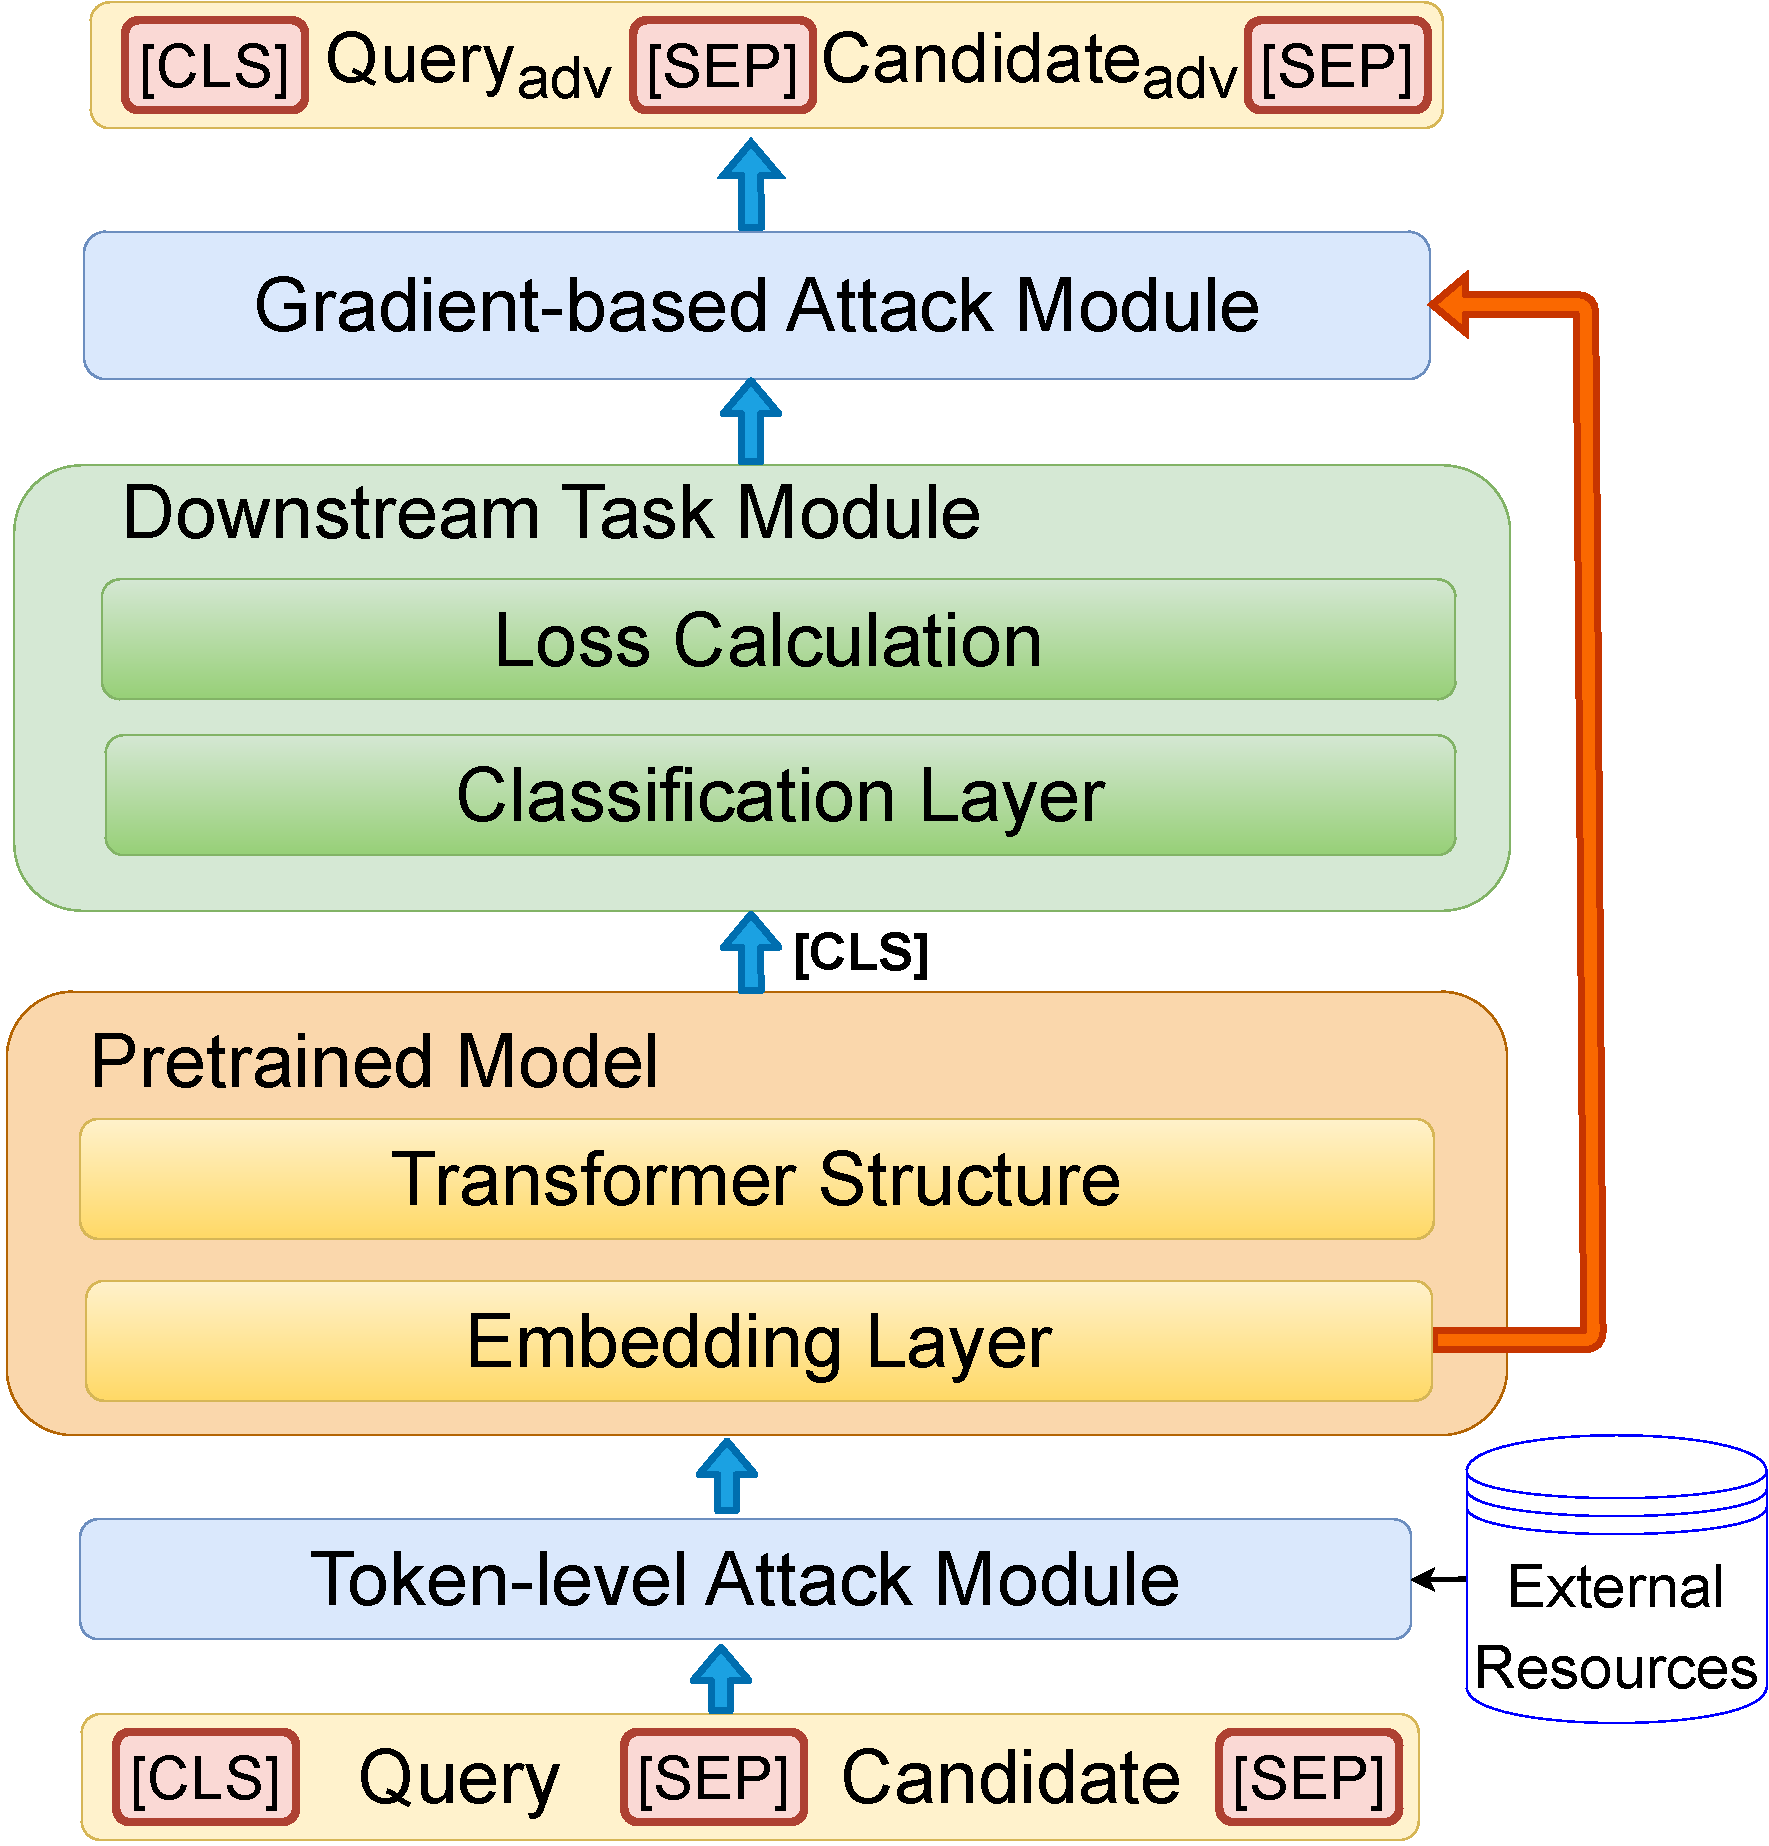
\includegraphics[width=0.5\columnwidth]{fig/fig3-2.pdf}
    \caption{对抗样本生成方法}
    \label{fig3-2}
\end{figure}

\textbf{词显著性排序} \quad 我们的词级攻击方法希望替换句子中对于模型重要的词汇,产生对模型较大的扰动,以达到在训练中提高模型语义提取能力和稳定性的效果。
我们利用词显著性来定义词汇的重要程度,每个词$x_i$的词显著性分数$I_{x_i}$计算如下:

\begin{equation}
    I_{x_i} = Loss(F(Input_{\not {x_i}}), y) - Loss(F(Input), y)
\end{equation}

其中,$Input_{\not {x_i}}$表示将输入序列中的词$x_i$进行遮蔽。
我们分别将序列中的每个词$x_i$逐个遮蔽,观察其对损失loss的影响。
如果该词对于句子的语义信息非常关键,将其遮蔽后,损失loss必然会有明显提升,反之loss则提升不明显。
我们以这样的方式作为词重要性的排序标准,对序列中的词重要性进行排序,对前N\%同义词替换。


\textbf{同义词替换攻击} \quad 对于每个需要替换的重要词$x_i$,我们需要选择合适的同义词进行替换,如果替换不慎,可能导致语义偏移,语法错误,甚至与原句语义完全相反。
首先,我们利用外部知识库WordNet\cite{miller1995wordnet}为$x_i$获取其同义词列表$L$。
接着,利用词性标注POS过滤$L$中词性与原词$x_i$不同的的候选单词,这一步是为了保证替换的同义词与原词词性相同,尽可能保证其语法的准确性。
此外,我们引入了反拟合嵌入空间(Counter-fitting embedding space)\cite{mrkvsic2016counte}作为词相似度的衡量方法。
我们将原词$x_i$和候选词$c_i$同时映射到反拟合嵌入空间,可以根据其在嵌入空间的余弦相似度,判断两者之间的语义是否相近。
我们设定阈值$p$为0.9,如果候选词中没有满足于该阈值要求,则放弃对$x_i$进行同义词替换,这是尽可能保证语义不发生偏移。
我们贪心地选择$L$中余弦相似度满足阈值要求的最高的候选词,对$x_i$进行替换。

\textbf{梯度攻击方法} \quad 

\subsection{自适应对抗训练方法}











% 单词、词块和短语等语言结构在答案选择过程中往往起到至关重要的作用。
% BERT能够有效的学习到词级的上下文语义表示,但是其无法在不同颗粒度的语言结构之间实现表示学习。
% 本章在BERT的基础上,对其输出进行不同粒度的n元语法卷积编码,借以获取句子中词块、短语等语义信息,
% 继而捕获多种粒度间的交互信息,使问题与答案之间的语义交互更加充分。
% 基于BERT的多粒度交互式推理模型(MIIN)如图~\ref{fig3-1}~左侧部分所示。

% \subsection{基于BERT的预训练编码}

% 给定问句$Q=\{q_1,\ldots,q_i,\ldots,q_n\}$以及答案段落$P=\{p_1,\ldots,p_j,\ldots,p_m\}$。
% 其中,n和m分别为其文本长度,$q_i$与$p_j$分别是问句的第i个单词和答案中第j个单词。
% 本章将问句Q和答案段落P构造成$S=[[CLS],Q,[SEP],P,[SEP]]$。
% 其中,$[CLS]$是分类标志符,$[SEP]$是用以区分输入中多个句子的分句符号。
% BERT将$S$的特征表示输入多层双向Transformer\cite{vaswani2017attention}构成的编码器中,
% 从而得到问题$Q$和候选答案$P$的联合编码表示T:$T=\{T_{[CLS]},T_{[Q]},T_{[SEP]},T_{[P]},T_{[SEP]}\}$。
% 值得说明的是,Transformer含有的多头自注意力机制,能够忽略词间距计算句子中所有词对之间的依赖关系。
% 因此,联合编码表示$T$中的分布特征已经得到了初步的注意力加权。此时,加权过程仅仅依赖词(Token)级的语义信息。

% \begin{figure}[!h]
    \centering
      \includegraphics[scale=1]{figure/fig3-1.pdf}
    \caption{基于BERT的多粒度交互编码模型架构}
    \label{fig3-1}
\end{figure}

% \subsection{多粒度卷积层}

% 本章使用卷积神经网络(CNN)对BERT输出的上下文词向量进行不同粒度的编码,
% 即分别对$T_{[Q]}=\{T_{[q_1]},T_{[q_2]},\ldots,T_{[q_n]}\}$以及对应的
% $T_{[P]}=\{T_{[p_1]},T_{[p_2]},\ldots,T_{[p_m]}\}$进行不同卷积核大小的卷积操作,
% 得到其对应的隐状态表示。编码过程如下所示:
% \begin{equation}
%     h_Q^k = CNN(T_{[Q]})
% \end{equation}
% \begin{equation}
%     h_P^k = CNN(T_{[P]})
% \end{equation}
% 其中,$h_Q^k$与$h_P^k$分别是对$T_{[Q]}$和$T_{[P]}$的不同粒度编码表示,
% $k$表示卷积核的大小为$k\times d$。
% 本章采用三个尺度的卷积核($k=\{1,\ 2,\ 3\}$),对应于三类$n$元语法(Unigram,Bigram和Trigram)。
% 从语法特征看,这三种粒度的卷积能够覆盖绝大部分词块、短语等情况,形成其独立的语义表示,有助于模型获取更加丰富的语义信息。

% \subsection{多粒度交互计算}

% 本章将问句与候选答案的多粒度编码表示输入到交互单元$\eta_k$,
% 获取k-gram粒度的交互特征向量$z^k$,$\eta_k$模块具体计算过程如下:
% \begin{equation}
%     e^k=H(h_Q^k,h_P^k)
% \end{equation}
% 其中,高阶交互函数$H$将$h_Q^k$与$h_P^k$都拓展成维度为$\mathbb{R}^{(n-k+1)\times(m-k+1)\times d}$的矩阵,
% 并将其对应位置的元素数值相乘,得到交互矩阵$e^k\in\mathbb{R}^{(n-k+1)\times(m-k+1)\times d}$。

% 其次,采用多层卷积操作从交互矩阵$e^k$提取特征,多层之间参数不共享,
% 并通过最大池化层,从卷积结果中过滤出强交互信号,具体交互计算如下:
% \begin{equation}
%     \widetilde{c_i^k}=ReLU(CNN(c_{i-1}^k))
% \end{equation}
% \begin{equation}
%     c_i^k=MaxPool(\widetilde{c_i^k})
% \end{equation}
% 其中,修正的线性单元(Rectified Linear Unit,简称ReLU)\cite{nair2010rectified}相比于传统的激活函数(如sigmoid\cite{han1995influence}),
% 能够有效的避免梯度爆炸问题。$\widetilde{c_i^k}$是对交互矩阵$e^k$第$i$次卷积的结果,
% $c_i^k$是$\widetilde{c_i^k}$经过最大池化的结果($c_0^k=e^k$)。

% 最后,本章将提取到的特征矩阵$c^k$展开得到特征向量,
% 并将其输入全连接网络(Fully Connected Network,简称FC),
% 对拼接的多粒度特征向量进行推理计算得到最终高度聚合的交互特征向量$z^k$,具体过程如下:
% \begin{equation}
%     z^k=W_z^k(flatten(c^k))+b_z^k
% \end{equation}
% 其中,$W_z^k$和$b_z^k$是可训练参数,函数$flatten()$用以将交互矩阵$c^k$按照维度展开拼接为1维向量表示,特征$z^k\in\mathbb{R}^{1\times d}$。

% \subsection{答案相关性预测}

% 输出层将不同粒度的交互特征向量$z^k=\{z^1,z^2,z^3\}$与BERT分类特征向量$T_{[CLS]}$拼接得到综合性交互表示$o\in\mathbb{R}^{4\times d}$,
% 并将其输入到全连接网络中,并计算问句与答案段落的相关性分数。
% 全连接网络在反向传播的过程中,不断根据预测分数与实际结果之间的差异更新其参数值,以此自动察觉不同粒度信息的权重差异。
% 具体过程如下:
% \begin{equation}
%     o=[z^1;z^2;z^3;T_{[CLS]}]
% \end{equation}
% \begin{equation}
%     r=W_oo+b_o
% \end{equation}
% 其中,$W_o$与$b_o$为可训练参数,感知机最终输出的标量$r$即为最终相关性得分,分数高低与相关性成正比。

% \subsection{损失函数及子句损失策略}

% 本章采用Pairwise方法训练与学习答案选择任务,旨在使正样本与问题相关性得分明显高于负样本(正样本表示与问题相关的答案段落,负样本表示与问题不相关或者相关性较低的答案段落)。
% 具体而言,对于一个问题Q,Pairwise方法构造正负样本对$(Q,P^+)$与$(Q,P^-)$,并通过合页损失函数进行学习。
% 其中,$P^+$为正样本,$P^-$为负样本(若问题$Q$的正样本有$n$个,负样本有$m$个,则共有$n\ast m$个Pairwise正负样本对),正负样本答案段落合页损失计算如下:
% \begin{equation}
%     \mathcal{L}(P)=max(0,\varepsilon+r_{P^-}-r_{P^+})
% \end{equation}
% 其中,$r_{P^+}$和$r_{P^-}$分别是正负样本的相关性分数,$\varepsilon$是正负样本分数差值的阈值,函数$max()$表示从给定参数中选取最大值。

% 此外,本章在损失函数中加入子句损失,用于提升答案段落中相关程度较高的子句在答案选择过程中的作用。
% 如图~\ref{fig3-1}~所示,模型在判别答案整体与问题相关性的同时,对所有子句相关性作出预测,
% 把排名靠前的几个子句的损失添加到最终损失中,以提升关键子句的权重。
% 其中,子句与问题之间的相关性标签取决于其所属答案段落的标签。
% 若正样本$P^+=(s^{1+},\ldots,s^{i+},\ldots)$,负样本$P^-=(s^{1-},\ldots,s^{j-},\ldots)$,
% 其中$s^{i+}$表示正样本答案段落中第$i$句文本,$s^{j-}$表示负样本中第$j$句文本。
% 正负样本子句合页损失计算过程分别如下:
% \begin{equation}
%     \mathcal{L}(s^{i+})=max(0,\varepsilon+r_{s^{i+}}^--r_{s^{i+}}^+)
% \end{equation}
% \begin{equation}
%     \mathcal{L}(s^{j-})=max(0,\varepsilon+r_{s^{j-}}^+-r_{s^{j-}}^-)
% \end{equation}
% 其中,$r_{s^{i+}}^+$与$r_{s^{i+}}^-$分别为正样本中第$i$个子句与问题相关性的二分类正向分数与负向分数,
% $r_{s^{j-}}^+$与$r_{s^{j-}}^-$分别为负样本中第$j$个子句与问题相关性的二分类正负向分数。
% 通过设置超参数$sent=N$,分别从正负样本中提取与问题相关性最高的$N$个子句计算损失,
% 用这些子句损失的平均值作为该正负样本对的子句总损失。
% 总体损失则等于合页损失与子句损失的“零和”折损,计算如下:
% \begin{equation}
%     \mathcal{L}_N(s)=mean(\sum_{i}^{N}\mathcal{L}(s^{i+})+\sum_{j}^{N}\mathcal{L}(s^{j-}))
% \end{equation}
% \begin{equation}
%     \mathcal{L}=
%     \begin{cases}
%         \mathcal{L}(P), \ \ &\mathcal{L}_N(s)=0\\
%         \mathcal{L}(P)\mathcal{L}_N(s),\ \ &\mathcal{L}_N(s)>0
%     \end{cases}
% \end{equation}
% 其中,$\mathcal{L}(s^{i+})$和$\mathcal{L}(s^{j-})$分别为正负样本子句合页损失,$\mathcal{L}_N(s)$表示子句总损失,$\mathcal{L}(P)$表示正负样本答案段落合页损失,$\mathcal{L}$表示模型的总损失。

\section{实验及结果分析}

\subsection{数据集、评价方法与超参设置}
本章在WPQA数据集上进行实验,数据集的详细介绍见~\ref{2.2 语料资源概述}~小节。
实验采用平均化精度均值MAP和
平均化倒数排序MRR评价模型的排序能力,具体介绍见~\ref{2.3 性能评价指标}~小节。
本章的基线模型为BERT-base模型(12-layer, 768-hidden, 12-heads),总参数量约为110M。
输入模型的问题与答案的最大长度限制分别为40和400。
交互层使用2层卷积池化网络提取特征,卷积与最大池内核大小均为$2\times2$。
模型在训练阶段batch\_size设置为10,优化函数的学习率(learning\_rate)设置为3e-6,
优化函数中的epsilon\cite{rutherford2002lecture}设置为1e-8。子句优化策略中子句数量sent设置为2,子句最大长度限制为55。
合页损失阈值$\varepsilon$设置为1。

\subsection{前沿方法介绍}

为了验证本章所提方法的有效性,本章在WPQA数据集上与现有方法进行比较,并对其结果进行分析。
除了经典的统计模型BM25\cite{robertson1994some}和
TF-IDF(Term frequency–inverse document frequency,简称TF-IDF)\cite{ramos2003using}以外,
本章还与如下基于深度学习的前沿方法进行了比对:
\begin{itemize}
    \item \textbf{Att-BiLSTM}(Tan et al., 2016)\cite{tan2016improved}
    将注意力机制与BiLSTM (Bi-directional Long Short-Term Memory,简称BiLSTM)结合,
    使模型学习到的答案向量包含更多与问题相关的信息。
    \item \textbf{AP-BiLSTM}(Santos et al., 2016)\cite{santos2016attentive}
    在传统BiLSTM答案选择模型基础上,加入注意力层与多样化的池化层,使用行最大池与列最大池
    分别从问题与答案的交互矩阵中提取交互特征,从而使得问题特征向量中包含答案信息,答案特征向量中包含问题信息。
    \item \textbf{LW-BiLSTM}(Rücklé et al., 2017)\cite{ruckle2017representation}
    与其他基于注意力的模型相反,该方法不依赖于问题与答案的相关性,假设问题与候选答案相对独立,
    使用BiLSTM模块学习答案中单词的权重。
    \item \textbf{CA-Wang}(Wang et al., 2016)\cite{parikh2016decomposable}
    首次将Parikh等提出的Compare-Aggregate框架应用到匹配任务中,分析了多种Compare方法对模型的影响。
    \item \textbf{COALA}(Rücklé et al., 2019)\cite{ruckle2019coala}
    仅关注答案对问题的影响,使用最大池以代替注意力机制和传统的神经网络聚合层从相似度矩阵中提取问题相关特征,并使用平均化运算操作得到最终结果。
    \item \textbf{MICRON}(Han et al., 2019)\cite{han2019micron}
    使用多种n-gram卷积对问题和答案分别进行上下文编码,将其不同粒度的编码结果交叉交互,
    利用多粒度交互从问题与答案文本中提取相关信息。
    \item \textbf{BERT-PR}(Xu et al., 2019)\cite{xu2019passage}
    将预训练模型BERT应用到段落级答案选择任务中,
    同时考虑答案段落在缺少标注信息情况下的场景,使用BM25、TF-IDF等方法的投票结果作为答案段落的标签信息。
    \item \textbf{BERTlets}(Mass et al., 2019)\cite{mass2019study}
    使用BERT处理段落级答案选择任务,并通过实验分析了不同学习方式(Pointwise与Pairwise)
    以及不同文本长度限制对模型的影响。
\end{itemize}

\subsection{对比实验及分析}

表~\ref{table3-2}~列出了上述方法和本章所提方法(BERT-MIIN)在WPQA数据集上的性能。
结果显示,BERT-MIIN的MAP值和MRR值均达到最高。
经典的统计模型BM25和TF-IDF依靠特征工程的方法处理句间关系,缺乏语义理解能力,无法有效处理问题与答案之间的语义关系。
Att-BiLSTM等传统神经网络模型受到数据集大小的限制,难以充分学习到句子的语义信息,在文本较长的答案选择任务中表现不佳。
COALA模型和MICRON模型部分采用算术运算的方式代替神经网络进行交互与聚合,大大减少可训练参数量,
从而通过较少的训练数据即可取得较优效果,在一定程度上缓解了数据量限制的问题。
预训练语言模型BERT通过自监督方式在海量语料的基础上进行训练,其词向量包含丰富的上下文信息,
从而使得BERT-PR及BERTlets模型性能大幅上升。
但是,BERT-PR与BERTlets仅使用BERT的分类特征作为结果的唯一依据,且并未考虑多粒度的语义信息,从而性能低于BERT-MIIN。

\begin{table}
    \caption{模型性能对比}
    \centering
    \newcommand{\tabincell}[2]{\begin{tabular}{@{}#1@{}}#2\end{tabular}}
    \begin{tabular}{l|c|c}
    \toprule[0.7pt]
    \textbf{模型\qquad\qquad\qquad\qquad\ } & \textbf{\enspace MAP (\%)\enspace} & \textbf{\enspace MRR (\%)\enspace  } \\
    \midrule[0.7pt]

    BM25 & 53.73 & 62.58 \\
    TF-IDF & 39.92 & 46.38 \\
    \midrule[0.4pt]
    Att-BiLSTM & 47.04 & 54.36 \\
    AP-BiLSTM & 46.98 & 55.20 \\
    LW-BiLSTM & 47.56 & 54.33 \\
    CA-Wang & 48.71 & 56.11 \\
    COALA & 60.58 & 69.40 \\
    MICRON & 63.00 & 71.03 \\
    BERT-PR & 73.55 & 80.87 \\
    BERTlets & 73.60 & 81.00 \\
    \midrule[0.4pt]
    BERT(baseline) & 73.70 & 81.02 \\
    BERT-IIN & 74.02 & 81.33 \\
    BERT-MIIN & 74.84 & 82.04 \\
    \textbf{BERT-MIIN$_{sent2}$} & \textbf{75.20} & \textbf{82.21} \\
    \bottomrule[0.7pt]
    \end{tabular}
    \label{table3-2}
\end{table}

值得注意的是,BERT-IIN模型对词向量进行2-grams卷积编码(非多粒度),
以此获取问题与答案段落的局部上下文信息进行交互,其性能相较于基线有所提升。
BERT-MIIN使用多种卷积对词向量进行多粒度编码,获取到不同粒度的局部上下文信息,
并分别进行句间交互,使得问题与答案之间的交互更加充分。
由表~\ref{table3-2}~可见,BERT-MIIN的MAP和MRR指标明显高于仅采用单一粒度卷积交互的BERT-IIN,
且相较于基线分别提升了1.14\%和1.02\%。
BERT-MIIN$_{sent2}$在BERT-MIIN基础上加入了子句损失策略,
对答案段落中与问题最相关的两个子句计算损失,这有助于神经网络模型敏感地感知关键的关联语句,
并避免冗余信息对关联性判断的误导,使得MAP和MRR的性能值得以进一步提升。



\subsection{显著性分析}

实验使用显著性检验确保实验结果非偶然性,即分别计算BERT-MIIN和BERT-MIIN$_{sent2}$
对比BERT在WPQA数据集上MAP指标和MRR指标的P-value值。
P-value小于0.05表示结果存在显著差异,否则差异不显著。
由表~\ref{table3-3}~可见,本章提出的方法在统计上存在显著提升。

\begin{table}[h]
    \caption{显著性分析结果}
    \centering
    \newcommand{\tabincell}[2]{\begin{tabular}{@{}#1@{}}#2\end{tabular}}
    \begin{tabular}{l|c|c}
    \toprule[0.7pt]
    & \enspace \textbf{BERT-MIIN} \enspace& \enspace \textbf{BERT-MIIN$_{sent2}$} \enspace\\
    \midrule[0.7pt]

    MAP\qquad\quad & 0.030 & 0.018 \\
    MRR & 0.047 & 0.038 \\

    \bottomrule[0.7pt]
    \end{tabular}
    \label{table3-3}
\end{table}

\subsection{子句损失策略的性能分析}

本章使用BERT(与答案段落排序共享参数)对子句进行相关程度排序,子句的最大长度限制为55。
超参数$sent=N$表示取与答案段落中问题最相关的前$N$个子句计算损失,图~\ref{fig3-2}~通过实验分析sent取值对模型性能的影响。

\begin{figure}[h]
    \centering
      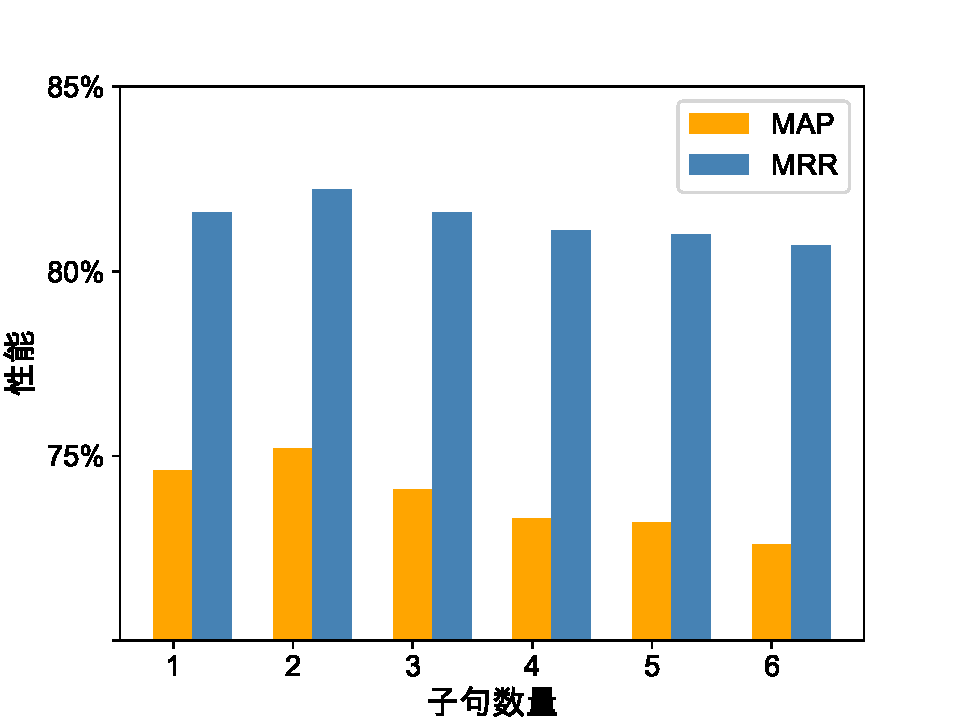
\includegraphics[scale=0.5]{figure/fig3-2.pdf}
    \caption{不同子句数量限制性能对比}
    \label{fig3-2}
\end{figure}

由图~\ref{fig3-2}~可见,当子句数量限制为2时,模型性能达到最高,
MAP和MRR值分别为75.20\%、82.21\%。实验结果表明,
部分数据的答案段落中与问题密切相关的子句往往只有1~2句。
为了验证模型对子句排序结果可信度,本章从WPQA测试集中随机取出200个问题及其候选答案段落组,
在候选答案组中取其中一个正样本(即相关答案段落)进行人工标注,与问题密切相关的子句标注为1,相关程度较低的子句标注为0。
最终共计标注1,200条子句数据,其中,与问题密切相关的子句有288条,具体信息如表~\ref{table3-4}~所示。

\begin{table}[h]
    \caption{子句测试数据统计}
    \centering
    \newcommand{\tabincell}[2]{\begin{tabular}{@{}#1@{}}#2\end{tabular}}
    \begin{tabular}{l|l|l}
    \toprule[0.7pt]
    & \;\textbf{数量} & \;\textbf{平均长度} \\
    \midrule[0.7pt]

    问题 & \;200 & \;9.78\\
    答案(子句)\quad\; & \;1,200\; & \;24.46\\
    相关答案 & \;288 & \;27.41\\

    \bottomrule[0.7pt]
    \end{tabular}
    \label{table3-4}
\end{table}

表~\ref{table3-5}~列出了在WPQA数据集上训练后,模型对人工标注数据排序的性能。
加入子句损失策略后的BERT-MIIN$_{sent2}$对子句的排序性能优于BERT和BERT-MIIN。
实验结果表明,子句损失策略不仅提升了模型在段落级答案选择任务上的性能,
同时能够对答案段落中的子句进行较为精准的相关度排序,具有一定的参考和应用价值。

\begin{table}[h]
    \caption{子句测试数据集排序性能}
    \centering
    \newcommand{\tabincell}[2]{\begin{tabular}{@{}#1@{}}#2\end{tabular}}
    \begin{tabular}{l|c|c}
    \toprule[0.7pt]
    \textbf{模型} & \enspace \textbf{MAP} \enspace& \enspace \textbf{MRR} \\
    \midrule[0.7pt]

    BERT & 82.99 & \enspace 86.02 \\
    BERT-MIIN & 84.33 & \enspace 86.53 \\
    \textbf{BERT-MIIN$_{sent2}$}\quad\; & \textbf{85.18} & \enspace \textbf{87.26} \\

    \bottomrule[0.7pt]
    \end{tabular}
    \label{table3-5}
\end{table}

\section{本章小结}

本章提出了一种多粒度交互推理模型BERT-MIIN,证明了该模型可以有效地捕获“问题与答案”之间的精细语义信息,并主动关注答案中的关键句子。
实验证明,本章提出的模型和策略在非事实性问答数据集上性能均有提升。
下一章将尝试从“问题与问题”之间语义匹配角度出发,优化问题复述识别模型的表现,
提高问答匹配技术的实际应用能力。

% 本章将进一步完善BERT-MIIN在答案选择任务中的应用,实现更深层次的语义理解与交互。
% 同时,尝试将该方法应用到其他文本匹配领域中。




\chapter{面向问题复述识别的定向数据增强方法}

上一章采用多粒度卷积交互推理方法强化了模型对“问题与答案”之间的精细语义感知能力,其有利于优化问答场景下相关答案的召回质量。
本章集中研究问题复述识别任务中“问题与问题”之间的精细语义关系,用以提高问答场景下同义问题(已知答案)的召回精度。
% 该任务旨在召回“同质异构”的问句对子(语义相同表述迥异的问句),
% 其可被降解为面向自然问句的二元分类问题,即对输入的问句对子进行“复述”和“非复述”的二相判别。
现有预训练语言模型被广泛应用于自然语言的语义编码,并取得了显著的性能优势。
然而,其优势并未在问题复述的求解中得到充分的体现,原因在于:
1)预训练语言模型善于生成通用的语义表示,对特定任务中精细的语义表示需求并不敏感;
2)复述样本的“是与非”往往取决于极为微妙的语义差异。
微调预训练语言模型成为提高其任务适应性的关键步骤,但其极大依赖训练数据的数量(多样性)与质量(可靠性)。
为此,本章提出一种基于生成模型的定向数据增强方法(DDA)。
该方法能够利用诱导标签对神经生成网络进行引导,借以自动生成多样的复述和非复述的增强样本,促进训练数据的自动扩展。
此外,本章设计了一种多模型集成的标签投票机制,并用其修正增强样本的潜在标签错误,以此提高扩展数据的可靠性。
在中文问题复述数据集LCQMC上的实验结果证明,与传统数据增强方案相比,本章方法生成的样本质量更高,且语义表达更加多元化。
下面将详细介绍本章的研究动机、相关方法以及具体的实验论证。

\section{引言}

问题复述识别是问答匹配研究领域中的重要任务之一,
其旨在判断两个自然问句的语义是否等价或具有较高相似度,即对输入的问句对子进行“复述”和“非复述”的二相判别。
如表~\ref{table4-1}~中{\kai“移动号码如何转为电信号码?”}与{\kai“能把移动转为电信号码吗?”},这两个问句表达的意思完全相同,为复述关系(标签为1表示复述关系)。
当前,问题复述识别技术已经被广泛应用到多种实际场景中,如:搜索引擎、社区问答以及智能客服等。
深度神经网络的发展推动了复述识别等自然语言处理(Natural Language Processing,简称NLP)的研究。
其中,BERT\cite{devlin2018bert}等基于大规模语料预训练的语言模型能够复用并微调其注意力和联合编码机制,
使其具有适应性更强的文本语义特征提取和交互能力,在问题复述识别等任务中表现出色。

\begin{table}[h]
    \caption{LCQMC及增强数据示例}
    \centering
    \newcommand{\tabincell}[2]{\begin{tabular}{@{}#1@{}}#2\end{tabular}}
    \begin{tabular}{lllcc}
    \toprule[0.7pt]
    \textbf{样本来源} & \textbf{问题1} & \textbf{问题2}& \textbf{标签}& \textbf{合格?} \\
    \midrule[0.7pt]

    LCQMC & \multirow{4}{*}{移动号码如何转为电信号码?} & 能把移动转为电信号码吗? & 1 & Y \\
    BT & & 如何将手机号码转换为电信号码? & 1 & N \\
    EDA &  & 移动号码转为电信号码? & 1 & Y \\
    DDA &  & 电信号码可以改为移动号码吗? & 0 & Y \\
    \midrule[0.4pt]
    LCQMC & \multirow{4}{*}{什么牌子空调最好?} & 什么牌子空调扇最好? & 0 & Y \\
    BT &  & 哪个牌子的空调最好? & 1 & Y \\
    EDA &  & 什么牌子的空气调节最好? & 1 & N \\
    DDA &  & 空调什么牌子最好? & 1 & Y \\


    \bottomrule[0.7pt]
    \end{tabular}
    \label{table4-1}
\end{table}

现代神经网络模型在训练过程中往往需要大量的标注数据进行学习。
但是,标注给定句子的复述句需要消耗庞大的人力成本,这导致了当前的复述识别数据集往往规模有限。
这种普遍的数据稀缺性问题对模型的泛化性和鲁棒性提出了极大的挑战。
当前,数据增强策略(Data Augmentation)是扩充数据样本规模的一种有效方法,在一定程度上能够缓解数据因素对模型学习能力的制约。
Wei等提出简单数据增强策略EDA\cite{wei2019eda},
其在原始样本的基础上采用随机删除、插入、交换、同义词替换四种操作构造增强样本。
Yu等采用的回译策略BT\cite{yu2018qanet}将英文样本翻译为法文,然后再翻译回英文,
期望样本在保持原意的前提下能够增加、删除、修改原词或重新组织原句。
如表~\ref{table4-1}~所示(Y表示样本质量合格,N表示样本质量不合格),尽管EDA和BT策略能够高效地扩充数据数量,但是其仅能构造与原样本语义相同的数据,
并且无法保证构造样本的语法正确性和标签一致性(即样本不合格),这些包含错误知识的数据对模型产生负面影响。

本章提出一种基于生成模型的定向数据增强策略(Directional Data Augmentation,简称DDA),
在预训练语言模型UNILM(Unified Language Model)\cite{bao2020unilmv2}的输入中添加定向标签,使其生成期望的复述句或非复述句。
UNILM强大的生成能力能有效降低文本的语法错误率。
此外,为了进一步提高数据质量,确保问题对的标签真实性,本章设计了一种标签修正策略,对新生成的文本对的标签进行纠错。
从表~\ref{table4-1}~可以看出,相比于EDA等方案,UNILM语言模型产出的样本质量更高,样本难度更大。
同时,DDA策略仅使用定向标签约束生成样本的语义,使其具有多元化变动,更加符合真实语言环境,有助于提高模型的鲁棒性。
本章在LCQMC\cite{liu2018lcqmc}中文问题复述数据集上进行实验,并在多个基线模型上验证DDA策略的有效性。
本章的主要贡献有:

\begin{enumerate}
    \item 
    提出一种通用的定向数据增强方案,能够大规模地产出高质量、多元化的“复述”与“非复述”的数据样本。
    \item 
    基于中文问题复述语料LCQMC构造公开增强数据集LCQMC$_{DDA}$,实验表明其对基线模型的性能及泛化能力具有普遍的提升作用。
\end{enumerate}

本章的组织形式如下:第1节为引言部分;第2节详细介绍本章所提出的定向数据增强方法;第3节对方法进行实验验证及分析;第4节总结本章并展望未来工作。


\section{系统框架及主要研究内容}

\subsection{总体结构}

数据规模与质量对于模型的学习过程往往起到至关重要的作用。尤其在小规模数据集上,数据增强策略能够为模型带来巨大收益。
本章基于UNILM语言模型生成定向增强样本,同时采用多判别器集成投票策略修正样本标签,最终形成高质量的问题复述识别样本。

\subsection{定向问题生成}

本章使用LCQMC数据训练定向问题生成模型。
LCQMC中的样本是由问题$Q$、问题$Q^t$以及标签$L$三者组成的三元组$(Q,Q^t,L)$,
其中$L\in\{0,1\}$表示$Q$与$Q^t$是否为复述关系。
本章使用预训练语言模型UNILM构建定向问题生成模型。
UNILM在BERT的自编码MLM(Masked Language Model)\cite{taylor1953cloze}任务基础上,
加入部分自回归的掩码策略,使得模型不仅具有捕获上下文语义能力,
而且能够对连续的掩码部分进行整体预测,增强模型词块、词组的理解和生成能力。

传统的问题复述生成模型利用某一给定源问题$Q$,生成与源问题语义一致的复述问句$Q^\prime$。
本章提出的定向问题生成策略,在输入中加入定向引导标签$L\in\{0,1\}$,
使其引导模型在不同语义方向上对问句做微小改动,强化模型的定向生成能力。
当$L=1$时,期望生成与源问题$Q$语义一致的复述问题$Q^\prime$;
当$L=0$时,期望生成与源问题$Q$语义不一致,但两者之间字面高度相似的非复述问题$Q^\prime$,
使得问题复述判别模型容易将$Q$与$Q^\prime$误判为语义一致的复述问题对。
最终,生成模型的输入如下:
\begin{equation}
    X=\{[CLS],L,[SEP],Q,[SEP]\} \notag
\end{equation}
其中,$[CLS]$是包含整个输入部分语义信息的标志,$[SEP]$是用以区分输入中多个成分的分隔符号。
UNILM将$X$的特征表示输入多层双向Transformer\cite{vaswani2017attention}编码块构成的编码器,
从而得到问题$Q$和定向引导标签$L$的联合编码表示$T$:
\begin{equation}
    T=\{T_{[CLS]},T_{[L]},T_{[SEP]},T_{[Q]},T_{[SEP]}\} \notag
\end{equation}
值得说明的是,Transformer含有多头自注意力机制。
因此,联合编码表示$T$中的分布特征已经得到注意力加权,
此时,$T_{[Q]}$中已经充分融合了定向标签$L$的特征信息。
最终,将联合编码表示$T$作为生成目标问句$Q^\prime$的隐状态逐步生成目标问句$Q^\prime$,
将其与真实目标问句$Q^t$进行拟合,其损失计算公式如下:
\begin{equation}
    \mathcal{L}_G({q_i}^\prime)=-logP({q_i}^\prime\ =\ {q_i}^t\ |\  L,Q,{q_{<i}}^t,{q_i}^\prime)
\end{equation}
其中,$\mathcal{L}_G$表示负对数似然损失。
${q_i}^\prime$和${q_i}^t$分别是生成的目标问题$Q^\prime$与真实目标问句$Q^t$中第$i$个词。

通过上述训练方式,模型在生成时能捕获到定向诱导标签、源问题以及目标问题当前时间步之前的信息,
使得模型在预测阶段能够参考定向诱导标签生成期望的复述或非复述问句。
如表~\ref{table4-1}~所示,源问题为{\kai“什么牌子空调最好?”},
当给定诱导标签$L\ =\ 1$时,模型可定向生成与源问题语义一致的问句{\kai“空调什么牌子最好?”};
当给定源问题{\kai“移动号码如何转为电信号码?”}及定向诱导标签$L\ =\ 0$时,
模型可生成与源问题语义不同却字面相似的问句{\kai“电信号码如何转为移动号码?”}。

本章使用LCQMC复述数据集进行实验,利用模型生成一批与原样本标签相反的增强数据。
本章将LCQMC三元组$(Q,Q^t,L)$中的源问题$Q$以及标签的反置$!L$(当$L=0$时,$!L=1$;当$L=1$时,$!L=0$)作为定向生成模型的输入,从而得到新的增强样本$(Q,Q^\prime,!L)$。
最终,本章在LCQMC的23.8万样本的基础上,扩充了一批标签相反的增强样本,
经过简单的规则过滤(剔除$Q^\prime$与$Q$完全一致或过于相近的样本),共保留16.3万条有效样本。

\subsection{标签修正}

定向生成模型能够将定向诱导标签和问句的特征表达相融合,生成语义与诱导标签走向一致的目标问句。
本章仅采用定向标签进行语义诱导,其包含的信息内容简单,对模型限制的较少且使用代价微小,使模型生成的问句更加具有多样性。
但由于没有更多的外部知识引导定向问题的语义特征,这种方法导致增强样本中仍存在一些不满足定向诱导标签语义要求的问句。
例如,表~\ref{table4-4}~中的源问题{\kai“长方体的底面积怎么求?”},给定诱导标签$1$时,模型生成的问句{\kai“长方体的面积怎么求?”}语义已经发生偏转,该样本实际上是标签为$0$的非复述样本。
因此,本章采用人工标注方法,从增强样本中标注出1,000条作为增强样本测试集,用以验证增强样本的标签与人工标注标签的一致率,
标注结果显示样本标签一致率为70.2\%。

对此,本章设计了一种基于多判别模型的集成投票方法,用以修正增强样本的标签。
本章使用BERT$_{base}$\cite{devlin2018bert}、RoBERTa$_{large}$\cite{liu2019roberta}和MacBERT$_{large}$\cite{cui2020revisiting}三种预训练语言模型在LCQMC数据集上进行微调,以此作为问题复述判别器基线。
本章将源问题$Q$以及目标问题$Q^t$作为判别器的输入,预测两者之间是否为复述关系$L^\prime$,
并将其与真实标签$L$进行拟合。具体的损失计算公式如下:
\begin{equation}
    \mathcal{L}_D(L,L^\prime)=-Llog(p)-(1-L)log(1-p)
\end{equation}
其中,$\mathcal{L}_D$表示二分类交叉熵损失,$p$为样本为复述关系的概率。
本章使用以上三个判别器对源问题$Q$与生成的目标问题$Q^\prime$进行预测,
若两个或两个以上模型预测结果与定向标签相符合,则将定向标签作为最终标签。
否则,将三个模型预测的复述概率均值$p>=\alpha$的样本修正为复述问题对,即标签为1;
将复述概率均值$p<=\beta$的样本修正为非复述问题对,即标签为0($score\in[0,1]$)。
通过在LCQMC$_{DDA}$测试集合上不断调试(详见~\ref{4.3.3 标签修正策略分析}~节),
本章发现当$\alpha$取值0.92且$\beta$取值0.5时,修正后的样本标签与$L’$人工标注的标签最为接近,
标签一致率约95\%,共将约3.1万条样本修正为复述样本,9千条样本修正为非复述样本。
本章将标签修正后的16.3万条样本作为增强数据集LCQMC$_{DDA}$,用于优化问题复述识别模型在目标数据集上的性能以及鲁棒性。


\section{实验及结果分析}

\subsection{数据集与评价方法}

本章在中文问题复述数据集LCQMC上进行实验,验证DDA方法的有效性,数据集的详细介绍见~\ref{2.2 语料资源概述}~小节。
本章提出的DDA数据增强策略,针对LCQMC数据集构造了对应的增强数据集LCQMC$_{DDA}$。
其样本格式与LCQMC完全一致,共包含约16.5万个问题对。
表~\ref{table4-2}~列出了LCQMC$_{DDA}$增强数据集的统计信息。
本章实验采用准确率Acc评价模型的二元分类能力,具体介绍见~\ref{2.3 性能评价指标}~小节。

\begin{table}
    \caption{LCQMC$_{DDA}$数据统计表}
    \centering
    \newcommand{\tabincell}[2]{\begin{tabular}{@{}#1@{}}#2\end{tabular}}
    \begin{tabular}{l|l|l|l}
    \toprule[0.7pt]
    & \;\textbf{总计} & \;\textbf{正样本} & \;\textbf{负样本} \\
    \midrule[0.7pt]

    训练集\quad\; & \;163,158\; & \;68,968\; & \;94,190 \\
    测试集 & \;1,000 & \;465 & \;535 \\
    \bottomrule[0.7pt]
    \end{tabular}
    \label{table4-2}
\end{table}

\subsection{基线模型与超参设置}

\textbf{(一) 定向问题生成模型}

本章基于UNILM(v2)模型架构(12-layer,768-hidden,12-heads)进行微调。
UNILM(v2)采用部分自回归的掩码策略,使模型能对连续的mask部分进行整体预测,增加了模型对词块的理解和生成能力。
输入的源问句与目标问句最大长度限制均为35。
模型在训练阶段batch\_size设置为64,优化函数的学习率(leraning\_rate)设置为2e-5,
优化函数中的epsilon\cite{rutherford2002lecture}设置为1e-8。

\textbf{(一) 问题复述判别模型}

本章使用BERT$_{base}$、RoBERTa$_{large}$和MacBERT$_{large}$三种预训练语言模型作为问题复述识别任务的判别模型:
\begin{itemize}
    \item \textbf{BERT$_{base}$}(Devlin et al., 2018)\cite{devlin2018bert}
    使用Transformer作为主要架构,能更彻底的捕获文本中的双向关系。
    其在海量语料上使用语言掩码任务(Mask Lanauage Model)以及句对预测任务(Next Sentence Prediction)
    进行自监督训练,学习蕴含上下文的动态特征表达。
    \item \textbf{RoBERTa$_{large}$}(Liu et al., 2019)\cite{liu2019roberta}
    对比BERT模型而言,其参数量、语料规模更大,并且采用动态掩码策略使训练语料的利用的更加充分,在NLP任务中的表现更加出色。
    \item \textbf{MacBERT$_{large}$}(Rutherford et al., 2020)\cite{cui2020revisiting}
    是在RoBERTa基础上改进的中文语言模型,其借助近义词工具(Synonyms)\footnote{https://github.com/chatopera/Synonyms}获取掩码词的近义词或同义词进行替换,
    能够缓解预训练与微调(fine-tune)阶段的误差,以及提高模型的鲁棒性。
\end{itemize}

本章判别模型输入问题对的最大长度限制为65。模型在训练阶段batch\_size设置为64,优化器的学习率设置为5e-6,
优化函数中的epsilon设置为1e-8。

\subsection{定向数据增强(DDA)实验分析}

为了验证本章方法的有效性,本章将LCQMC$_{DDA}$作为增强数据扩充到LCQMC数据集中,并将其对判别模型的增强结果进行分析。
本章通过数据增强技术探索DDA策略对这些基线模型的作用。
此外,为了从多种角度评判DDA策略为问题复述识别模型带来的泛化性及鲁棒性综合收益,
本章还在公开的问题复述鲁棒性评测数据CQM$_{robust}$(详见章节\ref{5.point3})上进行评估。
相较于传统数据集,CQM$_{robust}$中蕴含多种中文语言特征,且样本迷惑性较强,对判别模型的挑战更大。并且该测试集中的样本均来源于百度搜索中的真实问题,与真实世界中的样本分布更接近。
因此,其实验结果更能反映DDA策略产出数据的真实性和多样性。

\begin{table}
    \caption{DDA数据增强试验结果}
    \centering
    \newcommand{\tabincell}[2]{\begin{tabular}{@{}#1@{}}#2\end{tabular}}
    \begin{tabular}{l|l|cc|c|c}
    \toprule[0.7pt]
    \multirow{2}{*}{\textbf{模型}} & \multirow{2}{*}{\enspace \textbf{训练数据\enspace }} & \multicolumn{2}{c|}{\textbf{LCQMC}} & \;\textbf{LCQMC$_{DDA}$}\; & \;\textbf{CQM$_{robust}$}\; \\
    \cline{3-6}
    & & \enspace Dev\; & \; Test\enspace & Test & Test\\
    \midrule[0.7pt]

    \multirow{3}{*}{BERT$_{base}$} & \enspace LCQMC & 89.1 & 86.5 & 83.5 & 71.6 \\\cline{2-6}
    &\enspace + DDA$_{noise}$ & 84.7 & 83.4 & 77.4 & 70.6 \\
    &\enspace \textbf{+ DDA} & \textbf{90.2} & \textbf{87.7} & \textbf{86.9} & \textbf{74.4} \\
    \midrule[0.4pt]
    \multirow{2}{*}{RoBERTa$_{large}$} & \enspace LCQMC & 90.5 & 88.0 & 84.6 & 75.9 \\
    &\enspace \textbf{+ DDA} & \textbf{90.9} & \textbf{88.6} & \textbf{87.2} & \textbf{77.8} \\
    \midrule[0.4pt]
    \multirow{2}{*}{MacBERT$_{large}$\quad} & \enspace LCQMC & 90.9 & 88.2 & 84.6 & 78.0 \\
    &\enspace \textbf{+ DDA} & \textbf{91.2} & \textbf{89.5} & \textbf{87.0} & \textbf{79.2} \\
    \bottomrule[0.7pt]
    \end{tabular}
    \label{table4-3}
\end{table}

表~\ref{table4-3}~列出了上述判别模型在数据增强前后的实验结果。
由表可知,DDA增强数据不仅提高了模型在LCQMC测试数据上的表现,也增强了模型应对领域外复杂样本的能力,
其在CQM$_{robust}$上的性能平均提升了约2\%。
此外,在基线模型中,MacBERT针对中文特点进行相似词掩码间接优化模型泛化能力,因此其在基线中的性能最高。
尽管如此,本章通过DDA策略对其强化训练后,MacBERT的准确率仍有平均近1.3\%的提升。
实验结果表明,本章所提DDA数据增强方案对测试集在所有基线上的表现均有提升作用,其数据增强样本具有较强的普适性和多样性。

\begin{table}
    \caption{LCQMC$_{DDA}$数据样例}
    \centering
    \newcommand{\tabincell}[2]{\begin{tabular}{@{}#1@{}}#2\end{tabular}}
    \begin{tabular}{llc}
    \toprule[0.7pt]
    \textbf{问题1} &  \textbf{问题2} & \textbf{标签} \\
    \midrule[0.7pt]

    怎么养仓鼠? & 仓鼠怎么养?& 1 \\
    \midrule[0.4pt]
    公分跟厘米一样吗? & 公分就是厘米吗? & 1\\
    \midrule[0.4pt]
    长方体的底面积怎么求? & 长方体的面积怎么求? &  0 \\
    \midrule[0.4pt]
    现在农村种什么最赚钱?\quad\; & 现在农村做什么最赚钱?\;\; & 0 \\
    \bottomrule[0.7pt]
    \end{tabular}
    \label{table4-4}
\end{table}

值得注意的是,基线模型在LCQMC$_{DDA}$测试数据上的准确率比在LCQMC上低,这表明DDA方式构造的增强数据样本难度更大。
如表~\ref{table4-4}~所示,LCQMC$_{DDA}$中包含更多迷惑性较强的样本,对提升模型的鲁棒性有较大帮助。
本章对此进行了详细分析。表~\ref{table4-5}~展示了基线模型在LCQMC$_{DDA}$测试集合上的详细准确率。
显而易见,模型在正样本(复述样本)上的表现远高于在负样本(非复述样本)上的表现,负样本的准确率平均低于正样本28.5\%,由此说明DDA数据增强策略生成的负样本难度更大。
从表~\ref{table4-4}~中例子可以明显看出LCQMC$_{DDA}$中的负样本比正样本更加具有迷惑性。本文猜测这一现象与定向生成任务的特性相关。

定向生成任务通过给定诱导标签,对源问句的特征表达加以扰动,从而生成期望的复述或非复述关系的目标问句。
尽管在生成模型中加入的定向诱导标签可以使源问句的语义发生迁移,但是该诱导标签中包含的信息量过于单一(0或1标签),目标问句中仍保留有绝大部分的源问句信息,从而导致目标问句与源问句的字面倾向于相似。
因此,最终构造的复述关系增强样本整体偏简单,非复述关系增强样本整体迷惑性更高。
这种现象导致了模型更容易识别出LCQMC$_{DDA}$中的复述样本,更容易对字面相似的非复述样本作出误判。


\begin{table}
    \caption{LCQMC$_{DDA}$详细性能}
    \centering
    \newcommand{\tabincell}[2]{\begin{tabular}{@{}#1@{}}#2\end{tabular}}
    \begin{tabular}{l|c|c}
    \toprule[0.7pt]
    \textbf{模型} &  \enspace \textbf{正样本} \enspace& \enspace \textbf{负样本} \\
    \midrule[0.7pt]

    BERT$_{base}$ & 97.9 &  \enspace 66.9 \\
    RoBERTa$_{large}$ & 97.9 &  \enspace 69.3 \\
    MacBERT$_{large}$\quad\; & 96.7 &  \enspace 70.8 \\

    \bottomrule[0.7pt]
    \end{tabular}
    \label{table4-5}
\end{table}

本章统计了LCQMC$_{DDA}$中所有问题对的编辑距离分布,结果如图~\ref{fig4-1}~所示,70\%以上的目标问句与源问句之间的编辑距离小于或等于5。
由此说明,大量生成的负样本能满足与源问题字面相似的要求,使其最终构成问题对具有较高的迷惑性,从而导致模型容易产生错误。

\begin{figure}
    \centering
      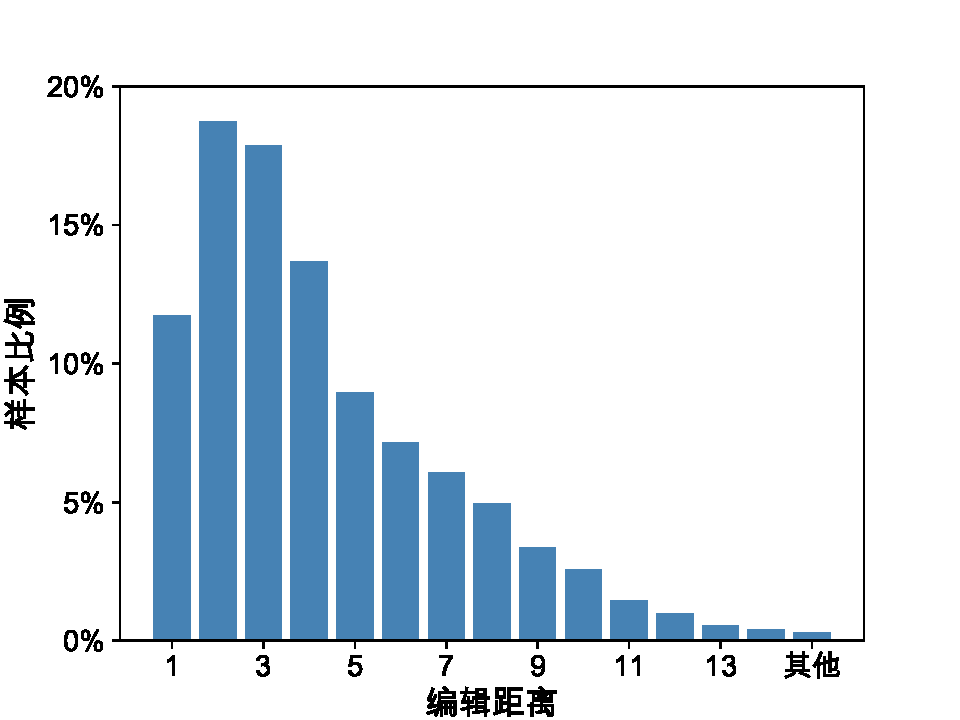
\includegraphics[scale=0.5]{figure/fig4-1.pdf}
    \caption{LCQMC$_{DDA}$数据编辑距离统计}
    \label{fig4-1}
\end{figure}

\subsection{标签修正策略分析}\label{4.3.3 标签修正策略分析}

本节使用上述三个基线判别模型集成投票的方式修正样本的定向诱导标签。
若多票($>=2$)与定向标签一致,则保留定向标签为样本最终标签;
否则,将预测结果为复述关系的概率均值$p$作为标签判断依据。
若$p>=\alpha$,则将定向标签为0的样本修正为标签为1的正样本;
若$p<=\beta$,则将定向标签为1的样本修正为标签为0的负样本。
借助LCQMC$_{DDA}$人工标注的测试集可统计出标签修正的准确度,
表~\ref{table4-6}~和表~\ref{table4-7}~分别展示了$\alpha$和$\beta$取值对正负样本修正准确度的影响。
其中,“修正”表示修正后的标签与人工评估标签一致;
“误修正”表示修正后的标签与人工评估标签不一致;“净修正”是两者差值。

\begin{table}
    \caption{正样本标签阈值统计表}
    \centering
    \newcommand{\tabincell}[2]{\begin{tabular}{@{}#1@{}}#2\end{tabular}}
    \begin{tabular}{l|c|c|c}
    \toprule[0.7pt]
    \textbf{$\alpha$\qquad\enspace  } &  \enspace\textbf{修正}  \enspace&  \;\textbf{误修正} \; & \enspace \textbf{净修正} \\
    \midrule[0.7pt]

    0.95 & 144 & 12 & \enspace 132\\
    \textbf{0.92} & \textbf{161} & \textbf{17} & \enspace \textbf{144}\\
    0.8 & 173 &  41 & \enspace 132\\
    0.7 & 182 &  51 & \enspace 131\\
    0.6 & 188 &  59 & \enspace 129\\
    0.5 & 192 &  71 & \enspace 121\\

    \bottomrule[0.7pt]
    \end{tabular}
    \label{table4-6}
\end{table}

由表可见,当$\alpha=0.92$时,将负样本修正为正样本的净修正量最多;
当$\beta=0.5$时,将正样本修正为负样本的净修正量最多。
由于DDA策略构造的负样本具有一定的迷惑性,所以模型预测负样本为复述关系的概率整体偏高,即$\beta$的取值偏高。
最终,本章使用该阈值对16.3万条训练样本进行标签修正,共将31,596条样本修正为正样本,9,140条样本修正为负样本。
本章对标签修正前后的训练数据进行了数据增强对比实验,在BERT$_{base}$基线上的结果如表~\ref{table4-3}~所示,标签修正后的数据(+DDA)比未修正的数据(+DDA$_{noise}$)在增强训练后的准确率平均提升约5.8\%。

\begin{table}
    \caption{负样本标签阈值统计表}
    \centering
    \newcommand{\tabincell}[2]{\begin{tabular}{@{}#1@{}}#2\end{tabular}}
    \begin{tabular}{l|c|c|c}
    \toprule[0.7pt]
    \textbf{$\beta$\qquad\enspace } &   \enspace \textbf{修正}  \enspace& \; \textbf{误修正} \;&  \enspace \textbf{净修正} \\
    \midrule[0.7pt]

    0.1 & 37 & 0 & \enspace 37 \\
    0.2 & 49 & 1 & \enspace 48 \\
    0.3 & 60 & 2 & \enspace 58 \\
    0.4 & 72 & 4 & \enspace 68 \\
    \textbf{0.5} & \textbf{78} & \textbf{5} & \enspace \textbf{73} \\

    \bottomrule[0.7pt]
    \end{tabular}
    \label{table4-7}
\end{table}

\subsection{训练集规模实验分析}

模型在较小的数据集上进行训练时,过拟合现象往往更为严重。
为了探究DDA对于不同规模数据的增强效果,本章将LCQMC的数据分割为不同大小的子集,
其数据量分别为:$\{4w,\ 8w,\ 12w,\ 16w,20w,ALL\}$(ALL表示LCQMC全部数据)。
本章在不同规模的子集上对BERT$_{base}$进行DDA数据增强实验,并在LCQMC测试集上评估其准确率。

\begin{figure}[h]
    \centering
      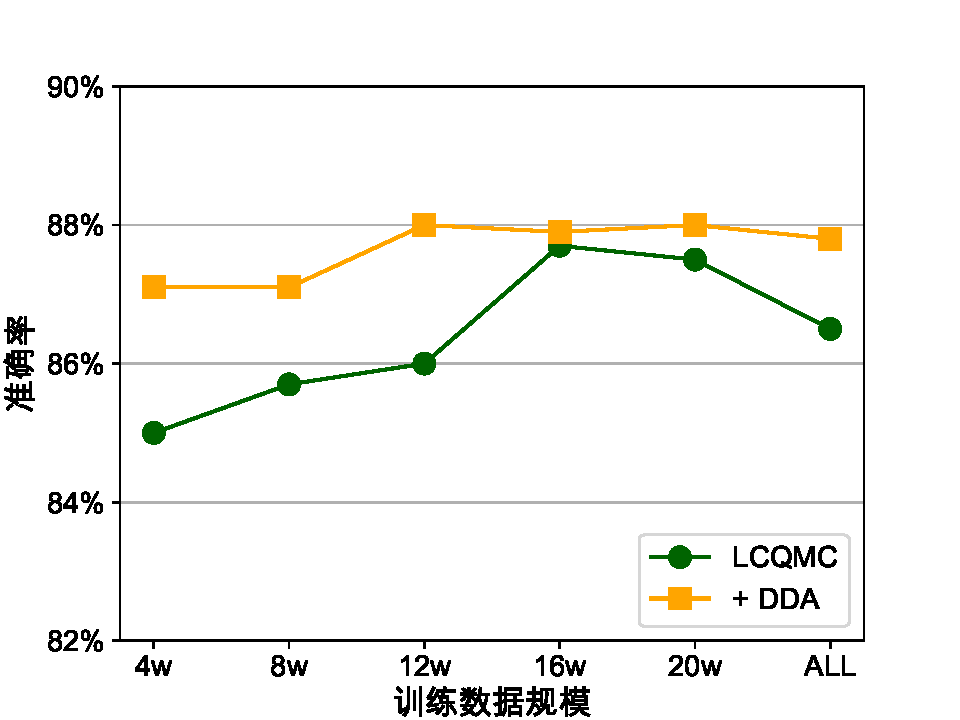
\includegraphics[scale=0.5]{figure/fig4-2.pdf}
    \caption{LCQMC测试集性能曲线}
    \label{fig4-2}
\end{figure}

如图~\ref{fig4-2}~所示,当训练数据量较小时,DDA策略与基线的差异更加明显,这表明DDA对规模较小的数据集效果更为显著。
此外,从图中可以明显看出,当LCQMC的数据量增大到16万后,基线模型逐渐出现过拟合现象,继续增加数据量性能反而有下降趋势。
反观DDA数据增强策略,其性能曲线并未随着数据量的增加有明显下降趋势。
DDA增强数据中包含一些难度较大、具有迷惑性的样本,能够有效提高神经网络模型的泛化能力和鲁棒性,抑制过拟合现象的产生。

\subsection{显著性分析}

本章使用显著性检验确保实验结果并非偶然结果,即重复进行了多次实验(5次)计算使用DDA数据增强策略前后,基线在各个测试集上准确率指标的P-value值。
由表~\ref{table4-8}~可见,本章所提出的DDA数据增强方法在多个基线上的不同测试集结果P-value值均小于0.05,即均存在显著提升。

\begin{table}[h]
    \caption{显著性分析结果}
    \centering
    \newcommand{\tabincell}[2]{\begin{tabular}{@{}#1@{}}#2\end{tabular}}
    \begin{tabular}{l|c|c|c}
    \toprule[0.7pt]
    \textbf{模型} & \enspace\textbf{LCQMC}\enspace & \enspace\textbf{LCQMC$_{DDA}$}\enspace & \enspace\textbf{CQM$_{robust}$} \\
    \midrule[0.7pt]

    BERT$_{base}$   & 3.4e-3 & 8.7e-4 & \enspace 5.2e-4 \\
    RoBERTa$_{large}$ & 4.2e-2 & 1.3e-3 & \enspace 4.1e-3 \\
    MacBERT$_{large}$\quad\quad & 1.3e-3 & 1.9e-2 & \enspace 3.2e-3 \\

    \bottomrule[0.7pt]
    \end{tabular}
    \label{table4-8}
\end{table}

\section{本章小结}

本章提出了一种面向问题复述识别任务的定向数据增强策略DDA,该方法可以定向构造蕴含精细语义的高质量样本,促进训练数据的自动扩展。
实验结果表明DDA能够有效提高问题复述识别模型的鲁棒性与泛化能力。
然而,本章并未对模型性能提升的细节展开进一步的实验分析与探究,从而无法精确衡量模型优化前后的能力差异。
% 然而,本章对于模型鲁棒性提升的细节尚未展开进一步的探究。
因此,下一章将基于中文语法特征对问题复述识别模型进行系统化的评估,深入分析模型具体能力及其鲁棒性的变化。
% 在未来的工作中,我们将进一步提高定向生成环节的样本质量,以及对标签修正环节进行优化。
% 同时,尝试将该方法应用到其他NLP领域中。
\chapter{面向问题复述识别的模型综合能力鲁棒性研究}\label{5.point3}

上一章采用定向数据增强方法扩充了大量高质量、多元化的训练样本,强化了问题复述识别模型的精细语义感知能力,一定程度上提高了模型的鲁棒性。
鲁棒性能够反映出模型的实用能力,尤其在语法灵活、语义多样的中文领域,对模型鲁棒性的研究尤为重要。
然而,上一章的实验仅得出模型鲁棒性有所提升的简单结论,缺少对其鲁棒性变化的详细分析与探讨。
为此,本章构造了一个符合中文语言学特征的评估数据集CQM$_{robust}$,用以系统化评估问题复述识别模型的能力及鲁棒性。
CQM$_{robust}$包含3种语言特征、13个测试子类,共计32个测试项,且其所有数据均来源于搜索引擎中的真实提问。
大量的实验表明,CQM$_{robust}$比传统数据集难度更大,更具有挑战性,
且能够按不同语言现象对模型进行详细评估,有助于诊断现有模型的优势和劣势。
下面将详细介绍本章的研究动机、数据构造方案以及实验分析。

\section{引言}

在过去的几年里,预训练语言模型在NLP领域引起了轰动,其在许多传统的数据集上取得了优异的性能,
包括问题复述数据集Quora\cite{iyer2017first}、LCQMC\cite{liu2018lcqmc}、BQ\cite{chen2018bq}和AFQMC\footnote{蚂蚁技术探索会议(ATEC)开发者竞赛}。
然而,与其性能表现不一致的是,目前最先进的模型在现实世界的场景中仍会出现令人惊讶的错误。
如表~\ref{table5-1}~所示( {\kai\colorbox{lightgreen}{\color{darkgreen}绿色}} 和 {\kai\colorbox{lightred}{\color{darkred}红色}} 部分标记出问题之间的细微差别),
第一个例子中,RoBERTa模型无法区分两个问题中{\kai“蔬菜”}和{\kai“绿色蔬菜”}之间的细微差异,从而将这两个问题误判为语义等价的复述关系;
第三个例子中,模型没有判断出{\kai“监狱”}与{\kai“牢房”}两个词为同义,从而将其误判为非复述关系。
由此可见,现有模型不能以灵活方式处理简单的案例。

% 表: 例子
\begin{table}
    \caption{CQM$_{robust}$数据样例}
    % \begin{spacing}{1.1}
    % \small
    \centering
    \newcommand{\tabincell}[2]{\begin{tabular}{@{}#1@{}}#2\end{tabular}}
    \begin{tabular}{llcc}
    \toprule[0.7pt]
     \textbf{问题1} & \textbf{问题2} & \textbf{标签} & \textbf{RoBERTa} \\
    \midrule[0.7pt]
    婴儿吃什么蔬菜好? & 婴儿吃什么\colorbox{lightgreen}{\color{darkgreen}绿色}蔬菜好?\;\  & 0 & 1 \\\hline
    心率过\colorbox{lightred}{\color{darkred}慢}有什么危害 & 心率过\colorbox{lightgreen}{\color{darkgreen}快}有什么危害 & 0 & 1 \\\hline
    求关于\colorbox{lightred}{\color{darkred}监狱}的电视剧\quad\ & 求关于\colorbox{lightgreen}{\color{darkgreen}牢房}的电视剧 & 1 & 0 \\
    
        
    \bottomrule[0.7pt]
    
    \end{tabular}
    \label{table5-1}
    % \end{spacing}
\end{table}

近期,关于神经网络模型鲁棒能力的研究吸引了大量学者的关注。
早期的研究工作通过创建某种类型的对抗性样本,并以此评估神经模型的鲁棒性\cite{jia2017adversarial,alzantot2018generating,ren2019generating,jin2020bert}。
如表~\ref{table5-1}~中的样例,对抗性样本指的是在原始样本中加入一些不影响人类识别但却容易愚弄模型的扰动。
也有一些研究通过人机对抗的方式构造对抗性样本,
如Nie等利用人类与模型在多轮循环对抗中构建的对抗性自然语言推理数据集(Natural Language Inference,简称NLI)\cite{nie2019adversarial},
其在多轮对抗中数据集难度逐渐上升,对NLI模型的能力提出新的挑战。
此外,相关研究开始尝试借助对抗训练的方案\cite{min2020syntactic,bao2021defending,wang2021natural}抵御对抗性样本的攻击。
这些努力更加有利于发现和解决模型鲁棒性缺陷。

然而,以往关于模型鲁棒性的研究仅针对某中特定场景下的数据,或是只使用了少量的数据变化方法,缺乏综合性的评估方案。
合理的评估方案应当以多样化的数据综合评估模型的表现,而不是单一的攻击模型某种能力漏洞。
为了更全面地评估模型的性能,Ribeiro等提出了一种用于NLP模型行为测试的方法和配套工具CHECKLIST\cite{ribeiro2020beyond}。
用户可以借助其定制测试列表,从多个抽象概念中生成测试样本。
复旦大学发布的模型鲁棒性评测平台TextFlint\cite{gui2021textflint}也为模型鲁棒性评测提供了一站式解决方案。
然而,CHECKLIST和TextFlint以模板化方式大量生产的样本不能客观地代表真实世界的自然语言,
且缺乏针对特定语言和特定任务的语法现象分析。

为此,本章创建了一个开放领域的中文数据集CQM$_{robust}$,用于评估问题复述识别模型的综合能力及鲁棒性。
如表~\ref{table5-2}~所示,CQM$_{robust}$包含3大类语言特征、13个测试子类,共计32个测试项。
并且CQM$_{robust}$中的所有问题均源于百度商业搜索引擎\footnote{http://www.baidu.com/}中的用户真实提问,
而非刻意通过人工撰写的非自然问句,
这有利于客观评价模型的实际应用能力。
本章的主要贡献有:

\begin{enumerate}
    \item 
    构建了一个系统化的中文问题复述识别评估基准CQM$_{robust}$,其中所有问题均为百度搜索引擎真实数据。
    \item 
    CQM$_{robust}$比传统数据集更加具有挑战性,并且能够按语言现象诊断模型,区分不同模型的优势和劣势。
\end{enumerate}

本章的组织形式如下:第1节为引言部分;第2节详细介绍CQM$_{robust}$数据集的结构体系;第3节介绍了数据集的构造方案;第4节介绍实验部分并进行结果分析;第5节对本章内容进行总结。


\section{CQM$_{robust}$体系结构}

CQM$_{robust}$旨在按照中文语言现象对模型进行详细评估,这些语言现象对评价模型的能力至关重要。
因此,本章将测试数据归纳为3种符合语言学特征的类别,包括词法特征(Lexical Features)、
句法特征(Syntactic Features)和语境特征(Pragmatic Features)。
如表~\ref{table5-2}~所示,本节将介绍CQM$_{robust}$各个能力类别的详细特点。

\subsection{词法特征}\label{5.2.1 词法特征}

词法特征考察模型对各类词汇理解程度。
词是独立但有意义的最小语义单元,一个词的变化也会改变整个句子的意义。
本章将词法特征归纳为如下6个子类别:

% 表: CQM\textsubscript{robust}数据集统计
\begin{table}[!h]
    \caption{CQM\textsubscript{robust}评估体系及基线模型评估结果}
    % \tiny
    \centering
    \newcommand{\tabincell}[2]{\begin{tabular}{@{}#1@{}}#2\end{tabular}}
    \resizebox{155mm}{108mm}
    {
    \small
    %\begin{adjustbox}{max width=\textwidth}
    \begin{tabular}{c|c|c|c|cccccc|l}
    \toprule[0.7pt]
    %  \textbf{ \tabincell{c}{Coarse-grained\\ Categories}} & \textbf{\tabincell{c}{Fine-grained\\ Categories}} & \textbf{\tabincell{c}{Perturbation\\ Operations}} & \textbf{Examples and Translation} & \textbf{Label} & \textbf{\#Y / \#N} \\
      \textbf{ \tabincell{c}{类别}} & \textbf{\tabincell{c}{子类}} & \textbf{\tabincell{c}{扰动\\操作}} & {\tabincell{c}{\textbf{标签} \\ \#1 / \#0}} &{ \tabincell{c}{BERT\\base}}&{ \tabincell{c}{ERNIE\\base}} & { \tabincell{c}{RoBERTa\\base}}&{ \tabincell{c}{MacBERT\\base}}&{ \tabincell{c}{RoBERTa\\large}}&{ \tabincell{c}{MacBERT\\large}}& \tabincell{c}{样例及翻译} \\
    \midrule[0.7pt]
    
    % Lexical
    
    % basic
    \multirow{55}*{{\rotatebox{90}{\textbf{词法}}}} & \multirow{22}*{\tabincell{c}{基础\\词汇}} & 插入名词 &
     -/539
    &
    41.4±3.4 & 40.8±2.1 & \underline{43.0±0.7} & 41.4±2.5 & \textbf{45.4±4.1} & 37.3±2.4 &
     \tabincell{l}{\textbf{E1}: \label{example:E1}鸡蛋怎么炒好吃\;/\; 鸡蛋\colorbox{lightgreen}{\color{darkgreen}面}怎么炒好吃 \\
    \quad\;\;\, how to fry eggs\;/\; how to fry egg 
     \colorbox{lightgreen}{\color{darkgreen}noodles}}
     \\\cline{3-11}
    
     & & 插入动词& 
     -/131
     &
     \underline{39.4±0.4} & 33.8±2.6 & 37.4±2.0 & 35.9±2.7 & \textbf{39.9±3.1} & 29.5±3.8 &
     \tabincell{l}{\specialrule{0em}{0em}{1mm}\textbf{E2}: \label{example:E2}伤口用什么好\;/\; 伤口用什么\colorbox{lightgreen}{\color{darkgreen}消毒}好\\
    \quad\;\;\,what is good for the wound\;/\; how to \colorbox{lightgreen}{\color{darkgreen}disinfect} the wound
    }
    \\\cline{3-11}
    
     & & 插入形容词 & 
     -/458
     &
     23.5±1.9 & 19.2±3.7 & \textbf{26.9±4.4} & \underline{23.9±4.2} & 18.1±2.4 & 10.4±2.1 &
     \tabincell{l}{\specialrule{0em}{0em}{1mm}\textbf{E3}: \label{example:E3}有哪些类型的app\;/\; 有哪些类型的\colorbox{lightgreen}{\color{darkgreen}移动}app\\
     \quad\;\;\,what are types of apps\;/\; what are types of \colorbox{lightgreen}{\color{darkgreen}mobile} apps
    }
    \\\cline{3-11}
    
     & & 插入副词& 
      -/302
     &
     3.7±0.5 & 4.2±0.5 & 3.8±0.6 & \underline{4.4±1.2} & \textbf{5.8±1.5} & 3.1±1.1 &
     \tabincell{l}{\specialrule{0em}{0em}{1mm}\textbf{E4}: \label{example:E4}为什么打嗝\;/\; 为什么\colorbox{lightgreen}{\color{darkgreen}老}打嗝\\
     \quad\;\;\,why burp\;/\; why \colorbox{lightgreen}{\color{darkgreen}always} burp
    }
    \\\cline{3-11}
    
    %/v./adj./adv. 
     & & 替换名词 & 
      -/702
     &
     86.6±0.3 & 86.7±0.1 & 88.3±0.3 & \underline{88.8±1.2} & \textbf{89.4±1.6} &  87.8±0.7&
     \tabincell{l}{\specialrule{0em}{0em}{1mm}\textbf{E5}: \label{example:E5}申请美国\colorbox{lightred}{\color{darkred}绿卡}流程\;/\; 申请美国\colorbox{lightgreen}{\color{darkgreen}签证}流程\\
    \quad\;\;\,U.S. \colorbox{lightred}{\color{darkred}green card} application process\;/\; U.S.  \colorbox{lightgreen}{\color{darkgreen}visa} application process
    }
    \\\cline{3-11}
    
     & & 替换动词& 
      -/466
     &
     71.7±1.1 &77.6±0.8 & 76.9±0.4 & 76.5±1.2 & \underline{81.0±1.6} & \textbf{81.5±2.2} &
     \tabincell{l}{\specialrule{0em}{0em}{1mm}\textbf{E6}: \label{example:E6}为什么\colorbox{lightred}{\color{darkred}下蹲}膝盖疼\;/\; 为什么\colorbox{lightgreen}{\color{darkgreen}下跪}膝盖疼\\
     \quad\;\;\,why knee pain when \colorbox{lightred}{\color{darkred}squatting}\;/\; why knee pain when \colorbox{lightgreen}{\color{darkgreen}kneeling}
    }
    \\\cline{3-11}
    
     & & 替换形容词 & 
      -/472
     &
     74.3±2.1 & 80.0±1.0 & 77.6±0.7 & 81.6±0.5 & \textbf{82.7±1.1} & \underline{82.7±1.6} &
     \tabincell{l}{\specialrule{0em}{0em}{1mm}\textbf{E7}: \label{example:E7}耳朵出血\colorbox{lightred}{\color{darkred}严重}吗\;/\; 耳朵出血\colorbox{lightgreen}{\color{darkgreen}正常}吗\\
     \quad\;\;\,is the ear bleeding \colorbox{lightred}{\color{darkred}serious}\;/\; is the ear bleeding \colorbox{lightgreen}{\color{darkgreen}normal}
    }
    \\\cline{3-11}
    
    & & 替换副词& 
     -/188
    &
    19.1±6.1 & 19.3±4.4 & 16.3±3.8 & 23.9±4.6 & \textbf{59.0±4.0} & \underline{56.2±2.0} &
     \tabincell{l}{\specialrule{0em}{0em}{1mm}\textbf{E8}: \label{example:E8}为什么会\colorbox{lightred}{\color{darkred}经常}头晕\;/\; 为什么会\colorbox{lightgreen}{\color{darkgreen}有点}头晕\\
     \quad\;\;\,why \colorbox{lightred}{\color{darkred}regularly} feel dizzy\;/\; why  \colorbox{lightgreen}{\color{darkgreen}slightly} feel dizzy
    }
    \\\cline{3-11}
    
     & & 替换数词&  
      -/1116
     &
     83.2±1.4 & \underline{91.4±0.4} & 85.9±1.8 & 87.2±0.9 & 88.1±0.5 & \textbf{91.9±1.1} &
     \tabincell{l}{\specialrule{0em}{0em}{1mm}\textbf{E9}: \label{example:E9}血压\colorbox{lightred}{\color{darkred}130}/100高吗\;/\;
     血压\colorbox{lightgreen}{\color{darkgreen}120}/100高吗\\
     \quad\;\;\,is blood pressure \colorbox{lightred}{\color{darkred}130}/100 high \;/\; is blood pressure \colorbox{lightgreen}{\color{darkgreen}120}/100 high}
    \\\cline{3-11}
    
     & & 替换量词&  
      -/22
     &
     {30.3±6.9} & 25.7±5.2 & 33.3±2.6 & \textbf{34.9±2.6} & 27.3±0.0 & \underline{34.8±10.5} &
     \tabincell{l}{\specialrule{0em}{0em}{1mm}\textbf{E10}: \label{example:E10}一\colorbox{lightred}{\color{darkred}束}花多少钱\;/\;
     一\colorbox{lightgreen}{\color{darkgreen}枝}花多少钱\\
     \qquad\, how much is \colorbox{lightred}{\color{darkred}a bunch of} flower \;/\; how much is  \colorbox{lightgreen}{\color{darkgreen}a}flower}
    \\\cline{3-11}
    
     & & 替换词组 &   
      -/197
     &
     \underline{98.0±0.0} & \textbf{98.1±0.2} & 96.6±0.3 & 97.8±0.5 & 97.8±0.2 & 97.5±0 &
     \tabincell{l}{\specialrule{0em}{0em}{1mm}\textbf{E11}: \label{example:E11}如何\colorbox{lightred}{\color{darkred}提高自己的记忆力}\;/\; 如何\colorbox{lightgreen}{\color{darkgreen}增加自己的实力}\\
     \qquad\, how to \colorbox{lightred}{\color{darkred}improve my memory}\;/\; how to \colorbox{lightgreen}{\color{darkgreen}increase my strength}
     }
    
    \\\cline{2-11}
    
    % ner
     & \multirow{8}*{\tabincell{c}{命名\\实体}} & 替换地点 & 
      -/458
     &
     \textbf{96.0±0.6} & \underline{95.7±0.2} & 95.4±0.4 & 95.0±0.4 & 94.7±0.4&94.5±0.5 &
     \tabincell{l}{\specialrule{0em}{0em}{1mm}\textbf{E12}: \label{example:E12}\colorbox{lightred}{\color{darkred}山西}春节习俗 \;/\;\colorbox{lightgreen}{\color{darkgreen}陕西}春节习俗 \\
     \qquad\, \colorbox{lightred}{\color{darkred}Shanxi} spring festival customs\;/\; \colorbox{lightgreen}{\color{darkgreen}Shannxi} spring festival customs}
    \\\cline{3-11}
    
     &  & 替换机构 &  
      -/264
     &
     \textbf{94.9±0.2} & \underline{94.3±0.6} & 91.2±1.4 & 93.4±0.7 & 93.5±0.3 & 93.8±0.1 &
      \tabincell{l}{\specialrule{0em}{0em}{1mm}
      \textbf{E13}: \label{example:E13}\colorbox{lightred}{\color{darkred}北京邮电大学}附近酒店 \;/\; \colorbox{lightgreen}{\color{darkgreen}南京邮电大学}附近酒店\\
     \qquad\, hotels near \colorbox{lightred}{\color{darkred}BUPT}\;/\; hotels near \colorbox{lightgreen}{\color{darkgreen}NJUPT}}
    \\\cline{3-11}
     
     &  & 替换人物 &  
      -/468
     &
     90.3±1.3 & 91.0±0.9  & 88.7±1.6 & 91.4±1.6 & \underline{92.3±1.3}& \textbf{93.2±1.1} &
      \tabincell{l}{\specialrule{0em}{0em}{1mm}
      \textbf{E14}: \label{example:E14}\colorbox{lightred}{\color{darkred}陈龙}的妻子 \;/\; \colorbox{lightgreen}{\color{darkgreen}成龙}的妻子\\
     \qquad\, wife of \colorbox{lightred}{\color{darkred}Long Chen}\;/\; wife of \colorbox{lightgreen}{\color{darkgreen}Jackie Chan}}
    \\\cline{3-11}
     
     &  & 替换物品 &  
      -/170
     &
     83.7±2.6 &\underline{88.2±2.1} & 82.4±6.9 & 83.3±0.3 & 86.0±1.7 & \textbf{88.8±4.4} &
      \tabincell{l}{\specialrule{0em}{0em}{1mm}
      \textbf{E15}: \label{example:E15}\colorbox{lightred}{\color{darkred}iphone 6}多少钱 \;/\; \colorbox{lightgreen}{\color{darkgreen}iphone6x}多少钱\\
     \qquad\, how much is \colorbox{lightred}{\color{darkred}iphone 6}\;/\; how much is \colorbox{lightgreen}{\color{darkgreen}iphone6x}}
    \\\cline{2-11}
     
    % synonym
     & \multirow{8}*{同义词} & 替换名词 &  
      405/-
     &
     51.1±1.1 & 59.7±1.3 & 59.7±2.2 & 60.7±2.0 & \underline{63.3±3.1} &\textbf{71.6±4.0} & 
     \tabincell{l}{\specialrule{0em}{0em}{1mm}
     \textbf{E16}: \label{example:E16}\colorbox{lightred}{\color{darkred}猕猴桃}的功效 \;/\;
      \colorbox{lightgreen}{\color{darkgreen}奇异果}的功效\\
    \qquad\, health benefits of \colorbox{lightred}{\color{darkred}Chinese gooseberry}\;/\;
    health benefits of \colorbox{lightgreen}{\color{darkgreen}Kiwi}}
    \\\cline{3-11}
    
     &  & 替换动词 &  
      372/-
     &
     80.0±0.9& 81.1±1.6 & 82.5±0.0 & 83.2±1.2 & \underline{84.0±2.0} & \textbf{88.1±1.4} &
      \tabincell{l}{\specialrule{0em}{0em}{1mm}
      \textbf{E17}: \label{example:E17}什么果汁可以\colorbox{lightred}{\color{darkred}减肥} \;/\; 什么果汁可以\colorbox{lightgreen}{\color{darkgreen}减重}\\
     \qquad\, what juice can \colorbox{lightred}{\color{darkred}lose weight}\;/\; what juice can \colorbox{lightgreen}{\color{darkgreen}slim}}
    \\\cline{3-11}
     
     &  & 替换形容词 &  
      453/-
     &
     75.7±1.3 & 77.3±1.1 & 78.8±2.5 & 74.8±0.5 & \underline{79.4±3.4} & \textbf{88.5±1.3} &
      \tabincell{l}{\specialrule{0em}{0em}{1mm}
      \textbf{E18}: \label{example:E18}\colorbox{lightred}{\color{darkred}有趣}搞笑的广告词 \;/\; \colorbox{lightgreen}{\color{darkgreen}幽默}搞笑的广告词\\
     \qquad\, \colorbox{lightred}{\color{darkred}funny} advertising words\;/\; \colorbox{lightgreen}{\color{darkgreen}humerous} advertising words}
    \\\cline{3-11}
     
     &  & 替换副词 &  
      26/-
     &
     \underline{98.7±2.1} & \textbf{100.0±0.0} & \textbf{100.0±0.0} & \textbf{100.0±0.0} &\textbf{100±0.0} &\textbf{100.0±0.0} & 
      \tabincell{l}{\specialrule{0em}{0em}{1mm}
      \textbf{E19}: \label{example:E19}\colorbox{lightred}{\color{darkred}总是}想睡觉是为什么 \;/\; \colorbox{lightgreen}{\color{darkgreen}老是}想睡觉是为什么\\
     \qquad\, why \colorbox{lightred}{\color{darkred}always} want to sleep \;/\; why \colorbox{lightgreen}{\color{darkgreen}repeatedly} want to sleep}
    \\\cline{2-11}
    
    % Antonym
     & 反义词 & 替换形容词 & 
      -/305
     &
     50.6±3.4 &69.6±2.9 & 65.0±1.5 & 73.1±4.3 &\textbf{91.7±2.3} &\underline{90.7±2.3} & 
      \tabincell{l}{\specialrule{0em}{0em}{1mm}
      \textbf{E20}: \label{example:E20}什么水果脂肪\colorbox{lightred}{\color{darkred}低} \;/\; 
      什么水果脂肪\colorbox{lightgreen}{\color{darkgreen}高}\\
      \qquad\, what fruit is  \colorbox{lightred}{\color{darkred}low} in fat\;/\;
      what fruit is \colorbox{lightgreen}{\color{darkgreen}high} in fat
      }
      
    \\\cline{2-11}
    % negation
    
     & \multirow{6}*{否定} & 否定动词 &  
      -/153
     &
     69.9±9.6 & 88.9±1.3 & 84.8±2.9 & \textbf{93.3±1.3} & 88.4±0.9 & \underline{91.4±3.4} & 
     \tabincell{l}{\specialrule{0em}{0em}{1mm}
     \textbf{E21}: \label{example:E21}为什么宝宝哭\;/\; 为什么宝宝\colorbox{lightgreen}{\color{darkgreen}不}哭 \\
     \qquad\, why baby cries\;/\; why baby \colorbox{lightgreen}{\color{darkgreen}doesn't} cry
     }
    \\\cline{3-11}
     &  & 否定形容词 &  
      -/139
     &
     73.1±8.5 & 84.2±1.2 & 82.7±1.4 & \underline{88.0±1.5} & 88.0±2.9 & \textbf{89.4±1.0} & 
      \tabincell{l}{\specialrule{0em}{0em}{1mm}
    \textbf{E22}: \label{example:E22}为什么苹果是红的\;/\; 为什么苹果\colorbox{lightgreen}{\color{darkgreen}不是}红的 \\
     \qquad\, why apple is red\;/\; why apple is \colorbox{lightgreen}{\color{darkgreen}not} red }
    \\\cline{3-11}
     
     &  & 否定反义词 & 
      59/-
     &
     29.9±2.5 & 34.4±2.5 & 39.0±1.7 & 31.1±2.5 & \underline{40.7±1.7} & \textbf{53.6±0.9} & 
     \tabincell{l}{\specialrule{0em}{0em}{1mm}
     \textbf{E23}: \label{example:E23}\colorbox{lightred}{\color{darkred}激动}怎么办\;/\; \colorbox{lightgreen}{\color{darkgreen}无法}\colorbox{lightgreen}{\color{darkgreen}平静}怎么办 \\
    \qquad\, what to do if too \colorbox{lightred}{\color{darkred}excited}\;/\; what to do if \colorbox{lightgreen}{\color{darkgreen}can't}\colorbox{lightgreen}{\color{darkgreen}calm down}
     }
     
    \\\cline{2-11}
    
    % tense
     & \multirow{4}*{{\tabincell{c}{时态}}} & 插入时间词 & 
      -/120
     &
     26.6±2.1 & 29.1±2.1 & 33.1±0.9 & \underline{41.7±3.3} & \textbf{47.5±5.4} & 33.6±8.5  &
     \tabincell{l}{\specialrule{0em}{0em}{1mm}
     \textbf{E24}: \label{example:E24}北京会下雨吗\;/\; 北京\colorbox{lightgreen}{\color{darkgreen}明天}会下雨吗 \\
     \qquad\, will it rain in Beijing\;/\; will it rain in Beijing\colorbox{lightgreen}{\color{darkgreen}tomorrow}
     }
     \\\cline{3-11}
     & & 替换时间词 & 
      -/114
     &
     44.1±6.1 & 67.8±2.6 & 55.0±0.5 & 53.8±1.3 & \underline{70.4±6.1} & \textbf{78.6±5.8} &
     \tabincell{l}{\specialrule{0em}{0em}{1mm}
    \textbf{E25}: \label{example:E25}\colorbox{lightred}{\color{darkred}昨天}下雪\colorbox{lightred}{\color{darkred}了}吗\;/\; \colorbox{lightgreen}{\color{darkgreen}明儿}会下雪吗 \\
    \qquad\, was it \colorbox{lightred}{\color{darkred}snow} yesterday\;/\; will it \colorbox{lightgreen}{\color{darkgreen}snow} tomorrow
     }
    %  \\\cline{2-11}
    % \specialrule{0em}{0em}{2mm}
    %  &\multicolumn{2}{c|}{\textbf{Micro / Macro Acc}}&67.2 / 61.4 & 71.0 / 65.5  & \underline{74.1} / \underline{70.2}  & \textbf{74.4} / \textbf{70.7} & \tabincell{l}{-}
    
     \\\midrule[0.7pt]
     
    % Syntactic
    \multirow{8}*{{\rotatebox{90}{\textbf{句法}}}}
     & 对称角色 & 交换 & 
      533/-
     &
     \underline{97.3±0.4} & \textbf{98.0±0.1} & 95.2±1.7 & 95.9±0.7 & 93.3±0.9 & 92.5±1.9  &
     \tabincell{l}{\textbf{E26}: \label{example:E26}\colorbox{lightred}{
    \color{darkred}鱼}和\colorbox{lightred}{\color{darkred}鸡蛋}能一起吃吗\;/\; 
      \colorbox{lightgreen}{\color{darkgreen}鸡蛋}和\colorbox{lightgreen}{\color{darkgreen}鱼}能一起吃吗\\
      \qquad\, can I eat \colorbox{lightred}{\color{darkred}fish} with \colorbox{lightred}{\color{darkred}egg}\;/\; can I eat \colorbox{lightgreen}{\color{darkgreen}egg} with \colorbox{lightgreen}{\color{darkgreen}fish}
    }
    \\\cline{2-11}
     
      & 非对称角色 & 交换 & 
       -/497
      &
      14.5±2.0 & 18.3±3.7 & 26.8±3.2 & 26.4±2.5 & \textbf{52.0±4.6} & \underline{49.1±10.8} &
      \tabincell{l}{\specialrule{0em}{0em}{1mm}
      \textbf{E27}: \label{example:E27}\colorbox{lightred}{\color{darkred}北京}到\colorbox{lightred}{\color{darkred}上海}航班\;/\; 
      \colorbox{lightgreen}{\color{darkgreen}上海}到\colorbox{lightgreen}{\color{darkgreen}北京}航班\\
      \qquad\, \colorbox{lightred}{\color{darkred}Beijing} to \colorbox{lightred}{\color{darkred}Shanghai} flights\;/\;
      \colorbox{lightgreen}{\color{darkgreen}Shanghai} to \colorbox{lightgreen}{\color{darkgreen}Beijing} flights
    }
    \\\cline{2-11}
    & \tabincell{c}{反义非对称} & 交换+反义 &
     49/-
     &
      \textbf{47.6±3.4}& 37.4±7.7 & \underline{44.2±1.1} & 25.8±3.1 & 23.1±6.7 & 29.9±1.9 &
     \tabincell{l}{\specialrule{0em}{0em}{1mm}
      \textbf{E28}: \label{example:E28}\colorbox{lightred}{\color{darkred}男人}比\colorbox{lightred}{\color{darkred}女人}更\colorbox{lightred}{\color{darkred}高}吗\;/\; 
      \colorbox{lightgreen}{\color{darkgreen}女人}比\colorbox{lightgreen}{\color{darkgreen}男人}更\colorbox{lightgreen}{\color{darkgreen}矮}吗\\
      \qquad\, are \colorbox{lightred}{\color{darkred}men}\colorbox{lightred}{\color{darkred}taller}  than \colorbox{lightred}{\color{darkred}women}\;/\; are \colorbox{lightgreen}{\color{darkgreen}women}\colorbox{lightgreen}{\color{darkgreen}shorter} than \colorbox{lightgreen}{\color{darkgreen}men}
    }
    \\\cline{2-11}
     
     & 主被动 & 插入/交换 &
      94/37
     &
     76.8±1.4& 72.5±0.0 & \underline{77.4±0.9} & 74.0±0.7 & \textbf{85.2±1.4} & 74.8±2.2 &
     \tabincell{l}{
     \specialrule{0em}{0em}{1mm}
      \textbf{E29}: \label{example:E29}梦见狗咬左腿\;/\;梦见\colorbox{lightgreen}{\color{darkgreen}被}狗咬左腿\\
     \qquad\, dreamed of being bitten by a dog\;/\; 
     dreamed of being bitten by a dog
     } 
    %  & Voice & insert passive word &
    %   94/37
    %  &
    %  \underline{76.8±1.4}& 72.5±0.0 & \textbf{85.2±1.4} & 74.8±2.2 &
    %  \tabincell{l}{
    %  \specialrule{0em}{0em}{1mm}
    %   \textbf{E29}: \label{example:E29}狗咬了猫怎么办\;/\;猫\colorbox{lightgreen}{\color{darkgreen}被}被狗咬了怎么办\\
    %  \qquad\, what to do if dog bites cat\;/\; 
    %  what to do if cat \colorbox{lightgreen}{\color{darkgreen}is bitten} by dog
    %  } 
    %  \\\cline{2-11}
    %  \specialrule{0em}{0em}{1mm}
    %  &\multicolumn{2}{c|}{\textbf{Micro / Macro Acc}}&59.1 / 59.1 & 60.0 / 56.5  & \textbf{72.6} / \underline{63.4}  & \underline{70.2} / \textbf{61.6} & \tabincell{l}{-}
    \\
    \midrule[0.7pt]
     
    % Pragmatic Features
    \multirow{6}*{\rotatebox{90}{\textbf{{语境}}}}
     & 错别字 & 替换字 &
     468/-
     &
     \textbf{68.0±2.0} &\underline{65.1±0.2} & 64.2±0.6 & 65.0±2.3 & 63.5±1.8 & 63.2±1.6 &
     \tabincell{l}{
      \textbf{E30}: \label{example:E30}什么\colorbox{lightred}{\color{darkred}纹身}适合我\;/\;什么\colorbox{lightgreen}{\color{darkgreen}文身}适合我
    \\ 
    \qquad\, what \colorbox{lightred}{\color{darkred}tattoo} suits me\;/\; what \colorbox{lightgreen}{\color{darkgreen}tatoo} suits me
    }\\
    \cline{2-11}
    & \multirow{1}*{\tabincell{c}{简单冗余}} & 插入/替换 &
    213/-
    &
    98.7±0.5 & 98.4±0.2 & 98.6±0.5 & 99.2±0.2 & \underline{99.5±0.0} & \textbf{99.8±0.2} &
    \tabincell{l}{
     \textbf{E31}: \label{example:E31}人为什么做梦 \;/\;  
    \colorbox{lightgreen}{\color{darkgreen}那么}人为什么做梦 \\ 
    \qquad\, why people dream \;/\;  
    \colorbox{lightgreen}{\color{darkgreen}so} why people dream}\\
    \specialrule{0em}{0em}{1mm}
    \cline{2-11}
    &  \multirow{1}*{\tabincell{c}{复杂冗余}} & 插入/替换 &
    131/-
    &
    46.5±0.6 & 56.2±2.0 & 64.1±2.0 & 61.6±1.6 & \underline{65.1±3.4} & \textbf{68.4±0.3} &
    \tabincell{l}{\specialrule{0em}{0em}{1mm}
     \textbf{E32}: \label{example:E32}附近最好的餐厅 \;/\;  
    \colorbox{lightgreen}{\color{darkgreen}求助我旁边}哪家餐厅\colorbox{lightgreen}{\color{darkgreen}最好吃}? \\ 
    \qquad\, best restaurant nearby \;/\;  
    \colorbox{lightgreen}{\color{darkgreen}heeelp!!!}which restaurant is best \colorbox{lightgreen}{\color{darkgreen}in my area}?}
    % \\\cline{2-11}
    %  \specialrule{0em}{0em}{1mm}
    %  &\multicolumn{2}{c|}{\textbf{Micro / Macro Acc}}&78.9 / 72.6 & 82.3 / 77.3  & \underline{86.4} / \underline{82.3}  & \textbf{87.8} / \textbf{84.1} & \tabincell{l}{-}
    % \\\midrule[0.7pt]
    
    %Colloquialism
    
    % \multirow{2}*{\rotatebox{90}{\textbf{{Pragmatic Features}}}} & simple & insert or replace &
    % 98.7±0.57 & 98.4±0.23 & \underline{99.5±0} & \textbf{99.8±0.23} &
    % \tabincell{l}{人为什么做梦 \quad/  
    % \colorbox{lightgreen}{\color{darkgreen}我想知道}人为什么做梦 \\ 
    % why people dream \quad/  
    % \colorbox{lightgreen}{\color{darkgreen}wanna know} why people dream}\\
    % \specialrule{0em}{0em}{1mm}
    % \cline{2-11}
    
    % & complex & insert or replace &
    % 46.5±0.61 & 56.2±2.02 & \underline{65.1±3.42} & \textbf{68.4±0.37} &
    % \tabincell{l}{\specialrule{0em}{0em}{1mm}附近最好的餐厅 \quad/  
    % \colorbox{lightgreen}{\color{darkgreen}求助我旁边}哪家餐厅\colorbox{lightgreen}{\color{darkgreen}最好吃}? \\ 
    % best restaurant nearby \quad/  
    % \colorbox{lightgreen}{\color{darkgreen}heeelp!!!}which restaurant is best \colorbox{lightgreen}{\color{darkgreen}in my area}?}
    % \\\cline{2-11}
    %  \specialrule{0em}{0em}{1mm}
    %  &\multicolumn{2}{c|}{\textbf{Micro / Macro Acc}}&78.9 / 72.6 & 82.3 / 77.3  & \underline{86.4} / \underline{82.3}  & \textbf{87.8} / \textbf{84.1} & \tabincell{l}{-}\\
    %  \midrule[0.7pt]
    %  \multicolumn{3}{c|}{\textbf{Micro / Macro Acc}}&66.6 / 62.0 & 69.8 / 65.1  & \textbf{73.8} / \underline{69.8}  & \underline{73.8} / \textbf{70.2} & \tabincell{l}{-}
     \\
    \midrule[0.7pt]
    \textbf{共计} & \textbf{13} & \textbf{32} & \textbf{2803/7318} & \multicolumn{6}{l|}{-}  & -  \\
    \bottomrule[0.7pt]
    % \midrule[0.7pt]
    % Count
    % \textbf{{Total}} & 13 & 32 & &  & 2803/7318\\
    % \midrule[0.7pt]
    % \midrule[0.7pt]
    
    \end{tabular}
    }
    %\end{adjustbox}
     \label{table5-2}
\end{table}
    
    

\begin{enumerate}
    \item \textbf{基础词汇:}
    中文语言包含6种主要的词性(名词、动词、形容词、副词、数词和量词),承载了语句中大部分意义。
    在这个子类别中,本小节对问句中不同词性的词进行插入、替换操作,
    旨在考察模型能否正确理解这些词汇在句子中的含义。
    如表~\ref{table5-2}~中的例E1所示,在原始问题{\kai“鸡蛋怎么炒好吃”}中仅插入名词,更改为{\kai“鸡蛋面怎么炒好吃”}就会使句义发生变化。
    此外,如例E11所示,本小节还提供了对多种词性融合性的操作,用以检验模型对词组的理解能力。
    \item \textbf{命名实体:}
    与指代一般事物的普通名词不同,命名实体(Named Entity,简称NE)是指代现实世界中特定物体的专有名词。
    是考察模型对事物名称含义和背景知识理解程度的理想选择。
    CQM$_{robust}$对4种最常见的NE实体类型(地点、组织机构、人物、物品)进行替换操作,构造字面接近但指代不同的非复述问句。
    如表~\ref{table5-2}~种的例E12所示,{\kai“山西”}与{\kai“陕西”}仅存在字符级的差异,却代表了两个不同的地理位置。
    模型应当具有捕获到这种细微的实体差异的能力。
    \item \textbf{同义词:}
    同义词是指与另一个词意思完全或几乎相同的词,
    这个子类别旨在测试模型是否具备同义词相关的常识知识。
    如E16所示,{\kai“猕猴桃”}与{\kai“奇异果”}的字面表述完全不相关,却是指代同一种水果,两个问句是复述关系。
    \item \textbf{反义词:}
    反义词是与另一个词意思相反、相互独立的词。
    这个子类别旨在考察模型是否能将两个包含反义词的对立问句正确判别为非复述关系。
    本节主要关注形容词性的反义词,例如,{\kai“高”}与{\kai“低”} (例E20)、{\kai“胖”}与{\kai“瘦”}等 。
    \item \textbf{否定:}
    否定句式指包含否定词(如{\kai“不”}、{\kai“非”}、{\kai“没有”}等)的句子,通常会使句义发生反转。
    如例E21,在{\kai“哭”}的前面加上否定词变为{\kai“不哭”}使得句义颠倒。
    此外,为了防止模型将否定词作为一种非复述关系的特定信号,本节构造了一批否定反义词的样本,以此产生双重否定的效果。
    如例E23所示,{\kai“激动”}与{\kai“无法平静”}在该语境下含义基本相同,两个问句为复述关系。
    \item \textbf{时态:}
    中文的时态并非由特定的句式结构或者词态所决定,而是取决于句子中的时间类型的词汇,如{\kai“昨天”}、{\kai“明年”}、{\kai“曾经”}、{\kai“以后”}等。
    该子类别通过插入或替换时间词考察模型对于中文时态的感知能力。
\end{enumerate}

\subsection{句法特征}\label{5.2.2 句法特征}

句法特征考察模型对中文句法结构的认知能力。
% 虽然单词意义对问题的意义很重要,但单词如何组成一个整体也会影响到句子的理解。
了解句子的结构层次、词与词之间的依存关系有助于模型充分理解句子深层语义,也有助于提高模型的泛化性、鲁棒性。
本小节重点关注下列4种句法特征:

\begin{enumerate}
    \item \textbf{对称角色:}
    如表~\ref{table5-2}~中的例E26所示,将并列连词{\kai“和”}前后的两个主体调换顺序,其句义仍然不变。
    诸如此类的两个主体,本文称之为对称角色。
    % 我们借助依存分析工具发掘句子中的对称角色并构造出一批复述样本,
    该子类别用于评估模型能否感知到词与词之间的角色关系。
    \item \textbf{非对称角色:}
    与对称角色不同的是,句子中的非对称角色顺序对调后,其句义往往发生改变。
    如例E27所示,谓词{\kai“到”}前后的{\kai“北京”}和{\kai“上海”}顺序调换,导致句义发生变化。
    该子类别同样用于评估模型对于句法成分的认知能力。
    \item \textbf{反义非对称:}
    为了进一步考察模型的句法理解能力,CQM$_{robust}$构造了一种反义非对称样本。
    首先,本节将句子中的非对称角色进行调换,使语义发生颠倒。
    然后,将句子中的关键词汇替换为反义词,从而达到对句义的双重否定的效果。
    如例E28所示,{\kai“女人比男人更矮吗”}是对原句{\kai“男人比女人更高吗”}的双重句义否定,两者含义相同。
    % 该类别有助于我们更好的探索模型句法理解能力的上限。
    \item \textbf{主被动:}
    在中文语法中,表达被动语态最常见的方式是使用被字句。
    被字句的显著特点是包含介词{\kai“被”},其前后的主语与宾语分别是谓语的施事者与受事者。
    图~\ref{fig5-1-2}~在图~\ref{fig5-1-1}~的主动语态中增加了{\kai“被”}字,并且调换了主语与宾语的顺序,从而将原句转化为语义不变的被动语态。
    若保持主语与宾语的顺序不变,如图~\ref{fig5-1-3}~所示,施事者{\kai“狗”}则变为了受事者,句义发生改变。
    该测试类别中包含复述和非复述关系的主被动样本,均用于衡量对主被动句式的理解能力。
\end{enumerate}

\begin{figure}
    \centering

    \subfigure[主动语态]{\label{fig5-1-1}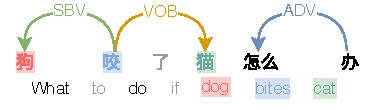
\includegraphics[scale=1.1]{figure/fig5-1-1.pdf}}

    \subfigure[被动语态(复述关系)]{\label{fig5-1-2}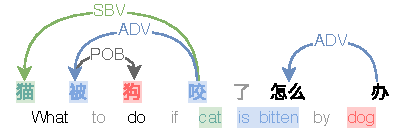
\includegraphics[scale=1.1]{figure/fig5-1-2.pdf}}

    \subfigure[被动语态(非复述关系)]{\label{fig5-1-3}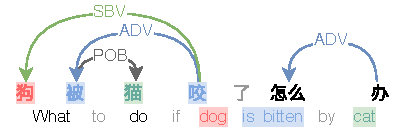
\includegraphics[scale=1.1]{figure/fig5-1-3.pdf}}
    \caption{主被动语态依存关系图}
    %Same words are with same color between example and corresponding translation.
    %'SBV'' to Subject-Predicate relation, 'ADV' refers to the relationship between adverbial and head word and 'POB' referfs to the relationship between preposition and object.
    \label{fig5-1}
\end{figure}

\subsection{语境特征}

语境(语言使用的场景)对语言表达有着一定的影响。
在大多数的非正式语境下,语言的表达有着随意性、简散性等特点,人类易懂但却对模型的鲁棒性提出了极大的挑战。
CQM$_{robust}$包含如下几种日常语境下的特征:

\begin{enumerate}
    \item \textbf{错别字:}
    在非正式书面用语中,错别字是最常见的一种语言错误。
    多数情况下,拼写错误并不影响人们的正常理解与交流,如例E30,{\kai“文身”}是网络上表达{\kai“纹身”}的一种常见错别字。
    神经网络模型也应该有能力察觉句子中的错别字并理解其真实意图,才能提高搜索引擎与问答系统等应用的容错率,提高用户体验感。
    \item \textbf{简单/复杂冗余:}
    冗余指的是句子中权重较低,对整句话的所传达的信息贡献不大仅用以凸显语境的部分,包括礼貌用语、问候、感叹等一些前置或后置的表达。
    如例E31与E32中的绿色部分,均为不同程度的冗余表达。
    该类别考察了模型的抗干扰能力,模型应当摒弃冗余表达的语义信息、捕获关键交互线索,
    借以判别出两个问句为语义相同的复述关系。
\end{enumerate}


\section{CQM$_{robust}$数据构造方案}

CQM$_{robust}$是一个多元化、自然化的中文数据集,其构建过程分为四个步骤。
如图~\ref{fig5-2}~所示,本章首先对源问题进行预处理操作,以便于加入符合语言学的扰动构造新问题。
然后,本章会对新问题进行是否为“自然语言”的检查,确保新问题必须是真实可靠的自然语言问句。
最后,本章将源问题和被扰乱的新问题配对作为一条样本,并由专门的数据审核人员对这些样本进行人工标注。
本小节将详细介绍CQM$_{robust}$的具体构建细节。

\begin{figure}[h]
    \centering
      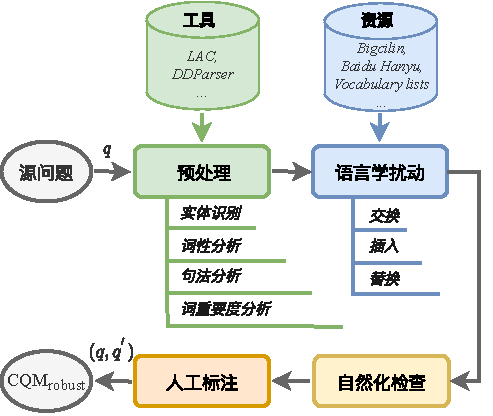
\includegraphics[scale=0.95]{figure/fig5-2.pdf}
    \caption{CQM$_{robust}$构造流程图}
    \label{fig5-2}
\end{figure}

\subsection{源问题预处理}

本节首先从百度搜索引擎的日志中收集了大量的源问题,所有的源问题都是用户提问的真实自然问句。
然后本章对源问题进行如下几个语言学预处理:

\begin{enumerate}
    \item \textbf{词性标注(Part-Of-Speech Tagging,简称POS Tagging):}
    借助百度中文词法分析工具(Lexical Analysis of Chinese,简称LAC)\footnote{https://github.com/baidu/lac}
    对源问题中的所有单词进行词性标注,便于体系化的对不同词性的词进行语言学扰动。
    \item \textbf{词重要性分析(Word Importance Analysis):}
    使用LAC工具标记出源问题中所有单词的权重(权重之和为1),单词的权重数值越大,则越能代表问句的语义走向。
    CQM$_{robust}$着重考察权重较高的词对源问题的影响。
    \item \textbf{命名实体识别(Named Entity Recognition,简称NER):}
    同样借助LAC工具标识出源问题中的实体,在小节~\ref{5.2.1 词法特征}~的命名实体子类别中详细介绍了如何利用这些实体设计测试样例。   
    \item \textbf{依存句法分析(Dependency Parsing):}
    借助百度依存句法分析工具(BaiDu Dependency Parser,简称DDParser)\footnote{https://github.com/baidu/DDParser}
    对源问句进行分析,
    从而设计相应的启发式规则构造如~\ref{5.2.2 句法特征}~小节所述的几种句法特征数据。
\end{enumerate}

\subsection{语言学扰动}

\begin{enumerate}
\item \textbf{词法特征:}
对于词法特征而言,
本章将源问题中的目标词替换为扰动词,或者将扰动词插入目标词前后。
所有的扰动词均通过如下几种方式收集:  
1) \textbf{Elasticsearch(简称ES)\footnote{https://github.com/elastic/elasticsearch}:}
从ES数据词典中检索与原词字面重叠的扰动词,如{\kai“空调”}和{\kai“空调扇”}。
2) \textbf{Faiss\footnote{https://github.com/facebookresearch/faiss}:}
从预先处理好的Faiss工具中查找与原词语义相近的扰动词,如{\kai“猕猴桃”}和{\kai“奇异果”}。
3) \textbf{Bigcilin\footnote{http://www.bigcilin.com/browser/}:}
从百度汉语词典中收集原词的同义词与反义词。
4) \textbf{XLM-RoBERTa\cite{conneau2019unsupervised}:}
将源问题中的目标词替换[MASK]特殊标记,
然后送入预训练语言模型XLM-RoBERTa中,
根据上下文预测出[MASK]位置的词作为扰动词。
5) \textbf{Vocabulary lists:}
本章预定义的一些特殊词汇表,如否定词表、时间词表。

\item \textbf{句法特征:}
对与句法特征而言,
本章首先从百度搜索日志中检索出与源问题编辑距离小于4的一些候选问题,
然后通过对比源问题与候选问题的依存结构,
将包含对称角色和非对称角色的问题对子保留,用于构造对应类别的测试样本。
同时,本章依据源问题和候选问题中的{\kai“被”}字特征以及主谓宾语法结构特征,
构造了一批主被动转换的样本。

\item \textbf{语境特征:}
本章借助中文错别字字典将源问题中的某一个字替换为常见的错别字。
对于冗余类别,本章插入一些疑问词、礼貌用语等在源问题中增加简单冗余表达,
并从百度高频问答日志中挑选一些长度差较大的复述问句作为复杂冗余样例。
\end{enumerate}


\subsection{自然化检查}

本章仅保留在近三个月的百度搜索日志中出现频率大于等于3次的扰动问句,以确保问句的质量和自然性,使得CQM$_{robust}$能有效地评估模型的实际应用能力。

\subsection{人工标注}

源问题和扰动问题组成的样例由百度内部数据团队进行人工审核。
首先,标注人员需要检查样本是否流畅、语法是否正确,以及标签(复述/非复述)是否合理。
低质量的样本将被丢弃,标签不合理样本的将被调整到其他测试类别或丢弃。
然后,这些样本将再由标注人员进行二轮审核,
每个样本由三位标注人员审核,两位或者两位以上的专家认同才算合格。
最终,从合格样本中随机选取10\%的样本由语言学专家进行审查,如果审查通过率小于95\%,
则数据团队需要对所有样本进行重新标注。

最终,CQM$_{robust}$包含10,121条高质量的自然问题对,表~\ref{table5-3}~和表~\ref{table5-2}~中分别展示了CQM$_{robust}$的统计信息与各个类别的详细信息。

% 表: train/dev/test description
\begin{table}
    \caption{CQM$_{robust}$数据统计}
    % \begin{spacing}{1.4}
    % \scriptsize
    \centering
    \newcommand{\tabincell}[2]{\begin{tabular}{@{}#1@{}}#2\end{tabular}}
    \setlength{\tabcolsep}{2mm}{
    \begin{tabular}{c|cc|ccc}
    \toprule[0.7pt]
    \multirow{2}{*}{\tabincell{c}{\textbf{类别}}} & \multicolumn{2}{c|}{\textbf{长度}} & \multicolumn{3}{c}{\textbf{数量}}  \\
      & \; 源问题\; & \;扰动问题 \; & \;复述 \; & \;非复述  & 全部  \\
    \midrule[0.7pt]
    \enspace{词法特征}\enspace  & 8.58 & 8.89  & 1,315 & 6,784  & 8,099               \\
    {句法特征}  & 9.86 & 9.89  & 678    & 532  & 1,210               \\
    {语境特征}   & 8.73    & 9.03    & 812  & 0 & 812                \\
    % {Speech Filler}     & 9.66    & 10.37   & 344  & 0   & 344                \\ 
    \midrule[0.7pt]
    \textbf{汇总}   & 8.74    & 8.90    & 2,805   & 7,316   & 1,0121              \\
    \bottomrule[0.7pt]
    \end{tabular}}
    \label{table5-3}
    % \end{spacing}
\end{table}

\section{实验及结果分析}

\subsection{数据集与评价方法}

本章在LCQMC数据集上对模型进行微调训练,并在CQM$_{robust}$上评估模型的性能。
LCQMC是由哈尔滨工业大学构造的一个大规模的中文问题复述语料库,数据集的详细介绍见~\ref{2.2 语料资源概述}~小节。

本章提倡除了采用传统的\textbf{微平均准确率(Micro-accuracy)}计算模型对CQM$_{robust}$中所有样本分类准确率的算术平均值,
还应当以样本类别为单位,采用\textbf{宏平均准确率(Macro-accuracy)}计算模型对32种不同数据分类准确率的算术平均值。
往往欺骗性越强的样本类别,其构造难度越大,即在CQM$_{robust}$中的样本数量越少。
采用宏平均准确率可以忽略多类别数据集中由样本数量差造成的性能偏差。


\subsection{基线模型与超参设置}

本章选用了6种采用不同预训练策略或参数规模的语言模型进行实验,包括:
$base$参数规模的BERT\cite{devlin2018bert}、ERNIE\cite{sun2019ernie}、RoBERTa\cite{liu2019roberta}和MacBERT\cite{cui2020revisiting}模型,
以及$large$参数规模的RoBERTa和MacBERT模型。
% BERT$_{base}$\cite{devlin2018bert}、ERNIE$_{base}$\cite{sun2019ernie}、
% RoBERTa$_{base}$RoBERTa$_{large}$\cite{liu2019roberta}
% MacBERT$_{base}$和MacBERT$_{large}$\cite{cui2020revisiting}。
本章所有模型输入问题对的最大长度限制为65,训练阶段batch\_size均设置为64。
对于${base}$规模的模型,优化器的学习率设置为5e-6,训练3轮。
对于${large}$规模的模型,优化器的学习率设置为2e-5,训练2轮。
为防止实验误差,本章的所有实验均进行3次取平均结果。


\subsection{CQM$_{robust}$评估结果分析}


\textbf{挑战性更高:}
表~\ref{table5-4}~展示了基线模型在LCQMC$_{test}$和CQM$_{robust}$上的评估结果。
其中,下标$b$表示模型为$base$规模,下标$l$表示模型为$large$规模,加粗和下划线分别标识出在测试集上表现最佳和第二的模型性能。
显而易见,所有模型在LCQMC$_{test}$上的准确率均高于87\%,
但是在CQM$_{robust}$上的性能却明显下降,$\triangle$表示两者性能差,最大性能差可达20.5\%。
由此说明,CQM$_{robust}$更具有挑战性,能有效地反应问题复述识别模型的真实能力。

% 表: 实验总体性能
\begin{table}
    \caption{LCQMC$_{test}$和CQM$_{robust}$实验性能对比}
    % \begin{spacing}{1.4}
    \centering
    % \scriptsize
    \newcommand{\tabincell}[2]{\begin{tabular}{@{}#1@{}}#2\end{tabular}}
    \begin{tabular}{c|c|c|c}
    \toprule[0.7pt]
    \textbf{模型} & \enspace \textbf{LCQMC$_{test}$}\enspace  & \enspace \textbf{CQM$_{robust}$} \enspace & \enspace \textbf{$\triangle$} \\
    \midrule[0.7pt]
    BERT\textsubscript{b} &87.1±0.1 &66.6±0.6 & \enspace -20.5\\
    ERNIE\textsubscript{b} & 87.3±0.1& 69.8±0.3 &\enspace -17.5 \\
    RoBERTa\textsubscript{b} & 87.2±0.4&69.5±0.1 &\enspace -17.7\\
    \enspace MacBERT\textsubscript{b}\enspace  &87.4±0.3 &70.3±0.6 &\enspace -17.1\\
    \hline
    RoBERTa\textsubscript{l} & \textbf{87.7±0.1}&\textbf{73.8±0.3} &\enspace -13.9\\
    MacBERT\textsubscript{l} &\underline{87.6±0.1} &\underline{73.8±0.5} &\enspace -13.8\\
    \bottomrule[0.7pt]
    \end{tabular}
    \label{table5-4}
    % \end{spacing}
\end{table}
    

\textbf{辨别能力更强:}
值得注意的是,所有的基线模型在LCQMC$_{test}$上均有着相近的性能结果,约为87\%。
但在CQM$_{robust}$上,$base$模型的性能从66.6\%到70.3\%不等,$large$模型的最高性能更是达到了73.8\%。
可以看出,CQM$_{robust}$能更加明显展现出模型的性能差异,对模型具有更高的区分度。

\textbf{评估角度更多样:}
CQM$_{robust}$是一个细粒度的评估基准,
其包含3大类特征类别、13个测试子类,共计32种数据测试项,
可以根据不同的语言现象对模型进行详细的评估。
本章采用多个基线模型在CQM$_{robust}$上的进行实验,实验结果如表~\ref{table5-2}~和表~\ref{table5-5}~所示。
通过对比不同模型在各个测试项上的表现差异,本节得出如下结论:

\begin{table}
    \caption{CQM$_{robust}$详细评估结果}
    % \begin{spacing}{1.1}
    % \scriptsize
    \centering
    \newcommand{\tabincell}[2]{\begin{tabular}{@{}#1@{}}#2\end{tabular}}
    \resizebox{155mm}{38mm}
    {
    \begin{tabular}{cc|cccccc|c|c|c|c}
    \toprule[0.7pt]
    \multicolumn{2}{c|}{\multirow{2}*{\textbf{\tabincell{c}{模型}}} }
     & \multicolumn{7}{c|}{\textbf{词法}} & \multirow{2}*{\textbf{句法}} & \multirow{2}*{\textbf{语境}} & \multirow{2}*{\textbf{CQM$_{robust}$}} \\
    \multicolumn{2}{c|}{ }& 基础词汇 & 命名实体 & 同义词 & 反义词 & 否定 & 时态 & \textbf{词法} &  &  & \\
     \midrule[0.7pt]
    \multirow{2}*{\tabincell{c}{BERT\textsubscript{b}}} & micro & 62.1±1.1 & 92.3±0.5 & 69.5±0.4 & 50.6±3.4 &
    64.4±5.9 & 35.1±3.3 & 67.2±0.7 & 59.1±0.4 &
    72.6±1.6 & 66.6±0.6  \\
    & macro & 51.9±1.5 & 91.2±0.7 & 76.4±0.6 & 50.6±3.4 &
    57.6±4.4 & 35.5±3.3 & 61.4±1.2 & 59.1±0.7 &
    71.1±1.1 & 62.0±0.9  \\\hline
    
    \multirow{2}*{\tabincell{c}{ERNIE\textsubscript{b}}} & micro & 64.6±0.5 & \underline{92.8±0.4} & 73.2±0.9 & 69.6±2.9 &
    77.8±1.1 & 48.0±1.9 & 71.0±0.3 & 60.0±1.2 &
    72.4±0.3 & 69.8±0.3  \\
    & macro & 52.4±0.7 & \underline{92.3±0.6} & 79.5±0.7 & 69.6±2.9 &
    69.1±1.2 & 48.5±1.9 & 65.5±0.5 & 56.5±1.0 &
    73.2±0.8 & 65.1±0.3  \\\hline
    
    \multirow{2}*{\tabincell{c}{RoBERTa\textsubscript{b}}} & micro & 64.2±0.1 & 90.6±1.8 & 74.2±1.4  &65.0±1.5 & 76.3±1.7 & 43.7±0.2 &
    70.1±0.1 & 63.1±0.6 & 73.3±0.1 & 69.5±0.1  \\
    & macro & 53.3±0.2 & 89.4±2.5 & 80.3±1.1 & 65.0±1.5 & 68.8±1.3 & 44.0±0.2 &
    65.0±0.1 & 60.9±0.6 & 75.6±0.5 & 65.5±0.1 \\\hline
    
    \multirow{2}*{\tabincell{c}{MacBERT\textsubscript{b}}} & micro & 64.8±1.1 & 92.0±0.7 & 73.3±1.1  & 73.1±4.3 & \underline{80.7±0.5} & 47.6±1.3 &
    71.2±0.7 & 62.1±1.0 & \underline{73.4±1.5} & 70.3±0.6  \\
    & macro & 54.2±0.9 & 90.7±0.6 & 79.7±0.5 & 73.1±4.6 & 70.7±0.1 & 47.7±0.2 &
    66.3±0.2 & 55.5±0.7 & 75.2±1.1 & 65.8±0.1  \\\hline
    
    \multirow{2}*{\tabincell{c}{RoBERTa\textsubscript{l}}} & micro & \textbf{67.2±0.9} &
    92.5±0.3 & \underline{76.0±2.1} & \textbf{91.7±2.3} & 80.2±0.8 & \textbf{58.6±2.8} &
    \underline{74.1±0.3} &
    \textbf{72.6±1.4} &
    73.2±1.9 &
    \textbf{73.8±0.3}  \\
    & macro & \textbf{57.7±0.6} &
    91.6±0.3 & \underline{81.7±1.6} & \textbf{91.7±2.3} & \underline{72.3±0.6} & \textbf{59.0±2.7} &
    \underline{70.2±0.3} &
    \textbf{63.4±1.2} &
    \underline{76.0±2.0} & \underline{69.8±0.2}  \\\hline
    
    \multirow{2}*{\tabincell{c}{MacBERT\textsubscript{l}}} & micro & \underline{65.6±0.8} &
    \textbf{93.2±0.6} & \textbf{83.2±1.6} & \underline{90.7±2.3} & \textbf{84.3±1.3} & \underline{55.5±4.0} &
    \textbf{74.4±0.4} &
    \underline{70.2±3.7} &
    \textbf{73.7±1.1} &
    \underline{73.8±0.5}  \\
    & macro & \underline{54.7±0.9} &
    \textbf{92.6±0.9} & \textbf{87.1±1.2} & \underline{90.7±2.3} & \textbf{78.1±0.9} & \underline{56.1±4.0} &
    \textbf{70.7±0.5} &
    \underline{61.6±2.4} &
    \textbf{77.1±0.6} & \textbf{70.2±0.5}  \\
    
    \bottomrule[0.7pt]
    \end{tabular}
    }
    \label{table5-5}
    % \end{spacing}
\end{table}
    
    % \setlength{\tabcolsep}{1.5mm}{

\begin{enumerate}
    \item 如表~\ref{table5-5}~所示,绝大部分测试类别的最优及次优性能集中在表格下半部分,即$large$模型的表现总体优于$base$模型。
    因为$large$模型的参数规模更大且训练语料更丰富,所以它们比$base$模型具有更强的能力。
    \item 在实体识别子类中,ERNIE$_{base}$的表现优于其他${base}$模型和RoBERTa$_{large}$模型,
    这是由于ERNIE在预训练的过程中加入了实体掩码策略,这有利于强化模型对实体词汇的识别能力。
    \item MacBERT$_{large}$模型在同义词子类表现最佳,这得益于它在预训练中采用了相近词掩码策略
    强化了模型对同义词的辨别能力。
    \item 所有模型在时态子类特征上的表现均较差,这说明模型对中文时间词所导致的语义差异缺乏敏感性。
    \item 在句法特征中,模型对于对称角色的感知能力要远远高于非对称角色。
    本文认为模型并未真正理解词语在句子中所扮演的角色,而仅仅是倾向于将字面重叠度高的两个问句判别为复述关系。
    \item ${base}$模型在错别字类别上表现要优于${large}$模型,
    这是由于${large}$模型的训练更加充分,间接导致了其对与错别字的感知更加敏感。
\end{enumerate}

\subsection{对抗训练分析}

CQM$_{robust}$是一个符合语言特征的自然问句数据集,有利于客观评估模型的鲁棒性。
为了证明这一点,本章使用两种对抗攻击产出的样本进行对抗训练实验,包括:
基于Wordnet的同义词替换攻击PWWS\cite{ren2019generating};基于Word2vec的同义词替换攻击TEXTFOOLER\cite{jin2020bert}。
并且,本章将这些强化后的模型在多种数据上进行交叉评估。
如表~\ref{table5-6}~所示,除了CQM$_{robust}$以外,
这些评估数据还包括:从对抗性样本中人工选取了200条自然样本子集PWWS\textsubscript{nat}和TEXTFOOLER\textsubscript{nat} ;
从CHECKLIST中文翻译数据中人工选取了400条问题对子集CHECKLIST\textsubscript{nat}。

% 表: 对抗数据量统计
\begin{table}
    % \begin{spacing}{1.4}
    \caption{对抗数据统计}
    \centering
    \footnotesize
    \newcommand{\tabincell}[2]{\begin{tabular}{@{}#1@{}}#2\end{tabular}}
    \setlength{\tabcolsep}{1.2mm}{
    \begin{tabular}{l|cc|cc|c}
    \toprule
    &PWWS & \enspace PWWS\textsubscript{nat} \enspace &\enspace TEXTFOOLER \enspace &\enspace TEXTFOOLER\textsubscript{nat} \enspace &\enspace CHECKLIST\textsubscript{nat}\\
    \midrule[0.7pt]
    训练数据\quad\ & \enspace 159,503\enspace&-& 64,086&-& \enspace -\\
    测试数据 &400&200&400&200&\enspace400 \\
    \bottomrule[0.7pt]
    \end{tabular}
    }
    \label{table5-6}
    % \end{spacing}
\end{table}
    

本章使用RoBERTa$_{large}$基线模型在LCQMC数据上进行对抗训练,实验结果如表~\ref{table5-7}~所示。
显而易见,经过对抗训练强化后的模型在PWWS和TEXTFOOLER测试数据上均有大幅提升。
但是,在经过人工筛选后的PWWS\textsubscript{nat}、TEXTFOOLER\textsubscript{nat}上,
并没有获得期望的性能提升。
同样,在CHECKLIST\textsubscript{nat}以及CQM$_{robust}$上也无明显提升,甚至略有下降。

% 表: 对抗训练性能结果
\begin{table*}[!h]
    \begin{spacing}{1.4}
    \scriptsize
    \caption{对抗训练性能对比} 
    \centering
    \newcommand{\tabincell}[2]{\begin{tabular}{@{}#1@{}}#2\end{tabular}}
    \begin{tabular}{lc|cc|cc|c|cc}
    \toprule[0.7pt]
    %  \multirow{2}*{\textbf{Model}} &
     \multirow{2}*{\textbf{训练数据}} & \multirow{2}*{\textbf{LCQMC}} & \multicolumn{4}{c|}{\textbf{对抗数据}} & \multirow{2}*{\textbf{CHECKLIST\textsubscript{nat}}} & \multicolumn{2}{c}{\textbf{CQM\textsubscript{robust}}} \\
     & & PWWS & PWWS\textsubscript{nat}& TEXTFOOLER & TEXTFOOLER\textsubscript{nat}& & Micro & Macro\\
    \midrule[0.7pt]
    
     LCQMC & \underline{87.7} & 58.1 & 81.5& 57.1 & 87.8& \underline{76.9} & \underline{73.8} & 69.8 \\
    
    %  LCQMC+PAWS &87.4\textcolor{textred}{\textsubscript{-0.3}} & 61.5\textcolor{textgreen}{\textsubscript{+3.4}} & 81.8\textcolor{textgreen}{\textsubscript{+0.3}}&58.3\textcolor{textgreen}{\textsubscript{+1.2}} & \underline{88.0}\textcolor{textgreen}{\textsubscript{+0.2}}& 76.4\textcolor{textred}{\textsubscript{-0.5}} & 73.2
    % \textcolor{textred}{\textsubscript{-0.6}} & \textbf{70.6}\textcolor{textgreen}{\textsubscript{+0.8}} \\
    
     LCQMC+PWWS & \underline{87.7}\textcolor{textgreen}{\textsubscript{+0.0}} & \textbf{97.6}\textcolor{textgreen}{\textsubscript{+39.5}} & 81.8\textcolor{textgreen}{\textsubscript{+0.3}}& \underline{73.1}\textcolor{textgreen}{\textsubscript{+16.0}} & 87.6\textcolor{textred}{\textsubscript{-0.2}}& 76.0\textcolor{textred}{\textsubscript{-0.9}} & \textbf{75.2}
    \textcolor{textgreen}{\textsubscript{+1.4}} & \underline{70.4}\textcolor{textgreen}{\textsubscript{+0.6}} \\
    
     LCQMC+FOOLER & 87.5\textcolor{textred}{\textsubscript{-0.2}} & \underline{78.5}\textcolor{textgreen}{\textsubscript{+20.4}} & \textbf{83.8}\textcolor{textgreen}{\textsubscript{+2.3}}& \textbf{80.8}\textcolor{textgreen}{\textsubscript{+23.7}} & 82.0\textcolor{textred}{\textsubscript{-5.8}}&\textbf{79.2}\textcolor{textgreen}{\textsubscript{+2.3}} & 71.4
    \textcolor{textred}{\textsubscript{-2.4}} & 68.8\textcolor{textred}{\textsubscript{-1.0}} \\
    
    % \midrule[0.4pt]
    
    % Ensemble & LCQMC &\textbf{88.0}\textcolor{textgreen}{$_{+0.3}$}&\underline{83.3}\textcolor{textgreen}{$_{+1.8}$} &60.3\textcolor{textgreen}{$_{+2.2}$}& \textbf{89.5}\textcolor{textgreen}{$_{+1.7}$}&54.3\textcolor{textred}{$_{-2.8}$}& 73.4\textcolor{textred}{$_{-3.5}$} & 72.0\textcolor{textred}{$_{-1.8}$} & 67.4\textcolor{textred}{$_{-2.4}$} \\
    
    
    \bottomrule[0.7pt]
    \end{tabular}
    \label{table5-7}
    \end{spacing}
\end{table*}

由此可见,常见的对抗性样本在自然评估数据集上效果并不明显,仅在与之分布一致的样本上有所效果。
作为一个符合语言学特征的自然化中文语料库,CQM$_{robust}$有利于模型的鲁棒性评估,
能够间接提高模型在现实世界中的应用能力。

\section{本章小结}

本章构造了一个多样化、自然化的中文数据集CQM$_{robust}$,用于评估问题识别复述模型的综合能力及鲁棒性。
CQM$_{robust}$包含3种语言特征、13个测试子类,共计32种蕴含不同语言学特征的测试项,其样本均来自于百度搜索日志中的用户真实提问。
实验证明,CQM$_{robust}$中的样本难度更大、更加具有挑战性,
且其细粒度的评估体系有助于诊断模型的优势与缺陷,使研究人员能够以更加多样化的方式分析模型。

\chapter{总结与展望}

\section{工作总结}

问答匹配是文本匹配领域的主要研究方向之一,
根据数据源的不同通常将其划分为答案选择和问题复述识别两个子任务。
答案选择任务关注“问题与答案”间的语义关系,根据目标问题从大规模候选答案中挖掘相关的正解,用以优化智能问答场景下召回相关答案的质量。
问题复述识别关注“问题与问题”间的语义关系,根据目标问题从候选问题集合中寻找同义问题(已知答案),并将其答案作为目标问题的正解反馈给用户。
目前预训练语言模型等深度模型在问答匹配领域已经取得一定进展,
然而在该任务中仍存在一些有待解决的问题,包括模型对精细语义不够敏感以及缺乏鲁棒性。
本文针对上述问题,提出一种基于精细语义感知和鲁棒性诊断的问答匹配方法,具体地工作总结如下:

\textbf{\songti (1)基于多粒度交互推理的答案选择方法研究}

本文发现不同粒度的语义成分,皆有助于预测问题与答案的局部语义关联性,形成多粒度的关联线索。
所以,本文提出一种多粒度交互式推理网络MIIN,其基于BERT编码特征二次进行多粒度卷积编码,
并且将多粒度交互信息与原始分类特征融合,保留问题与答案交互过程中的精细语义线索。
此外,长文本候选答案中不同子句与问题的关联性具有明显差异,
本文设计一种子句损失优化策略,侧重提升关键语句在答案选择过程中的作用。

\textbf{\songti (2)面向问题复述识别的定向数据增强方法}

本文提出一种定向数据增强策略DDA,用于提高问题复述识别模型对问题精细语义的感知能力。
其通过在生成模型UNILM的输入中添加定向诱导标签,生成期望的复述句或非复述句。
相较于传统的数据增强方案,DDA能有效降低文本的语法错误率,并且产出的样本质量更高、难度更大。
DDA为预训练语言模型的微调扩充了大量蕴含精细语义关系的问题对子样本,有效提高了模型对细微语义感知。

\textbf{\songti (3)面向问题复述识别的模型综合能力鲁棒性研究}

鲁棒性是反应模型能力的一项重要评价指标,能够检验模型在面对微小变化时的稳定性,也是模型泛化能力的体现。
本文构造了一个面向中文问题复述识别模型的评估基准CQM$_{robust}$,其包含3大类语言特征、13个测试子类,共计32个测试项。
CQM$_{robust}$中的所有问句均来自于百度搜索日志中的真实问题,能够更加客观反映模型的实际应用能力。
实验结果证明,CQM$_{robust}$更具有挑战性,且能够对按照语言学现象对模型的鲁棒能力进行详细评估。

\section{工作展望}

本文对问答匹配技术展开研究,提出一种基于精细语义感知和鲁棒性诊断的问答匹配方法,
在一定程度上解决了当前问答匹配领域存在的难点问题。
然而,其中仍存在可以改进的地方:

\textbf{\songti (1)优化特征融合的方式}

本文所提出的多粒度交互式推理方法中,直接采用拼接的方式将多种粒度的交互特征以及原始的分类特征进行融合。
然而,不同粒度特征信息的权重不同。
因此,在未来的工作中,可以考虑使用可训练的参数将不同粒度的信息进行加权融合,让模型在训练过程中对参数进行自我调节。

\textbf{\songti (2)生成更加多样化的问句}

本文所提出的定向数据增强策略,通过给定诱导标签能够控制生成模型问句的类型(复述或非复述)。
然而,诱导标签中包含的信息量过于单一,生成的问句中仍保留有绝大部分的原始问句信息,从而导致生成问句的语义大多都倾向于与原始问句语义近似。
因此,在后续工作中,应当考虑在生成过程中引入其他附加信息或计算操作,用以扩大生成问句与原始问句的差异,使生成的问句更加多样化。

\textbf{\songti (3)扩增语料的语种类型}

本文所构造的CQM$_{robust}$能够系统化的评估问题复述识别模型的鲁棒能力,并且其所有样本均为自然问句。
然而,CQM$_{robust}$中仅包含符合中文语言特征的样本,只能对中文问题复述识别模型作出详细诊断。
因此,在后续工作中,可以尝试对英文等语言现象进行分析,在数据集中加入其他语种的样本,
使得CQM$_{robust}$不仅能评估多种语言的问题复述识别模型,甚至能评估模型的跨语言理解能力。



% % 参考文献,4或者小4楷体
\phantomsection
\addcontentsline{toc}{chapter}{参考文献}
\begin{kai}
    \bibliography{reference}
\end{kai}

% % 附录,4或者小4楷体
% \appendix

% 附页标题样式
\backmatter
% 附页
\chapter{攻读学位期间的成果}

\vspace{8pt}
%% 盲审版本匿名化成果
% \begin{enumerate}[itemsep=0.7em, leftmargin=2em, itemindent=0em,labelwidth=2em]
% 	\item[1.] 中文信息学报. 已录用. 第一作者
% 	\item[2.] 中文信息学报. 已录用. 第一作者
% 	\item[3.] Proceedings of the 2021 Conference of the International Conference on Asian Language Processing (IALP), 2021 .第一作者
% 	\item[4.] Proceedings of the 2022 Conference of the North American Chapter of the Association for Computational Linguistics (NAACL), 2022. 已投出. 第一作者
% 	\item[5.] 中文信息学报. 已录用. 第三作者
% 	\item[6.] Proceedings of the 44th European Conference on Information Retrieval (ECIR), 2022. 第三作者
% 	\item[7.] 中文信息学报, 2021. 第三作者
% 	\item[8.] Proceedings of the 2022 Conference of the International Joint Conference on Neural Networks (IJCNN), 2022. 已投出. 第三作者
% \end{enumerate}

% 盲审版本匿名化成果
% \begin{enumerate}[itemsep=0.7em, leftmargin=2em, itemindent=0em,labelwidth=2em]
% 	\item[1.] Proceedings of the 44th European Conference on Information Retrieval (ECIR), 2022. 第一作者 (\textbf{CCF C})
% 	\item[2.] Proceedings of the 44th European Conference on Information Retrieval (ECIR), 2023. 第一作者 (\textbf{CCF C})
% 	\item[3.] Proceedings of the 60th Annual Meeting of the Association for Computational Linguistics (ACL), 2023. 已投出 第一作者 (\textbf{CCF A})
% 	\item[4.] 中文信息学报. 已录用 第一作者 (\textbf{核刊}) 
% 	\item[5.] Proceedings of the 2021 Conference of the International Conference on Asian Language Processing (IALP), 2021 .第二作者 \textbf{EI} 
% 	\item[6.] 中文信息学报. 已录用. 第二作者 (\textbf{核刊}) 
% 	\item[7.] Proceedings of the 44th European Conference on Information Retrieval (ECIR), 2023. 第三作者 (\textbf{CCF C})
% 	\item[8.] 山西大学学报. 已录用. 第四作者 (\textbf{核刊}) 
% \end{enumerate}

%% 非盲审版本成果
% \begin{enumerate}[itemsep=0.7em, leftmargin=2em, itemindent=0em,labelwidth=2em]
% 	\item[1.] \textbf{朱鸿雨},洪宇,苏玉兰,唐竑轩,尉桢楷,张民. 基于多粒度交互推理的答案选择方法研究. 中文信息学报. 已录用.(\textbf{核刊})
% 	\item[2.] \textbf{朱鸿雨},金志凌,苏玉兰,张民,洪宇. 面向问题复述识别的定向数据增强方法. 中文信息学报. 已录用.(\textbf{核刊})
% 	\item[3.] \textbf{Hongyu Zhu}, Yan Chen, Jing Yan, Jing Liu, Yu Hong, Ying Chen. CQM$_{robust}$: A Chinese Dataset of Linguistically Perturbed Natural Questions for Evaluating the Robustness of Question Matching Models. EMNLP 2022.待投出. (\textbf{CCF B})
% 	\item[4.] \textbf{Hongyu Zhu}, Zhiling Jin, Yan Bai, Yu Hong, Min Zhang. Multi-granularity Interaction Fusion for Neural Answer Source Selection[C]//Proceedings of the 2021 Conference of the International Conference on Asian Language Processing (IALP). IEEE, 2021: 13-18. (\textbf{EI})
% 	\item[5.] 苏玉兰,洪宇,\textbf{朱鸿雨},武恺莉,张民. 基于大规模问答数据的噪声感知问题生成. 中文信息学报. 已录用.(\textbf{核刊})
% 	\item[6.] Zhiling Jin, Yu Hong, \textbf{Hongyu Zhu}, Jianmin Yao, Min Zhang. Bi-granularity Adversarial Training for Non-Factoid Answer Retrieval[C]//Proceedings of the European Conference on Information Retrieval. Springer, Cham, 2022: 322-335. (\textbf{CCF C})
% 	\item[7.] 武恺莉,朱朦朦,\textbf{朱鸿雨},张熠天,洪宇. 结合问题类型及惩罚机制的问题生成[J]. 中文信息学报, 2021, 35(4): 110-119.(\textbf{核刊})
% 	\item[8.] Yulan Su, Yu Hong, \textbf{Hongyu Zhu}, Minhan Xu, Yifan Fan. Binary-perspetive Asymmetrical Twin Gain: a Novel Evaluation Method for Question Generation. IJCNN 2022. 已录用. (\textbf{CCF C})
% \end{enumerate}

% 非盲审版本成果
\begin{enumerate}[itemsep=0.7em, leftmargin=2em, itemindent=0em,labelwidth=2em]
	\item[1.] \textbf{Zhiling Jin}, Yu Hong, Hongyu Zhu, Jianmin Yao, Min Zhang. Bi-granularity Adversarial Training for Non-factoid Answer Retrieval[C]//Advances in Information Retrieval: 44th European Conference on IR Research, ECIR 2022, Stavanger, Norway, April 10–14, 2022, Proceedings, Part I. Cham: Springer International Publishing, 2022: 322-335. (\textbf{CCF C})
	\item[2.] \textbf{Zhiling Jin}, Yu Hong, Rui Peng Jianmin Yao, Guodong Zhou. Intention-aware Neural Networks for Question Paraphrase Identification. ECIR 2023 已录用. (\textbf{CCF C})
	\item[3.] \textbf{金志凌},朱鸿雨,苏玉兰,唐竑轩,洪宇,张民. 基于多粒度交互推理的答案选择方法研究. 中文信息学报. 已录用.(\textbf{核刊})
	\item[4.] \textbf{Zhiling Jin}, Yu Hong, Zhifeng Li, Jianmin Yao, Guodong Zhou. GBT: Generation Boosting Training for Sentence Semantic Matching. ACL 2023 已投出. (\textbf{CCF A})
	\item[5.] Hongyu Zhu, \textbf{Zhiling Jin}, Yan Bai, Yu Hong, Min Zhang. Multi-granularity Interaction Fusion for Neural Answer Source Selection[C]//Proceedings of the 2021 Conference of the International Conference on Asian Language Processing (IALP). IEEE, 2021: 13-18. (\textbf{EI})
	\item[6.] 朱鸿雨,\textbf{金志凌},苏玉兰,张民,洪宇. 面向问题复述识别的定向数据增强方法. 中文信息学报. 已录用.(\textbf{核刊})
	\item[7.] Rui Peng, Yu Hong, \textbf{Zhiling Jin}, Jianmin Yao and Guodong Zhou. Feature Differentiation and Fusion for Semantic Text Matching. ECIR 2023 已录用. (\textbf{CCF C})
	\item[8.] 李志峰,邹博伟,李烨秋,\textbf{金志凌},洪宇. 基于多知识源融合的级联式常识问答方法. 山西大学学报. 已录用. (\textbf{核刊})
\end{enumerate}
\chapter{致谢}

\vspace{8pt}
三年的研究生学业生涯即将结束,
由衷的感谢给予过我帮助的老师、同学和家人。
首先,感谢张民导师对我学业上的谆谆教导和生活上的悉心帮助。
张老师渊博的专业知识、严谨的治学态度,是我以后学习的榜样。
同时,还要感谢洪宇老师。
洪老师是我科研生涯的引路人,在学术研究上始终给予我悉心的指导,
并且鼓励和支持我们参加国内外学术交流活动,开阔了我们的视野。
在日常生活中,洪老师也时刻关注着我的心里和身体健康,帮助我们缓解学业压力,使实验室气氛积极融洽。

感谢周国栋、朱巧明、陈文亮、李培峰、李寿山、孔芳、姚建民、钱龙华、王红玲、段湘煜、李军辉、贡正仙、李正华、朱晓旭、邹博伟、周夏冰、王中卿等苏州大学自然语言处理实验的所有老师,
感谢他们为苏州大学自然语言处理实验室的同学们提供的优良实验氛围与计算资源。

其次,感谢实验室的所有同学们,
感谢李伟康、陈鑫、唐竑轩、白岩、黄荣涛、尉桢楷师兄以及武凯莉、朱朦朦、孙雨、陈佳丽师姐为我的科研提供的帮助和指导;
感谢同届的苏玉兰、王捷、钱锦、徐旻涵、李晓、潘雨晨、李烨秋同学,在三年共处时光里给予我的帮助和关心;
感谢师弟金志凌、李志峰、董梦星、刘皓、刘东、窦祖俊和师妹李中秋,感谢大家一起营造了实验室良好的氛围。

感谢我的父母和家人,你们始终默默地付出和奉献,没有您们对我的关心、支持和爱护,我无法顺利完成我的研究生学业。

最后,还要感谢参加论文评审和答辩的各位老师,感谢您们的批评与指导。

\vspace{10pt}
\begin{flushright}
    朱鸿雨

    2022年4月10日
\end{flushright}



% 
\includepdf[page=-]{pdf-pages/空白页.pdf}
% \includepdf[page=-]{pdf-pages/委员会决议.pdf}

\end{document}
